\documentclass[
    a4paper,        % Papierformat
    11pt,           % Schriftgröße
    ngerman,        % Sprache für Trennung und Bezeichnungen
    parskip=half,   % Halbe Zeile Abstand zwischen Absätzen (statt Einrücken)
    listof=totoc,   % Abbildungs-/Tabellenverzeichnis im Inhaltsverzeichnis
    bibliography=totoc % Literaturverzeichnis im Inhaltsverzeichnis
]{scrartcl}

% --- Grundlegende Pakete ---
\usepackage[utf8]{inputenc} % Kodierung (bei modernen Editoren oft Standard)
\usepackage[T1]{fontenc}    % Wichtig für Umlaute und Trennung
\usepackage{lmodern}        % Schöneres Schriftbild (Vektorschrift)
\usepackage{babel}          % Deutsche Bezeichnungen (Inhaltsverzeichnis etc.)

% --- Mathe und Technik ---
\usepackage{amsmath, amssymb, amsthm, nicefrac} % Mathematische Formeln
\usepackage{siunitx}        % WICHTIG für Einheiten: \SI{5}{\meter}
\sisetup{locale = DE}       % Komma statt Punkt als Dezimaltrenner

% --- Grafik und Tabellen ---
\usepackage{graphicx}       % Einbinden von Bildern
\usepackage{booktabs}       % Schönere Tabellenlinien (\toprule, \midrule, \bottomrule)
\usepackage{float}          % Um Bilder an exakten Stellen zu platzieren [H]

% --- Design und Layout ---
\usepackage[left=2.5cm, right=2.5cm, top=2.5cm, bottom=2.5cm]{geometry} % Ränder
\usepackage[headsepline]{scrlayer-scrpage} % Kopf- und Fußzeilen
\pagestyle{scrheadings}
\clearpairofpagestyles
\ihead{Erkennung von QR-Codes} % Kopfzeile links
\ohead{\today}              % Kopfzeile rechts
\cfoot{\pagemark}           % Seitenzahl unten mitte
\counterwithin{figure}{section} % Nummerierung der Abbildungen.

% Erzwingt, dass jede Section auf einer neuen Seite beginnt
\let\oldsection\section
\renewcommand\section{\clearpage\oldsection}

% --- Verlinkungen (sollte meist als letztes geladen werden) ---
\usepackage[hidelinks]{hyperref} % Klickbare Links im PDF, keine roten Rahmen

\usepackage{listings}
\usepackage{xcolor}
\graphicspath{{Images/}}

% Einfache Konfiguration für Python-Optik
\lstset{
    language=Python,
    basicstyle=\ttfamily\small,
    keywordstyle=\color{blue},
    commentstyle=\color{green!50!black},
    stringstyle=\color{orange},
    numbers=left,
    numberstyle=\tiny,
    frame=single,
    breaklines=true,
    captionpos=b
}
\begin{document}

% ==========================================
% DECKBLATT
% ==========================================
\begin{titlepage}
    \centering
    % Platzhalter für ein Logo (auskommentieren, wenn Bild vorhanden)
    % \includegraphics[width=0.4\textwidth]{logo.png} 
    \vspace{2cm}
    
    {\scshape\LARGE Hochschule Karlsruhe \par}
    \vspace{1cm}
    {\scshape\Large Fakultät für Maschinenbau \& Mechatronik \par}
    {\scshape\Large Studiengang Robotik und KI in der Produktion \par}
    \vspace{1.5cm}
    
    {\huge\bfseries Projektbericht zum Fach Künstliche Intelligenz \par}
    \vspace{0.5cm}
    {\Large Erkennung von QR-Codes \par}
    
    \vspace{2cm}
    
    % Autoren in einer Tabelle nebeneinander
    \vspace{2cm}
    \begin{center}
        \begin{tabular}{l p{2cm} l}
            Marlon Leitschuh    & & Nico Sander \\
            Matrikelnr: 103626  & & Matrikelnr: 74808 \\
            lema1046@h-ka.de    & & sani1019@h-ka.de.de \\
        \end{tabular}
    \end{center}

    \vfil

    \textbf{Betreuung:} \\
    Prof. Dr. -Ing. habil. Catherina Burghart

    \vspace{0.8cm}
    
    \textbf{Datum:} \\
    \today
    
\end{titlepage}

% ==========================================
% VERZEICHNISSE
% ==========================================
\tableofcontents            % Inhaltsverzeichnis
\newpage
\listoffigures              % Abbildungsverzeichnis
\newpage

% ==========================================
% INHALT
% ==========================================

\section{Einleitung} \label{sec:einleitung}

Zur Steuerung des Waschprozesses und der gewählten Zusatzoptionen gibt die Waschanlage einen Beleg mit QR-Code aus, welcher hinter der Windschutzscheibe zu positionieren ist. Eine zentrale Anforderung an das System ist die kontinuierliche Erfassung dieses Codes durch eine Kamera, sowohl vor als auch während des Waschvorgangs. Die Lesbarkeit muss hierbei auch unter erschwerten Bedingungen, etwa durch Verschmutzungen, Nässe oder Schaumbildung auf der Scheibe, gewährleistet sein. Des Weiteren ist zu berücksichtigen, dass sich im Sichtfeld potenziell diverse Störobjekte oder weitere Schriftstücke (mit oder ohne QR-Codes) befinden können.
%
\subsection{Aufgabenstellung} \label{subsec:aufgabenstellung}

\subsubsection{Klassifikation} \label{subsubsec:aufgabenstellung_klassifikation}

Ein Kernziel ist die Entwicklung von Klassifikationsmodellen zur binären Unterscheidung, ob ein Bild einen QR-Code enthält (Klasse 1) oder nicht (Klasse 0). Als Datengrundlage ist zunächst eine umfangreiche Sammlung von Trainingsbildern erforderlich, welche eine hohe Varianz an realen Szenarien abdeckt. Durch eine gezielte Vorverarbeitung (\textit{Preprocessing}) wird anschließend die notwendige Datenqualität für den Lernprozess sichergestellt.

Methodisch werden sowohl eine eigenständige Modellarchitektur als auch drei Ansätze des \textit{Transfer-Learnings} implementiert. Diese Modelle gilt es zu trainieren und durch die systematische Variation der Hyperparameter so lange zu optimieren, bis die Leistung zufriedenstellend ist.

\subsubsection{Detektion, Decodierung und geometrische Analyse} \label{subsubsec:aufgabenstellung_detektion_decodierung_geometrie}

In diesem Arbeitsschritt ist das System von einer reinen Bildklassifikation zu einer Objektdetektion zu erweitern. Während die Klassifikation lediglich das Vorhandensein eines QR-Codes im Gesamtbild bestätigt, zielt die Detektion darauf ab, die exakten Koordinaten (\textit{Bounding Box}) des Codes innerhalb des Bildes zu lokalisieren.

Auf Basis dieser Lokalisierung sind folgende Teilaufgaben zu implementieren:
\begin{enumerate}
    \item \textbf{Verifikation der Lesbarkeit:} Die detektierten Bildbereiche sind an einen QR-Code-Scanner zu übergeben. Das Ergebnis ist visuell im Ausgabebild zu kennzeichnen: Erfolgreich decodierbare Codes sind mit einem grünen Rahmen zu versehen, während detektierte, aber nicht lesbare Objekte rot zu markieren sind.
    \item \textbf{Winkelberechnung:} Anhand der geometrischen Verzerrung des erkannten Codes ist eine Stellgröße für die Kamerahardware zu ermitteln. Es ist zu berechnen, um wie viel Grad eine darüber montierte Kamera (ausgehend von einer planparallelen Ausrichtung zum Boden) geschwenkt werden muss, um eine optimale Erfassung zu gewährleisten.
\end{enumerate}

\subsection{Herausforderungen} \label{subsec:herausforderungen}
Die Umsetzung des Systems unterliegt mehreren spezifischen Herausforderungen, die sich aus den realen Einsatzbedingungen in einer Waschanlage ergeben:

\begin{itemize}
    \item \textbf{Variable Umgebungsbedingungen:} Die zuverlässige optische Erfassung wird durch den Zustand der Windschutzscheibe maßgeblich erschwert. Hierbei stellen Nässe, Seifenrückstände sowie starke Verschmutzungen signifikante Störfaktoren für die Bildverarbeitung dar.
    \item \textbf{Visuelle Störgrößen:} Das Sichtfeld der Kamera enthält neben dem relevanten QR-Code potenziell diverse Interferenzen. Hierzu zählen weitere Zettel, Objekte im Fahrzeuginnenraum sowie Spiegelungen auf der Glasoberfläche, die zu Fehlerkennungen führen können.
    \item \textbf{Erfassungsreichweite:} Die Auflösung und Detektionsleistung des Systems muss so ausgelegt sein, dass eine Identifikation des Codes auch aus einer Distanz von bis zu \SI{3}{\meter} sichergestellt ist.
\end{itemize}

\section{Ansatz} \label{sec:ansatz}

Um die in der Aufgabenstellung beschriebenen Herausforderungen zu bewältigen, wurde ein Ansatz gewählt, der auf dem \textit{Sliding Window}-Verfahren basiert. Anstatt das gesamte Kamerabild in einem Schritt zu analysieren, wird das Bild in kleinere Teilbereiche zerlegt. Diese sogenannten Patches werden anschließend einzeln durch ein Klassifikationsmodell bewertet.

\subsection{Sliding Window Verfahren und Auflösungsunabhängigkeit} \label{subsec:sliding_window}
Die Entscheidung für ein \textit{Sliding Window} resultiert primär aus dem Missverhältnis zwischen der Größe des Gesamtbildes und der des zu erkennenden Objekts. Da der QR-Code je nach Fahrzeugposition nur einen Bruchteil der Bildfläche einnimmt, würde eine einfache Skalierung des Vollbildes auf die Eingabegröße des neuronalen Netzes zu einem massiven Informationsverlust führen. Ein QR-Code, der im Gesamtbild nur wenige Pixel einnimmt, wäre nach der Komprimierung nicht mehr von Störrauschen zu unterscheiden.

Durch das \textit{Sliding Window} bleibt die ursprüngliche Detailtiefe in den Patches erhalten. Das Fenster gleitet mit einer definierten Schrittweite über das Bild und extrahiert potenzielle Kandidatenbereiche. Dies bietet den Vorteil, dass Störfaktoren wie andere Schriftstücke oder Spiegelungen isoliert betrachtet werden können.

Ein weiterer wesentlicher Vorteil dieser Implementierung ist die Robustheit gegenüber unterschiedlichen Kameraauflösungen. Da die Größe des gleitenden Fensters nicht statisch in Pixeln, sondern relativ zu den Dimensionen des Eingabebildes definiert wird, passt sich das System dynamisch an. Das Verfahren funktioniert somit gleichermaßen für Bilder in \textit{Full-HD} ($1920 \times 1080$ Pixel) wie für hochauflösende 4K-Aufnahmen, ohne dass eine manuelle Anpassung der Parameter erforderlich ist.

\subsection{Skalenunabhängigkeit (Multi-Scale Ansatz)} \label{subsec:multi_scale}
Eine besondere Herausforderung dieses Projekts ist die variable Distanz von bis zu \SI{3}{\meter}. Ein QR-Code kann dadurch im Kamerabild sehr groß oder sehr klein erscheinen (vgl. \autoref{fig:qr_size_comparison}). Ein starres Fenster fester Größe würde hier nicht ausreichen.

Unsere Implementierung löst dies durch einen dynamischen \textit{Multi-Scale}-Ansatz. Das System iteriert in mehreren Durchläufen über das Bild und verwendet dabei jeweils unterschiedliche Fenstergrößen, die als Bruchteil der Bildkante definiert sind (z.\,B. $\nicefrac{1}{2}, \nicefrac{1}{3}$ oder $\nicefrac{1}{4}$ der Bildgröße). Jeder ausgeschnittene Patch wird anschließend auf die einheitliche Zielgröße des neuronalen Netzes skaliert.

\begin{figure}[H]
    \centering
    \includegraphics[width=0.8\textwidth]{Images/Small_Big_QR_Comparison.png}
    
    % [Kurzversion für Verzeichnis]{Lange Beschreibung unter dem Bild}
    \caption[Größenvergleich der QR-Codes]{Einfluss der Kameradistanz auf die QR-Code Größe: Rechts eine Aufnahme im Nahbereich, links aus großer Entfernung mit minimaler Abdeckung der Bildfläche.}
    
    % Label für die Referenzierung (Muss NACH caption stehen!)
    \label{fig:qr_size_comparison}
\end{figure}

Dadurch erreichen wir eine Unabhängigkeit von der physischen Entfernung:
\begin{itemize}
    \item Ein naher, großer QR-Code wird durch ein großes Fenster (z.\,B. $\nicefrac{1}{2}$) optimal erfasst.
    \item Ein ferner, kleiner QR-Code wird durch ein kleines Fenster (z.\,B. $\nicefrac{1}{8}$) präzise ausgeschnitten.
\end{itemize}
Für das neuronale Netz sehen nach der Skalierung beide Fälle identisch aus. Es lernt somit abstrakte Merkmale eines QR-Codes, unabhängig davon, wie viel Platz dieser im ursprünglichen Vollbild eingenommen hat.

\subsection{Verbindung von Klassifikation und Detektion} \label{subsec:klassifikation_detektion}
Obwohl wir primär Klassifikationsmodelle trainieren, ermöglicht dieser Ansatz bereits eine implizite Objektdetektion. Klassische Klassifikation beantwortet nur die Frage nach dem Vorhandensein eines QR-Codes im Bild. Durch die Zerlegung in Fenster beantworten wir jedoch die Frage, ob ein QR-Code in einem spezifischen Patch zu finden ist.

Da die Koordinaten $(x, y)$ jedes Patches während der Generierung bekannt sind, liefert eine positive Klassifikation automatisch eine räumliche Verortung. Dies bildet die Grundlage für die spätere Heatmap-Erstellung und die Extraktion der \textit{Bounding Box}. Komplexe Detektions-Architekturen wie \textit{YOLO} sind somit für diesen Schritt nicht zwingend erforderlich.

\subsection{Evaluierung alternativer Ansätze (\textit{Region of Interest})} \label{subsec:roi_ansatz}
Um die Anzahl der zu verarbeitenden Patches initial gering zu halten, wurde zu Projektbeginn ein Ansatz auf Basis von \textit{Regions of Interest} (RoI) untersucht. Die Idee bestand darin, das Gesamtbild zunächst mittels klassischer \textit{Computer-Vision}-Filter (OpenCV) vorzufiltern, um nur vielversprechende Bereiche an das neuronale Netz weiterzugeben.

Hierfür wurden verschiedene visuelle Merkmale analysiert, die typisch für QR-Codes sind, darunter Kantenhistogramme, parallele Linien, Ecken und lokale Kontraste. Trotz intensiver Tests verschiedener Filterkombinationen stagnierte die Zuverlässigkeit dieses Vorfilters bei ca. \SI{95}{\percent}. Das bedeutet, dass in 5\,\% der Testfälle der QR-Code fälschlicherweise bereits durch den Filter verworfen wurde und somit für das nachgelagerte System verloren war.

Da diese Vorfilterung eine harte Obergrenze für die maximal erreichbare Gesamtgenauigkeit des Systems dargestellt hätte, haben wir uns final gegen diesen Ansatz entschieden. Der stattdessen gewählte \textit{Multi-Scale Sliding Window}-Ansatz ist zwar rechenintensiver, bietet jedoch den entscheidenden Vorteil der Vollständigkeit: Er garantiert systembedingt, dass ein im Vollbild vorhandener QR-Code auch tatsächlich dem Klassifikator vorgelegt wird.

\subsection{Performance und Modellwahl} \label{subsec:performance_modellwahl}
Der gewählte \textit{Sliding-Window}-Ansatz bringt bei aller Robustheit eine rechnerische Herausforderung mit sich: die Anzahl der zu verarbeitenden Patches multipliziert sich massiv. Für ein einziges Vollbild der Kamera müssen – je nach gewählter Schrittweite und Skalierung – dutzende bis hunderte einzelner Patches klassifiziert werden.

Diese Vervielfachung der Inferenz-Schritte macht das Gesamtsystem anfällig für hohe Latenzen. Würde man hierfür ein großes, rechenintensives Modell verwenden, würde die Verarbeitungszeit pro Gesamtbild schnell in einen Bereich steigen, der für einen flüssigen Ablauf in der Waschanlage inakzeptabel ist.

Aus dieser Performance-Anforderung leitet sich eine direkte Konsequenz für die Netzarchitektur ab: Wir sind auf besonders kompakte und effiziente Modelle angewiesen. Die Wahl fiel daher bewusst auf Architekturen, die auf geringe Rechenlast, Parameterzahl und Schnelligkeit optimiert sind, um trotz der hohen Patch-Anzahl eine zügige Analyse zu gewährleisten.

\section{Daten} \label{sec:daten}

In der Entwicklung moderner \textit{Machine-Learning}-Anwendungen gilt der Grundsatz, dass die Leistungsfähigkeit eines Modells unmittelbar durch die Qualität seiner Trainingsdaten begrenzt wird. Eine noch so sophistizierte Netzarchitektur kann Defizite in der Datengrundlage nicht kompensieren. Gerade bei Aufgabenstellungen, die wie im vorliegenden Fall durch starke Varianzen in den Umgebungsbedingungen geprägt sind, ist ein strukturierter Umgang mit Daten entscheidend für den Projekterfolg.

Dieses Kapitel dokumentiert daher den Prozess der Datenbereitstellung. Es wird erläutert, wie aus rohen Vollbildern ein robuster Datensatz geformt wurde, der das neuronale Netz befähigt, die relevanten Merkmale eines QR-Codes auch unter schwierigen Bedingungen zuverlässig zu generalisieren.

\subsection{Datenerhebung} \label{subsec:datenerhebung}

Um eine hohe Varianz in den Trainingsdaten sicherzustellen und das Modell gegen verschiedene Umgebungsbedingungen zu stärken, setzt sich der Datensatz aus vier primären Quellen zusammen:

\begin{itemize}
    \item \textbf{Kurs-Material:} Ein grundlegender Teil der Daten wurde den auf der Lernplattform Ilias bereitgestellten Bildbeständen der Kurse \textit{Maschinenbau} sowie \textit{RKIM} entnommen.
    
    \item \textbf{Eigene Aufnahmen:} Um spezifische Szenarien, die im Kursmaterial unterrepräsentiert waren, gezielt abzudecken, wurden ergänzend eigene Fotoserien angefertigt. Dies betrifft insbesondere Aufnahmen unter schwierigen Lichtverhältnissen oder Winkeln sowie Bilder mit einer hohen Dichte an ablenkenden Distractors wie Kassenzetteln, Parktickets und Zeitungen.
    
    \item \textbf{Pexels:} Für die Generierung synthetischer Trainingsdaten wurden lizenzfreie Bilder über die Plattform \href{https://www.pexels.com/}{pexels.com} bezogen. Diese dienen als hochauflösende Hintergründe, um synthetisch sowohl Beispiele der Positiv-Klasse als auch der Negativ-Klasse zu erzeugen. Die Auswahl erfolgte hierbei anhand relevanter Schlagwörter wie \textit{Auto}, \textit{Verkehr}, \textit{Clutter} oder \textit{City}.

    \item \textbf{\href{https://www.robots.ox.ac.uk/~vgg/data/dtd/}{\textit{Describable Textures Dataset} (DTD)}:} Ergänzend wurde der \href{https://www.robots.ox.ac.uk/~vgg/data/dtd/}{DTD} herangezogen. Dieser liefert Bilder von Strukturen und Mustern in eher geringer Auflösung. Analog zu den Pexels-Daten fungieren diese als Hintergründe für die synthetische Datenerzeugung, um die Varianz an Texturen sowohl für die Positiv- als auch die Negativ-Klasse zu erhöhen.
\end{itemize}

\begin{figure}[H]
    \centering
    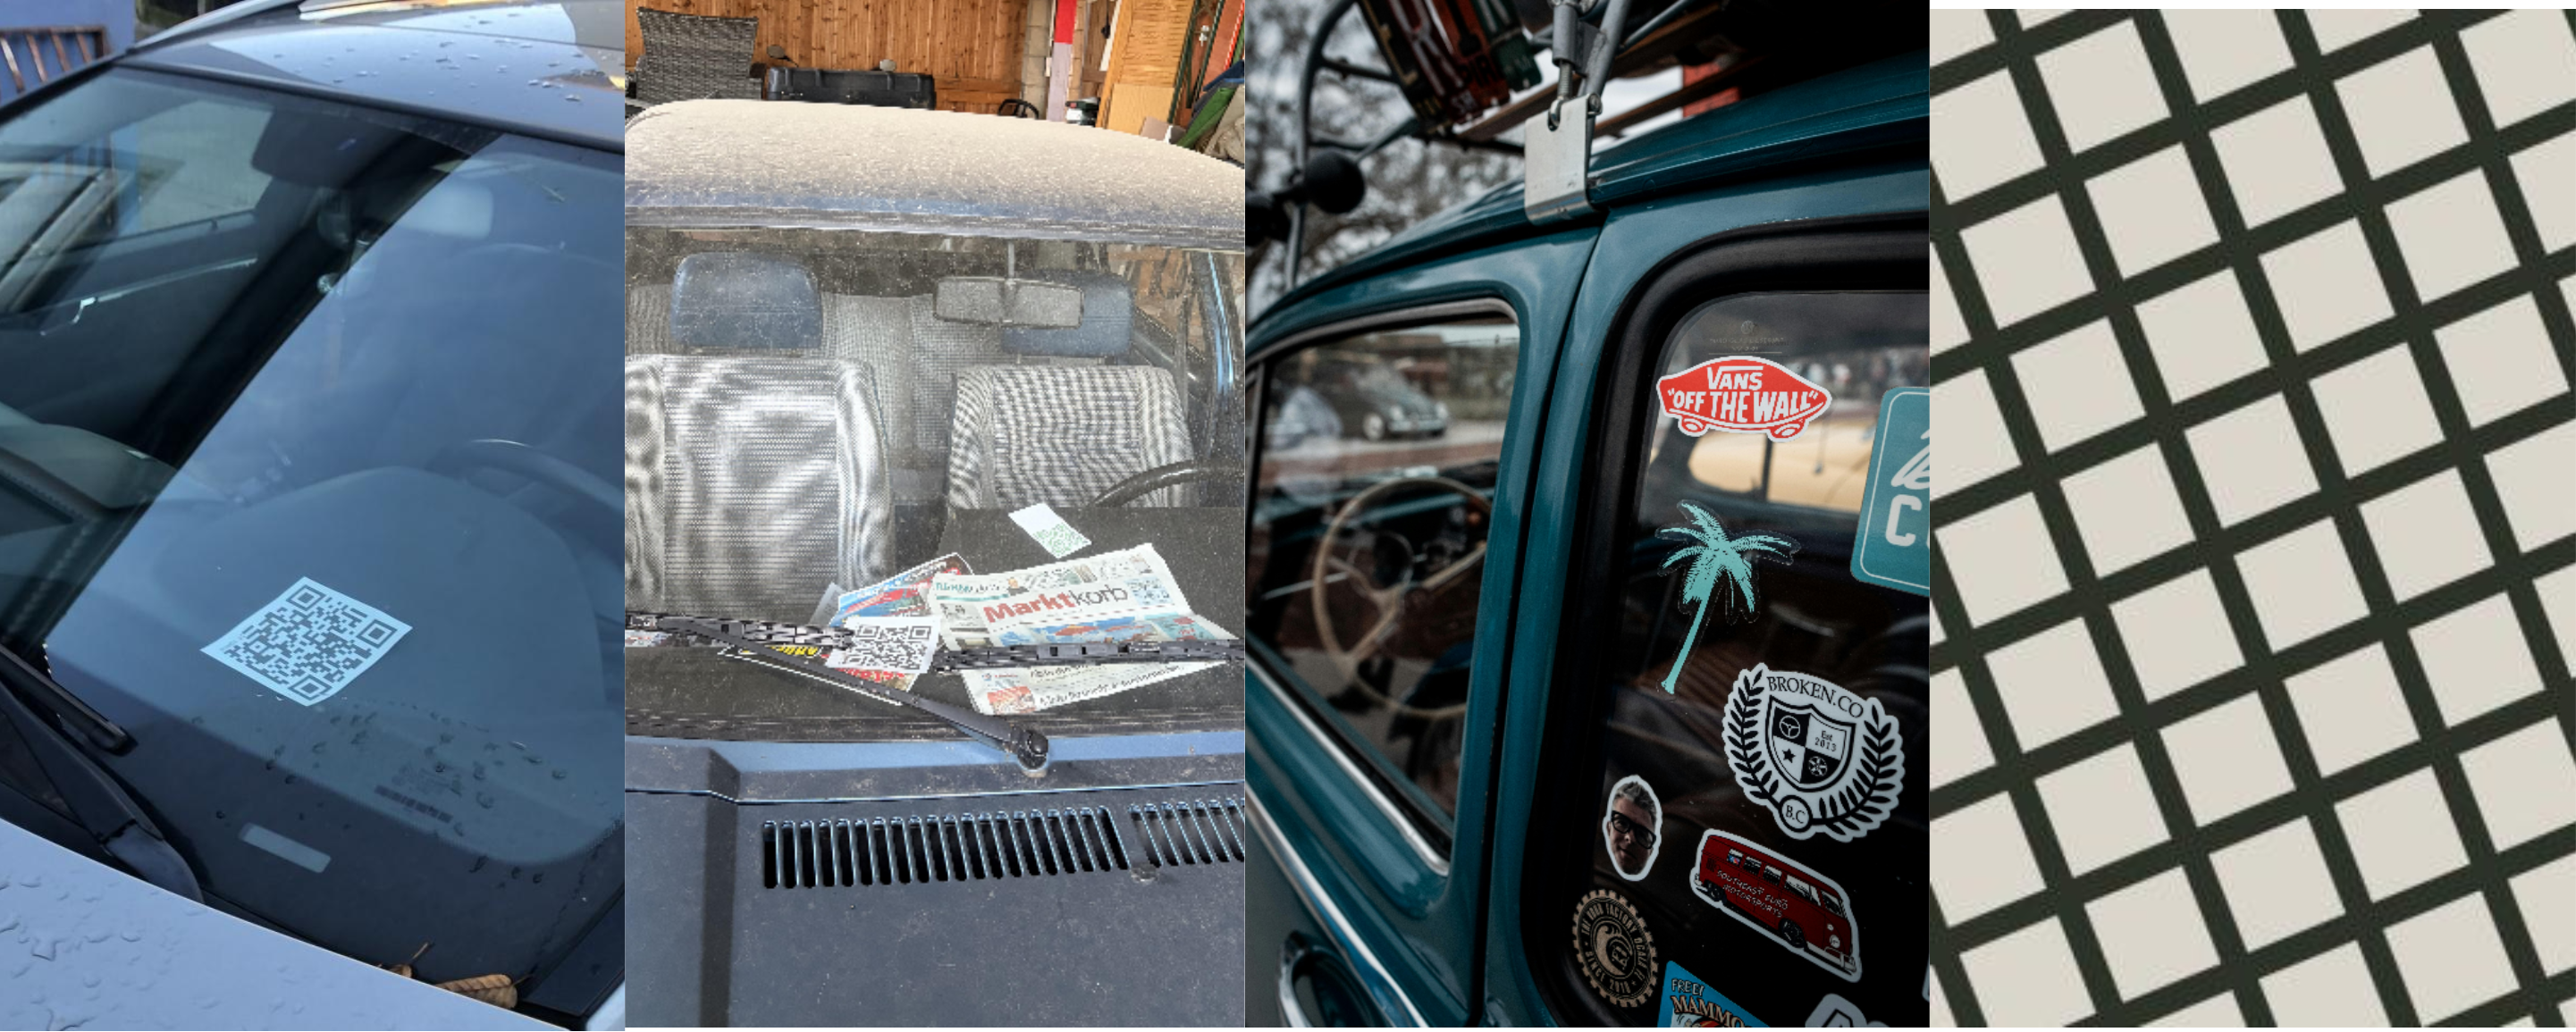
\includegraphics[width=1.0\textwidth]{Images/datenquellen.png}
    
    % [Kurzversion für Verzeichnis]{Lange Beschreibung unter dem Bild}
    \caption[Exemplarische Auszüge aus den Datenquellen]{Repräsentative Beispiele aus den vier genutzten Bildquellen (v.l.n.r.): (1) Kursmaterial aus Ilias, (2) Eigene Aufnahme, (3) Hintergrundbild (Pexels) und (4) Textur aus dem DTD-Datensatz.}
    
    % Label für die Referenzierung (Muss NACH caption stehen!)
    \label{fig:datenquellen}
\end{figure}

\subsection{Vorverarbeitung und Labeling} \label{subsec:vorverarbeitung_labeling}

Da die verwendeten Klassifikationsmodelle auf quadratische Eingaben (Patches) trainiert werden, müssen die aufgenommenen Vollbilder in das Format $256 \times 256$ Pixel überführt werden. Dieser Schritt ist entscheidend, um aus einer überschaubaren Anzahl an Vollbildern einen umfangreichen Trainingsdatensatz zu generieren.

\subsubsection{Evolution der Labeling-Strategie} \label{subsubsec:evolution_labeling}
In einer ersten Iteration wurde versucht, diesen Prozess manuell durchzuführen. Hierbei wurden mittels der im \autoref{subsec:roi_ansatz} beschriebenen RoI-Filter Kandidaten ausgeschnitten. Um \textit{Label Noise} zu vermeiden und die Qualität des Datensatzes zu maximieren, wurde ein Patch nur dann händisch als positiv gelabelt, wenn er alle folgenden drei Kriterien erfüllte:

\begin{enumerate}
    \item \textbf{Abdeckung:} Mindestens ca. \SI{30}{\percent} des QR-Codes müssen im Patch enthalten sein.
    \item \textbf{Geometrische Anker:} Mindestens eines der \textit{Finder Patterns} in den Ecken des Codes muss im Ausschnitt liegen.
    \item \textbf{Visuelle Validierung:} Das \textit{Finder Pattern} muss für das menschliche Auge klar als solches identifizierbar sein (hinreichende Schärfe und Kontrast).
\end{enumerate}

Eine besondere Bedeutung kam hierbei der Behandlung von Grenzfällen zu. Enthielt ein Patch zwar Fragmente eines QR-Codes (z.\,B. Datenpixel), verletzte aber eines der oben genannten Kriterien, wurde dieser Patch \textbf{komplett verworfen} und nicht als Negativ-Beispiel genutzt. Dies verhindert, dass das Modell widersprüchliche Informationen lernt (z.\,B. dass Pixelstrukturen, die eigentlich zu einem QR-Code gehören, der Negativ-Klasse zugeordnet werden).
Trotz dieser strengen Qualitätssicherung erwies sich der Ansatz als extrem zeitaufwendig. Es konnten so lediglich ca. 6.000 positive und 14.000 negative Patches generiert werden.

Um den Prozess zu skalieren, wurde die Strategie im Laufe des Projektes auf ein \textit{Bounding-Box-Labeling} umgestellt. Mithilfe des Tools \href{https://roboflow.com/}{\textit{Roboflow}} wurden in den Vollbildern Rechtecke um die relevanten Objekte gezeichnet. Dabei wurden zwei Kategorien definiert:
\begin{itemize}
    \item \textbf{QR-Code:} Der eigentlich zu erkennende Code (Positiv).
    \item \textbf{Distractor:} Visuelle Störobjekte, die einem QR-Code ähneln oder oft neben ihm auftreten (z.\,B. Plaketten, Parktickets, textreiche Kassenzettel).
\end{itemize}
Durch diesen effizienteren Workflow konnten in kurzer Zeit über 3.700 Vollbilder annotiert werden.

\subsubsection{Automatisierte Patch-Generierung} \label{subsubsec:automatische_patch_generierung}
Für die Erstellung der finalen Trainingsdaten wurde der bereits implementierte \textit{Multi-Scale Sliding Window}-Algorithmus wiederverwendet. Da durch den Roboflow-Export (PyTorch v5 Format) die Koordinaten aller Objekte im Vollbild bekannt waren, konnte das Ausschneiden und Labeln der Patches vollautomatisch erfolgen.

Das Skript schiebt das Fenster über das Bild und berechnet für jede Position Metriken relativ zu den gelabelten Bounding Boxes. Dabei wurden basierend auf der Konfigurationsdatei (\texttt{dataset\_config.yaml}) folgende Schwellenwerte angewendet:

\begin{itemize}
    \item \textbf{Positiv-Klasse:} Ein Patch wird als positiv gelabelt, wenn entweder die \textit{Coverage} (Anteil des Patches, der mit QR-Code gefüllt ist) \textbf{oder} das \textit{Containment} (Anteil des QR-Codes, der im Patch sichtbar ist) größer als \textbf{85\,\%} ist.
    
    \item \textbf{Ambiguous (Verworfen):} Liegt einer der Werte zwischen \textbf{10\,\%} und \textbf{85\,\%}, wird der Patch als ,,mehrdeutig`` eingestuft und komplett verworfen.
    
    \item \textbf{Hard Negative:} Enthält ein Patch zu mehr als \textbf{20\,\%} einen Distractor (z.\,B. Textblock), wird er gezielt als negatives Beispiel (textit{Hard Negative}) gespeichert.
    
    \item \textbf{Soft Negative (Hintergrund):} Enthält der Ausschnitt weder QR-Code noch Distractor, erfolgt eine Analyse der Bildstruktur. Liegt die Standardabweichung der Grauwerte unter \textbf{25}, wird der Patch als kontrastarm (\textit{Flat}) klassifiziert; andernfalls gilt er als strukturreich (\textit{Textured}).
\end{itemize}

\begin{figure}[H]
    \centering
    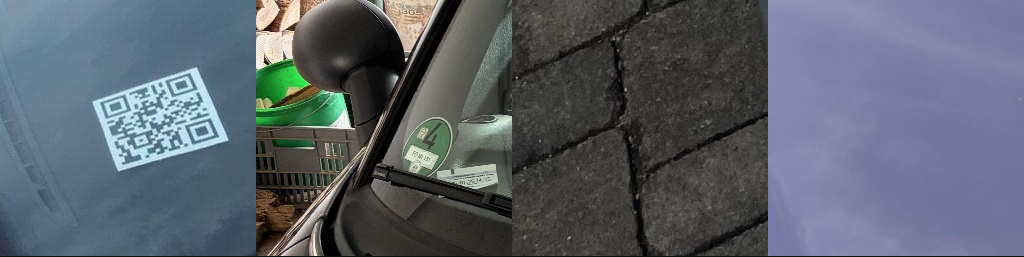
\includegraphics[width=1.0\textwidth]{Images/real_patches_types.png}
    
    % [Kurzversion für Verzeichnis]{Lange Beschreibung unter dem Bild}
    \caption[Exemplarische Darstellung der Patch-Kategorien]{Kategorisierung der generierten Trainingsdaten (v.l.n.r.): (1) Positiver Patch, (2) \textit{Hard Negative} mit \textit{Distractor}, (3) strukturreicher Hintergrund (\textit{Textured}) sowie (4) kontrastarmer Hintergrund (\textit{Flat}).}
    
    % Label für die Referenzierung (Muss NACH caption stehen!)
    \label{fig:patch_arten}
\end{figure}

\textbf{Begründung der strengen Filterung:}
Im Vergleich zum manuellen Labeling, bei dem bereits Fragmente akzeptiert wurden, setzen wir im automatisierten Prozess bewusst auf sehr hohe Schwellenwerte. Dies verfolgt zwei strategische Ziele:

\begin{enumerate}
    \item \textbf{Saubere Klassentrennung:} Das Verwerfen der \textit{Ambiguous}-Patches schafft eine klare Pufferzone. Das Modell soll lernen, signifikante QR-Code-Merkmale von Hintergrundstrukturen zu unterscheiden, anstatt durch halb angeschnittene Fragmente, die weder eindeutig positiv noch negativ sind, verwirrt zu werden.
    \item \textbf{Reserve für Augmentation:} Da die Basisdaten den QR-Code fast vollständig zeigen, schaffen wir die notwendige Reserve für aggressive \textit{Online Augmentations} während des späteren Trainings. Wir können dem Netz im Training starke geometrische Verzerrungen und Ausschnitte zumuten, ohne dass die Information verloren geht. Hätten wir bereits unvollständige Patches im Datensatz, würden diese durch eine weitere künstliche Augmentierung unkenntlich werden.
\end{enumerate}

\subsubsection{Resultierender Datensatz} \label{subsubsec:resultierender_datensatz}
Durch diese automatisierte \textit{Pipeline} konnte die Datenmenge im Vergleich zum manuellen Ansatz massiv gesteigert und gleichzeitig die Varianz erhöht werden. Der Datensatz, der aus realen Daten entstand, setzt sich wie folgt zusammen:

\begin{itemize}
    \item \textbf{ca. 15.286} positive Patches (QR-Code enthalten).
    \item \textbf{ca. 21.677} \textit{Hard Negatives} (\textit{Distractors} enthalten).
    \item \textbf{ca. 11.721} strukturreiche Hintergründe (hoher Kontrast, z.\,B. Wiese, Pflastersteine).
    \item \textbf{ca. 17.923} kontrastarme Hintergründe (wenig Information, z.\,B. Himmel, Lackflächen).
\end{itemize}

\subsection{Synthetische Daten} \label{subsec:synthetische_daten}

Obwohl der aus realen Aufnahmen gewonnene Datensatz bereits eine solide Basis bildet, ist er in seiner Varianz begrenzt. Bestimmte Randfälle – wie extrem verdrehte QR-Codes, spezifische Lichtreflexionen oder seltene Störobjekte – treten in den gesammelten Bildern nicht häufig genug auf, um vom Modell robust gelernt zu werden.
Um diese Lücken zu schließen und die Balance zwischen den Klassen flexibel steuern zu können, wurde eine \textit{Pipeline} zur Generierung synthetischer Daten entwickelt.

\subsubsection{Funktionsweise des Generators} \label{subsubsec:funktion_daten_generator}
Der implementierte Generator (\texttt{data\_generator.py}) erzeugt vollständig neue Trainingsbilder, indem er verschiedene Bildelemente nach dem Schichten-Prinzip stochastisch kombiniert. Ziel ist es, Patches zu erstellen, die realen Kameraaufnahmen so nahe wie möglich kommen, jedoch eine deutlich höhere Varianz aufweisen.

Der Prozess gliedert sich in drei Ebenen:

\begin{enumerate}
    \item \textbf{Hintergrund:}
    Als Basis dient ein zufällig gewählter Bildausschnitt. Hierbei greift der Generator zu gleichen Teilen auf zwei Quellen zurück:
    \begin{itemize}
        \item \textbf{Realwelt-Szenen:} Hochauflösende Bilder von Pexels (z.\,B. Straßenverkehr, Städte), aus denen mittels \textit{Sliding-Window}-Simulation zufällige Ausschnitte gewählt werden.
        \item \textbf{Texturen:} Bilder aus dem DTD-Datensatz, um das Modell gegen abstrakte Muster (Waben, Punkte, Geflechte) zu härten.
    \end{itemize}

    \item \textbf{Objekt-Platzierung:}
    Je nach Zielklasse wird ein Vordergrund-Objekt generiert und in den Hintergrund integriert:
    \begin{itemize}
        \item \textbf{Positiv-Klasse:} Es wird ein QR-Code mit zufälligem Inhalt erzeugt. Um die Realität abzubilden, wird dieser vielfältig modifiziert: Die geometrische Verzerrung simuliert Kamerawinkel (Perspektive), eine Rotation um $\pm \SI{180}{\degree}$ macht das Modell lageunabhängig, und Farb-Invertierungen oder Kratzer simulieren beschädigte Ausdrucke.
        Zusätzlich werden in ca. 60\,\% der Fälle noch \textit{vor} dem QR-Code weitere Störobjekte im Hintergrund platziert, um das Modell daran zu gewöhnen, den Code auch in ,,unaufgeräumten`` Szenen zu finden.

        \item \textbf{Hard Negatives (Distractors):} Um Fehlalarme zu minimieren, platziert der Generator gezielt Objekte, die einem QR-Code ähneln. Dazu zählen generierte \textit{Barcodes}, Versandlabels, zufällige Textblöcke sowie geometrische Formen. Eine besondere Herausforderung stellen hierbei zufällige Pixelmatrizen (\textit{Data Matrix}) dar, die einem QR-Code visuell stark ähneln, denen jedoch die charakteristischen \textit{Finder Patterns} fehlen.

    \end{itemize}

    \item \textbf{Integration und Effekte:}
    Damit das eingefügte Objekt nicht künstlich wirkt, wird es optisch mit dem Hintergrund verschmolzen. Dies geschieht durch Weichzeichnung (Simulation von Fokus-Unschärfe), Hinzufügen von ISO-Rauschen (Körnung) sowie die Simulation von Lichtreflexionen (\textit{Glare}) und Helligkeitsverläufen über das gesamte Bild.
\end{enumerate}

Durch diesen Ansatz können wir gezielt Szenarien trainieren, die in der Realität schwer zu erfassen sind (z.\,B. ein stark zerkratzter QR-Code bei schlechtem Licht), und so die Robustheit des finalen Modells signifikant steigern.

\begin{figure}[H]
    \centering
    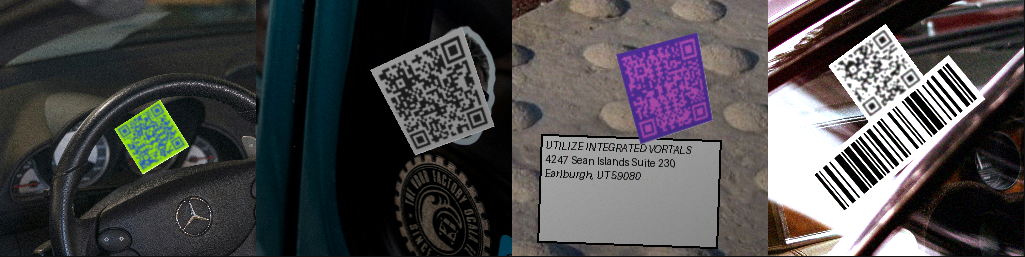
\includegraphics[width=1.0\textwidth]{Images/synthetic_pos_patches.png}
    
    % [Kurzversion für Verzeichnis]{Lange Beschreibung unter dem Bild}
    \caption[Synthetische Beispiele der Positiv-Klasse]{Synthetisch generierte Beispiele der Positiv-Klasse. Die Patches demonstrieren die hohe Varianz durch Rotation, Farbgebung und simulierte Unschärfe sowie die Integration von zusätzlichen \textit{Distractors} im Hintergrund.}
    
    % Label für die Referenzierung (Muss NACH caption stehen!)
    \label{fig:syn_pos_patches}
\end{figure}

\begin{figure}[H]
    \centering
    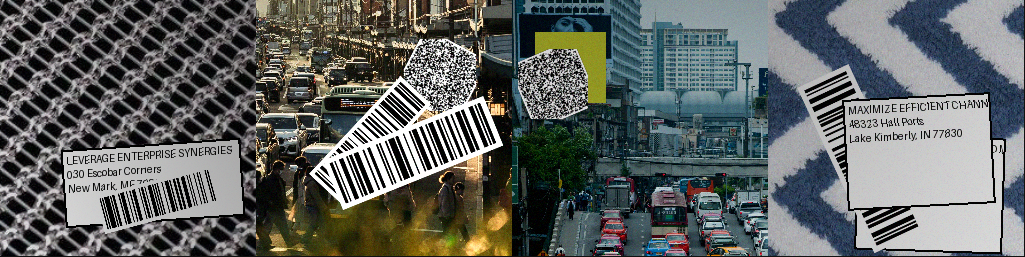
\includegraphics[width=1.0\textwidth]{Images/synthetic_neg_patches.png}
    
    % [Kurzversion für Verzeichnis]{Lange Beschreibung unter dem Bild}
    \caption[Synthetische Beispiele der Negativ-Klasse]{Synthetisch generierte Beispiele der Negativ-Klasse. Zu sehen sind typische \textit{Distractors} (\textit{Hard Negatives}) wie \textit{Barcodes}, Textfragmente oder geometrische Formen, die vor variierenden Hintergründen platziert wurden.}
    
    % Label für die Referenzierung (Muss NACH caption stehen!)
    \label{fig:syn_neg_patches}
\end{figure}

\subsection{Finaler Datensatz} \label{subsec:finaler_datensatz}

Der finale Datensatz für das Training der neuronalen Netze entsteht durch die Fusion der bereinigten realen Aufnahmen mit den generierten synthetischen Daten. Ziel war es, eine Gesamtmenge von 100.000 Patches zu erreichen, wobei ein bewusstes Ungleichgewicht zwischen den Klassen angestrebt wurde.

\subsubsection{Zusammensetzung und Klassenbalance}
Die Verteilung zwischen der Positiv- und der Negativ-Klasse wurde auf ein Verhältnis von \textbf{1:3} festgelegt (25.000 zu 75.000 Patches). Diese Entscheidung leitet sich direkt aus der späteren Anwendung im \textit{Sliding-Window}-Verfahren ab:
Da das Fenster im realen Betrieb in hunderten Schritten über das Bild gleitet, sieht das Modell statistisch gesehen überwiegend Hintergrund (Negativ-Beispiele) und nur sehr selten einen QR-Code. Um die Rate an Fehlalarmen (\textit{False Positives}) effektiv zu minimieren, muss das Netz daher besonders intensiv darauf trainiert werden, verschiedenste Formen von Hintergrund und Störobjekten sicher als negativ zu klassifizieren.

Um diese Zielgrößen zu erreichen, wurden die vorhandenen realen Daten mit synthetischen Patches aufgefüllt. Dies erhöht nicht nur die Quantität, sondern reichert den Datensatz gezielt mit Randfällen an, die in den realen Daten unterrepräsentiert waren.

\begin{table}[H]
    \centering
    \caption{Zusammensetzung des finalen Datensatzes}
    \label{tab:final_dataset}
    \begin{tabular}{llrlp{5cm}}
        \toprule
        \textbf{Klasse} & \textbf{Quelle} & \textbf{Anzahl} & \textbf{Gesamt} & \textbf{Anmerkung} \\
        \midrule
        \textbf{Positiv} & Real & 15.286 & \textbf{25.000} & 61\,\% Realanteil \\
         & Synthetisch & 9.714 & & Ergänzt seltene Perspektiven, Blendeffekte, und \textit{Distractors}. \\
        \midrule
        \textbf{Negativ} & Real & 51.321 & \textbf{75.000} & 68\,\% Realanteil \\
         & Synthetisch & 23.679 & & Ergänzt verschiedene kontrast- und struktureiche Hintergründe sowie Hard Negatives mit Distractors. \\
        \bottomrule
    \end{tabular}
\end{table}

\subsubsection{Daten-Split (\textit{Train} / \textit{Validierung} / \textit{Test})}
Für das Training wurde der Gesamtdatensatz in drei Teilmengen unterteilt. Die Aufteilung erfolgte im Verhältnis \textbf{90\,\% Training}, \textbf{9,8\,\% Validierung} und \textbf{0,2\,\% Test}.

\begin{itemize}
    \item \textbf{Training (90.000 Patches):} Der Großteil der Daten wird genutzt, um die Gewichte des Modells zu optimieren.
    \item \textbf{Validierung (9.800 Patches):} Dieser Teil dient dazu, während des Trainings die Leistung zu überwachen und Hyperparameter zu optimieren. Knapp 10.000 Bilder reichen aus, um eine statistisch stabile Aussage über die Generalisierungsfähigkeit des Modells zu treffen.
    \item \textbf{Test (200 Patches):} Ein kleiner, unberührter Datensatz für eine finale Funktionsprüfung der Klassifikation vor der Integration.
\end{itemize}

\section{Eigenes Convolutional Neural Network} \label{sec:eigenes_cnn}

Im folgenden Abschnitt wird die Entwicklung und Architektur des eigens entworfenen \textit{Convolutional Neural Networks} (CNN) vorgestellt. Die zentrale Anforderung an dieses Modell ergibt sich direkt aus dem gewählten \textit{Sliding-Window}-Ansatz: Da für jedes einzelne Vollbild der Kamera hunderte von Patches klassifiziert werden müssen, ist eine extrem geringe Inferenzzeit essenziell. Der Fokus lag daher auf dem Entwurf einer ,,\textit{Lightweight}``-Architektur mit möglichst wenigen trainierbaren Parametern, um eine flüssige Verarbeitung zu gewährleisten.

Eine grundlegende Designentscheidung ist hierbei die Verwendung von Graustufenbildern. Da ein QR-Code technisch durch binäre Kontraste und spezifische geometrische Anker definiert ist, bietet Farbinformation nur begrenzt einen Mehrwert für die Klassifikation. Im Gegenteil: Durch die Reduktion auf einen einzigen Farbkanal wird die Eingabekomplexität verringert und das Netz gezwungen, sich auf strukturelle Merkmale – wie Kantenübergänge und \textit{Finder Patterns} – zu konzentrieren, anstatt irrelevante Farbvariationen zu lernen.

Es ist zu beachten, dass die Entwicklung des Modells kein linearer, sondern ein iterativer Prozess war. Der im vorangegangenen Kapitel beschriebene finale Datensatz stand nicht von Beginn an in dieser Qualität zur Verfügung. Vielmehr haben sich Netzarchitektur und Datengrundlage in parallelen Zyklen weiterentwickelt. Auf diese evolutionäre Wechselwirkung zwischen Modelloptimierung und Datenverbesserung wird in den nachfolgenden Unterkapiteln explizit eingegangen.

\subsection{Experimentelle Entwicklung} \label{subsec:experimentelle_entwicklung_cnn}

Die Entwicklung des eigenen CNN-Modells erfolgte in einem iterativen Prozess über insgesamt sieben Stufen. In jedem Schritt wurden basierend auf der Analyse der vorherigen Ergebnisse gezielt Hyperparameter angepasst, die Architektur verfeinert oder die Datengrundlage erweitert.
Im Folgenden wird dieser Entwicklungsprozess chronologisch dokumentiert.

% ==========================================
% ITERATION 1 (BASELINE)
% ==========================================
\subsubsection{Iteration 1: Baseline CNN} \label{subsubsec:iter1}

\textbf{Zielsetzung:} Etablierung einer ersten Referenz (\textit{Baseline}) mit einer kompakten ,,\textit{Lightweight}``-Architektur, um die grundsätzliche Lernfähigkeit auf dem Datensatz zu prüfen.

% 1. Hyperparameter Tabelle
\begin{table}[H]
    \centering
    \caption{Hyperparameter Iteration 1 (\textit{Baseline})}
    \label{tab:hyperparams_iter1}
    \begin{tabular}{ll}
        \toprule
        \textbf{Parameter} & \textbf{Wert} \\
        \midrule
        \textit{Batch Size} & 32 \\
        \textit{Epochs} & 50 \\
        \textit{Learning Rate} & 0,001 \\
        \textit{Optimizer} & Adam \\
        \textit{Loss Function} & \textit{Binary Crossentropy} \\
        \bottomrule
    \end{tabular}
\end{table}

% Callbacks Tabelle
\begin{table}[H]
    \centering
    \caption{Verwendete \textit{Callbacks} und Parameter in Iteration 1}
    \label{tab:callbacks_iter1}
    \begin{tabular}{lll}
        \toprule
        \textbf{Callback} & \textbf{Parameter} & \textbf{Wert} \\
        \midrule
        \textit{EarlyStopping}     & Monitor & val\_loss \\
                          & \textit{Patience} & 5 \\
                          & \textit{Restore Best Weights} & \texttt{True} \\
        \bottomrule
    \end{tabular}
\end{table}

% 2. Modell Summary Tabelle
\begin{table}[H]
    \centering
    \caption{Modellarchitektur Iteration 1}
    \label{tab:model_summary_iter1}
    \begin{tabular}{llr}
        \toprule
        \textbf{Layer (type)} & \textbf{Output Shape} & \textbf{Param \#} \\
        \midrule
        InputLayer & (None, 256, 256, 1) & 0 \\
        Conv2D (relu) & (None, 256, 256, 32) & 320 \\
        BatchNormalization & (None, 256, 256, 32) & 128 \\
        MaxPooling2D & (None, 128, 128, 32) & 0 \\
        Conv2D (relu) & (None, 128, 128, 64) & 18.496 \\
        BatchNormalization & (None, 128, 128, 64) & 256 \\
        MaxPooling2D & (None, 64, 64, 64) & 0 \\
        Conv2D (relu) & (None, 64, 64, 128) & 73.856 \\
        MaxPooling2D & (None, 32, 32, 128) & 0 \\
        GlobalAveragePooling2D & (None, 128) & 0 \\
        Dense (relu) & (None, 128) & 16.512 \\
        Dropout (0.5) & (None, 128) & 0 \\
        Dense (sigmoid) & (None, 1) & 129 \\
        \midrule
        \textbf{Total params} & & \textbf{109.697} \\
        \textbf{Trainable params} & & \textbf{109.505} \\
        \textbf{Non-trainable params} & & \textbf{192} \\
        \bottomrule
    \end{tabular}
\end{table}

% 3. Datensatz Zustand
\textbf{Datengrundlage:}
Zum Zeitpunkt dieser ersten Iteration befand sich der Datensatz noch in einem frühen Entwicklungsstadium. Verwendet wurde ein Mischbestand aus manuell gelabelten realen Aufnahmen und ersten synthetisch generierten Daten. Die Zusammensetzung gestaltete sich wie folgt:
\begin{itemize}
    \item \textbf{Positiv-Klasse:} ca. 3.000 reale und 17.000 synthetische Patches.
    \item \textbf{Negativ-Klasse:} ca. 12.000 reale und 8.000 synthetische Patches.
\end{itemize}
Es ist anzumerken, dass der Generator für die synthetischen Daten in dieser Phase noch Qualitätsmängel aufwies. Dies führte teilweise zu Artefakten oder QR-Codes, die visuell kaum erkennbar waren, was eine zusätzliche Rauschkomponente in das Training einbrachte.

% 4. Trainingsverlauf Bild
\begin{figure}[H]
    \centering
    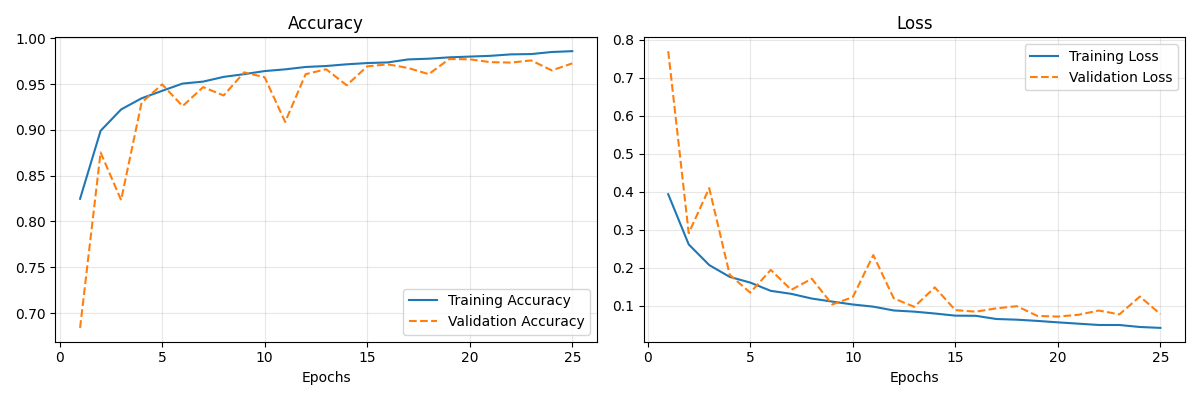
\includegraphics[width=1.0\textwidth]{Images/Custom/Iteration_1/training_metrics.png}
    \caption[Trainingsverlauf Iteration 1]{Verlauf von Loss und Accuracy über die Epochen in Iteration 1.}
    \label{fig:history_custom_iter1}
\end{figure}

% 6. Metriken Tabelle
\begin{table}[H]
    \centering
    \caption{Ergebnisse Iteration 1, beste Epoche: 20}
    \label{tab:results_iter1}
    \begin{tabular}{cccc}
        \toprule
        \textbf{Train Loss} & \textbf{Val Loss} & \textbf{Train Acc} & \textbf{Val Acc} \\
        \midrule
        0,057 & 0,0721 & 97,99\,\% & 97,70\,\% \\
        \bottomrule
    \end{tabular}
\end{table}

% 7. Analyse
\textbf{Analyse:}
Die Ergebnisse der \textit{Baseline-Iteration} sind überraschend positiv. Trotz der beschriebenen Mängel in den synthetischen Daten und der simplen Modellarchitektur erreicht das Netz bereits eine Validierungsgenauigkeit von über 97\,\%.

Besonders bemerkenswert ist der geringe Unterschied zwischen \textit{Train Acc} (97,99\,\%) und \textit{Val Acc} (97,70\,\%). Dies deutet darauf hin, dass unter den gegebenen Bedingungen (noch) kein signifikantes \textit{Overfitting} stattfindet. Das Modell scheint erfolgreich grundlegende geometrische Merkmale (wie die \textit{Finder Patterns}) zu generalisieren, anstatt die begrenzten realen Trainingsdaten auswendig zu lernen. Dass die beste Leistung bereits in Epoche 20 erreicht wurde, bestätigt zudem die Hypothese, dass die kompakte Architektur eine schnelle Konvergenz ermöglicht. Diese Iteration dient somit als erfolgreicher ,,\textit{Proof of Concept}``.

% ==========================================
% ITERATION 2 (Stabilisierung)
% ==========================================
\subsubsection{Iteration 2: Stabilisierung und Learning Rate Scheduling} \label{subsubsec:iter2}

\textbf{Zielsetzung:} Nachdem die \textit{Baseline} eine hohe Genauigkeit, aber einen teilweise instabilen Trainingsverlauf zeigte, lag der Fokus dieser Iteration auf der Stabilisierung. Durch Anpassung der \textit{Learning Rate} und Erweiterung der Normalisierung sollten \textit{Loss-Spikes} verhindert und die Konvergenz geglättet werden.

% 1. Hyperparameter Tabelle
\begin{table}[H]
    \centering
    \caption{Hyperparameter Iteration 2}
    \label{tab:hyperparams_iter2}
    \begin{tabular}{ll}
        \toprule
        \textbf{Parameter} & \textbf{Wert} \\
        \midrule
        \textit{Batch Size} & 32 \\
        \textit{Epochs} & 50 \\
        \textbf{\textit{Learning Rate}} & 0,001 $\rightarrow$ \textbf{0,0001} \\
        \textit{Optimizer} & Adam \\
        \textit{Loss Function} & \textit{Binary Crossentropy} \\
        \bottomrule
    \end{tabular}
\end{table}

% Callbacks Tabelle Iteration 2
\begin{table}[H]
    \centering
    \caption{Verwendete \textit{Callbacks} und Parameter in Iteration 2}
    \label{tab:callbacks_iter2}
    \begin{tabular}{lll}
        \toprule
        \textbf{Callback} & \textbf{Parameter} & \textbf{Wert} \\
        \midrule
        \textbf{\textit{ReduceLROnPlateau}} & \textit{Monitor} & \texttt{val\_loss} \\
                                   & \textit{Factor} & \textbf{0,5} \\
                                  & \textit{Patience} & \textbf{2} \\
                                  & \textit{Min LR} & $\mathbf{10^{-6}}$ \\
        \midrule
        \textit{EarlyStopping}     & \textit{Monitor} & \texttt{val\_loss} \\
                                  & \textit{Patience} & 5 \\
                                  & \textit{Restore Best Weights} & \texttt{True} \\
        \bottomrule
    \end{tabular}
\end{table}

% 2. Modell Summary Tabelle (Batch Norm fett)
\begin{table}[H]
    \centering
    \caption{Modellarchitektur Iteration 2 (angepasst)}
    \label{tab:model_summary_iter2}
    \begin{tabular}{llr}
        \toprule
        \textbf{Layer (type)} & \textbf{Output Shape} & \textbf{Param \#} \\
        \midrule
        InputLayer & (None, 256, 256, 1) & 0 \\
        Conv2D (relu) & (None, 256, 256, 32) & 320 \\
        BatchNormalization & (None, 256, 256, 32) & 128 \\
        MaxPooling2D & (None, 128, 128, 32) & 0 \\
        Conv2D (relu) & (None, 128, 128, 64) & 18.496 \\
        BatchNormalization & (None, 128, 128, 64) & 256 \\
        MaxPooling2D & (None, 64, 64, 64) & 0 \\
        Conv2D (relu) & (None, 64, 64, 128) & 73.856 \\
        \textbf{BatchNormalization} & (None, 64, 64, 128) & \textbf{512} \\
        MaxPooling2D & (None, 32, 32, 128) & 0 \\
        GlobalAveragePooling2D & (None, 128) & 0 \\
        Dense (relu) & (None, 128) & 16.512 \\
        Dropout (0,5) & (None, 128) & 0 \\
        Dense (sigmoid) & (None, 1) & 129 \\
        \midrule
        \textbf{Total params} & & \textbf{110.209} \\
        \textbf{Trainable params} & & \textbf{109.761} \\
        \textbf{Non-trainable params} & & \textbf{448} \\
        \bottomrule
    \end{tabular}
\end{table}

% 3. Datensatz Zustand
\textbf{Datengrundlage:}
Der Anteil der realen Trainingsdaten wurde leicht erhöht, sodass nun ca. 4.000 reale \textit{Patches} in den Datensatz einfließen. Das Verhältnis zu den synthetischen Daten wurde entsprechend angepasst, um die Balance zu wahren.

% 4. Hypothese
\textbf{Hypothese:}
Die signifikante Reduktion der \textit{Learning Rate} (von $10^{-3}$ auf $10^{-4}$) in Kombination mit dem dynamischen \textit{Scheduler} soll das ,,Oszillieren`` des \textit{Losses} minimieren. Die zusätzliche \textit{Batch Normalization} im tiefsten \textit{Layer} soll helfen, die Gradienten besser zu propagieren und das Training gegen die höhere Varianz der realen Daten zu stabilisieren.

% 5. Trainingsverlauf Bild
\begin{figure}[H]
    \centering
    
\includegraphics[width=1.0\textwidth]{Images/Custom/Iteration_2/training_metrics.png}
    \caption[Trainingsverlauf Iteration 2]{Verlauf von \textit{Loss} und \textit{Accuracy} in Iteration 2. Die Kurven verlaufen deutlich glatter als in der \textit{Baseline}.}
    \label{fig:history_custom_iter2}
\end{figure}

% 6. Metriken Tabelle
\begin{table}[H]
    \centering
    \caption{Ergebnisse Iteration 2, beste Epoche: 41}
    \label{tab:results_iter2}
    \begin{tabular}{cccc}
        \toprule
        \textbf{Train Loss} & \textbf{Val Loss} & \textbf{Train Acc} & \textbf{Val Acc} \\
        \midrule
        0,1170 & 0,1225 & 95,63\,\% & 95,17\,\% \\
        \bottomrule
    \end{tabular}
\end{table}

% 7. Analyse
\textbf{Analyse:}
Die Maßnahmen zur Stabilisierung waren erfolgreich: Die Lernkurve zeigt deutlich weniger Ausreißer (\textit{Spikes}) als in der ersten Iteration. Allerdings ging diese erhöhte Stabilität mit einer leichten Einbuße bei der Spitzenleistung einher. Die \textit{Validation Accuracy} sank im Vergleich zur \textit{Baseline} leicht auf ca. 95,2\,\%.
Dies ist ein typischer \textit{Trade-off}: Das Modell lernt nun ,,vorsichtiger`` und generalisiert robuster, erreicht aber (noch) nicht wieder die extrem hohen Werte des aggressiveren Trainings der \textit{Baseline}. Der geringe Abstand zwischen \textit{Training-} und \textit{Validation-Loss} zeigt jedoch, dass das Modell sehr gut generalisiert und kein \textit{Overfitting} vorliegt.

% ==========================================
% ITERATION 3 (Deep CNN und Flatten)
% ==========================================
\subsubsection{Iteration 3: Deep CNN und Flattening} \label{subsubsec:iter3}

\textbf{Zielsetzung:} Um komplexere Merkmale lernen zu können, wurde die Architektur grundlegend vertieft. Der Wechsel zu einem \textit{Deep CNN} mit 5 \textit{Convolutional Blocks} soll die \textit{Feature-Extraktion} verbessern. Gleichzeitig wurde das \textit{Global Average Pooling} durch einen \textit{Flatten}-Layer ersetzt, um räumliche Informationen aus den tieferen Schichten besser zu erhalten.

% 1. Hyperparameter Tabelle
\begin{table}[H]
    \centering
    \caption{Hyperparameter Iteration 3}
    \label{tab:hyperparams_iter3}
    \begin{tabular}{ll}
        \toprule
        \textbf{Parameter} & \textbf{Wert} \\
        \midrule
        \textit{Batch Size} & 32 \\
        \textit{Epochs} & 50 \\
        \textbf{\textit{Learning Rate}} & 0,0001 $\rightarrow$ \textbf{0,0005} \\
        \textit{Optimizer} & Adam \\
        \textit{Loss Function} & \textit{Binary Crossentropy} \\
        \bottomrule
    \end{tabular}
\end{table}

% Callbacks Tabelle Iteration 3
\begin{table}[H]
    \centering
    \caption{Verwendete \textit{Callbacks} und Parameter in Iteration 3}
    \label{tab:callbacks_iter3}
    \begin{tabular}{lll}
        \toprule
        \textbf{Callback} & \textbf{Parameter} & \textbf{Wert} \\
        \midrule
        \textit{ReduceLROnPlateau} & \textit{Monitor} & \texttt{val\_loss} \\
                          & \textit{Factor} & 0,5 \\
                          & \textbf{\textit{Patience}} & 2 $\rightarrow$ \textbf{3} \\
                          & \textit{Min LR} & $10^{-6}$ \\
        \midrule
        \textit{EarlyStopping}     & \textit{Monitor} & \texttt{val\_loss} \\
                          & \textbf{\textit{Patience}} & 5 $\rightarrow$ \textbf{8} \\
                          & \textit{Restore Best Weights} & \texttt{True} \\
        \bottomrule
    \end{tabular}
\end{table}

% 2. Modell Summary Tabelle
\begin{table}[H]
    \centering
    \caption{Modellarchitektur Iteration 3 (\textit{Deep CNN})}
    \label{tab:model_summary_iter3}
    \begin{tabular}{llr}
        \toprule
        \textbf{Layer (type)} & \textbf{Output Shape} & \textbf{Param \#} \\
        \midrule
        InputLayer & (None, 256, 256, 1) & 0 \\
        Conv2D (relu) & (None, 256, 256, 32) & 320 \\
        BatchNormalization & (None, 256, 256, 32) & 128 \\
        MaxPooling2D & (None, 128, 128, 32) & 0 \\
        Conv2D (relu) & (None, 128, 128, 64) & 18.496 \\
        BatchNormalization & (None, 128, 128, 64) & 256 \\
        MaxPooling2D & (None, 64, 64, 64) & 0 \\
        Conv2D (relu) & (None, 64, 64, 128) & 73.856 \\
        BatchNormalization & (None, 64, 64, 128) & 512 \\
        MaxPooling2D & (None, 32, 32, 128) & 0 \\
        % NEUE BLÖCKE
        \textbf{Conv2D (relu)} & (None, 32, 32, 128) & \textbf{147.584} \\
        \textbf{BatchNormalization} & (None, 32, 32, 128) & \textbf{512} \\
        \textbf{MaxPooling2D} & (None, 16, 16, 128) & \textbf{0} \\
        \textbf{Conv2D (relu)} & (None, 16, 16, 128) & \textbf{147.584} \\
        \textbf{BatchNormalization} & (None, 16, 16, 128) & \textbf{512} \\
        \textbf{MaxPooling2D} & (None, 8, 8, 128) & \textbf{0} \\
        % FLATTEN statt GAP
        \textbf{Flatten} & (None, 8192) & \textbf{0} \\
        \textbf{Dense (relu)} & (None, 64) & \textbf{524.352} \\
        Dropout (0,5) & (None, 64) & 0 \\
        Dense (sigmoid) & (None, 1) & 65 \\
        \midrule
        \textbf{Total params} & & \textbf{914.177} \\
        \textbf{Trainable params} & & \textbf{913.217} \\
        \textbf{Non-trainable params} & & \textbf{968} \\
        \bottomrule
    \end{tabular}
\end{table}

% 3. Datensatz Zustand
\textbf{Datengrundlage:}
Die Datengrundlage blieb gegenüber Iteration 2 unverändert. Der Fokus dieser Iteration lag rein auf der Optimierung der Modellarchitektur und der Hyperparameter, um die Leistung auf dem bestehenden Datensatz (ca. 4.000 reale \textit{Patches}, ergänzt durch synthetische Daten) zu maximieren.

% 4. Hypothese
\textbf{Hypothese:}
Das tiefere Netzwerk mit 5 Blöcken sollte in der Lage sein, komplexere und abstraktere Merkmale des QR-Codes zu lernen, die einem flacheren Netz verborgen bleiben. Der Ersatz von \textit{Global Average Pooling} durch \textit{Flattening} zielt darauf ab, die räumliche Information der \textit{Feature-Maps} (8x8) direkt in den \textit{Dense-Layer} zu übertragen, was bei geometrischen Objekten wie QR-Codes von Vorteil sein kann. Die Erhöhung der \textit{Learning Rate} auf 0,0005 soll die Konvergenz des nun deutlich parameterreicheren Modells (ca. 1 Mio. Parameter) beschleunigen.

% 5. Trainingsverlauf Bild
\begin{figure}[H]
    \centering
    
\includegraphics[width=1.0\textwidth]{Images/Custom/Iteration_3/training_metrics.png}
    \caption[Trainingsverlauf Iteration 3]{Verlauf von \textit{Loss} und \textit{Accuracy} in Iteration 3. Zu erkennen ist ein schneller Anstieg der Genauigkeit, gefolgt von Instabilitäten.}
    \label{fig:history_custom_iter3}
\end{figure}

% 6. Metriken Tabelle
\begin{table}[H]
    \centering
    \caption{Ergebnisse Iteration 3, beste Epoche: 12}
    \label{tab:results_iter3}
    \begin{tabular}{cccc}
        \toprule
        \textbf{Train Loss} & \textbf{Val Loss} & \textbf{Train Acc} & \textbf{Val Acc} \\
        \midrule
        0,0300 & 0,0994 & 98,90\,\% & 97,10\,\% \\
        \bottomrule
    \end{tabular}
\end{table}

% 7. Analyse
\textbf{Analyse:}
Die Ergebnisse bestätigen die Leistungsfähigkeit der tieferen Architektur: Bereits in Epoche 5 wurde eine \textit{Validation Accuracy} von ca. 96,0\,\% erreicht, was den Spitzenwert der vorherigen Iteration übertrifft.
Jedoch zeigte sich im weiteren Verlauf eine signifikante Instabilität. Nach dem schnellen Anstieg wurde ein starkes \textit{Overfitting} beobachtet, bei dem der \textit{Training Loss} weiter sank (auf unter 0,03), während der \textit{Validation Loss} ab Epoche 6 dramatisch anstieg (\textit{Spike} auf bis zu 0,37).
Zwar erholte sich das Modell dank der \textit{Callbacks} wieder und erreichte in Epoche 12 seinen Bestwert (97,1\,\%), doch die hohe Varianz im \textit{Validation Loss} deutet darauf hin, dass das Modell dazu neigt, die Trainingsdaten auswendig zu lernen. Es wird deutlich, dass die gesteigerte Modellkapazität (ca. 1 Mio. Parameter) stärkere Regularisierungsmaßnahmen erfordert, um stabil zu generalisieren.

% ==========================================
% ITERATION 4 (Online Data Augmentation)
% ==========================================
\subsubsection{Iteration 4: Online Data Augmentation} \label{subsubsec:iter4}

\textbf{Zielsetzung:} Um dem beobachteten \textit{Overfitting} entgegenzuwirken und das Modell gegen reale Störungen zu härten, wurde die Strategie von einer statischen (\textit{Offline}) zu einer dynamischen (\textit{Online}) \textit{Data Augmentation} gewechselt. Anstatt feste Bilder zu generieren, werden die Trainingsdaten nun während des Trainings \textit{live} auf der GPU verfremdet. Dies erzeugt effektiv einen unendlichen Datensatz, da das Modell niemals exakt dasselbe Bild zweimal sieht.

% 1. Hyperparameter Tabelle
\begin{table}[H]
    \centering
    \caption{Hyperparameter Iteration 4}
    \label{tab:hyperparams_iter4}
    \begin{tabular}{ll}
        \toprule
        \textbf{Parameter} & \textbf{Wert} \\
        \midrule
        \textbf{\textit{Batch Size}} & 32 $\rightarrow$ \textbf{64} \\
        \textit{Epochs} & 50 \\
        \textit{Learning Rate} & 0,0005 \\
        \textit{Optimizer} & Adam \\
        \textit{Loss Function} & \textit{Binary Crossentropy} \\
        \bottomrule
    \end{tabular}
\end{table}

% Callbacks Tabelle Iteration 4
\begin{table}[H]
    \centering
    \caption{Verwendete \textit{Callbacks} und Parameter in Iteration 4}
    \label{tab:callbacks_iter4}
    \begin{tabular}{lll}
        \toprule
        \textbf{Callback} & \textbf{Parameter} & \textbf{Wert} \\
        \midrule
        \textit{ReduceLROnPlateau} & \textit{Monitor} & \texttt{val\_loss} \\
                          & \textit{Factor} & 0,5 \\
                          & \textbf{\textit{Patience}} & 3 $\rightarrow$ \textbf{4} \\
                          & \textit{Min LR} & $10^{-6}$ \\
        \midrule
        \textit{EarlyStopping}     & \textit{Monitor} & \texttt{val\_loss} \\
                          & \textbf{\textit{Patience}} & 8 $\rightarrow$ \textbf{10} \\
                          & \textit{Restore Best Weights} & \texttt{True} \\
        \bottomrule
    \end{tabular}
\end{table}

% 2. Modell Summary Tabelle (Augmentation Layer fett)
\begin{table}[H]
    \centering
    \caption{Modellarchitektur Iteration 4 (mit \textit{Online Augmentation})}
    \label{tab:model_summary_iter4}
    \begin{tabular}{llr}
        \toprule
        \textbf{Layer (type)} & \textbf{Output Shape} & \textbf{Param \#} \\
        \midrule
        InputLayer & (None, 256, 256, 1) & 0 \\
        % NEUE AUGMENTATION LAYER
        \textbf{\texttt{RandomFlip}} & (None, 256, 256, 1) & \textbf{0} \\
        \textbf{\texttt{RandomRotation (0,2)}} & (None, 256, 256, 1) & \textbf{0} \\
        \textbf{\texttt{RandomZoom (0,1)}} & (None, 256, 256, 1) & \textbf{0} \\
        \textbf{\texttt{RandomTranslation (0,1)}} & (None, 256, 256, 1) & \textbf{0} \\
        \textbf{\texttt{GaussianNoise (0,1)}} & (None, 256, 256, 1) & \textbf{0} \\
        \textbf{\texttt{RandomContrast (0,2)}} & (None, 256, 256, 1) & \textbf{0} \\
        \textbf{\texttt{Rescaling} (1/255)} & (None, 256, 256, 1) & \textbf{0} \\
        % BESTEHENDE ARCHITEKTUR
        Conv2D (relu) & (None, 256, 256, 32) & 320 \\
        BatchNormalization & (None, 256, 256, 32) & 128 \\
        MaxPooling2D & (None, 128, 128, 32) & 0 \\
        Conv2D (relu) & (None, 128, 128, 64) & 18.496 \\
        BatchNormalization & (None, 128, 128, 64) & 256 \\
        MaxPooling2D & (None, 64, 64, 64) & 0 \\
        Conv2D (relu) & (None, 64, 64, 128) & 73.856 \\
        BatchNormalization & (None, 64, 64, 128) & 512 \\
        MaxPooling2D & (None, 32, 32, 128) & 0 \\
        Conv2D (relu) & (None, 32, 32, 128) & 147.584 \\
        BatchNormalization & (None, 32, 32, 128) & 512 \\
        MaxPooling2D & (None, 16, 16, 128) & 0 \\
        Conv2D (relu) & (None, 16, 16, 128) & 147.584 \\
        BatchNormalization & (None, 16, 16, 128) & 512 \\
        MaxPooling2D & (None, 8, 8, 128) & 0 \\
        Flatten & (None, 8192) & 0 \\
        Dense (relu) & (None, 64) & 524.352 \\
        Dropout (0,5) & (None, 64) & 0 \\
        Dense (sigmoid) & (None, 1) & 65 \\
        \midrule
        \textbf{Total params} & & \textbf{914.177} \\
        \textbf{Trainable params} & & \textbf{913.217} \\
        \textbf{Non-trainable params} & & \textbf{960} \\
        \bottomrule
    \end{tabular}
\end{table}

% 3. Datensatz Zustand
\textbf{Datengrundlage:}
Mit dem Wechsel auf \textit{Online Augmentation} ändert sich die effektive Datengrundlage fundamental. Zwar bleibt die Anzahl der physisch gespeicherten Bilder gleich, doch durch die stochastischen Transformationen (Rotation, \textit{Zoom}, Rauschen) sieht das Netzwerk in jeder Epoche eine neue, leicht variierte Version des Datensatzes.

% 4. Hypothese
\textbf{Hypothese:}
Durch die Integration von \texttt{preprocessing}-Layern direkt in das Modell sollen spezifische Realwelt-Probleme simuliert werden:
\begin{itemize}
    \item \textbf{Geometrie:} \texttt{RandomFlip}, \texttt{RandomRotation} (20\,\%) und \texttt{RandomZoom} (10\,\%) simulieren variierende Kamerapositionen.
    \item \textbf{Unschärfe \& Licht:} Die Kombination aus \texttt{RandomContrast} und \textit{Zoom} dient als \textit{Proxy} für Fokusprobleme und schlechte Beleuchtung.
    \item \textbf{Artefakte:} \texttt{GaussianNoise} bildet ISO-Rauschen und Verschmutzungen nach.
    \item \textbf{Verdeckung:} \texttt{RandomTranslation} verschiebt das Bild aus der Mitte, um das Modell zu zwingen, auch angeschnittene Codes am Bildrand zu erkennen.
\end{itemize}
Es wird erwartet, dass diese Maßnahmen das Auswendiglernen verhindern, auch wenn die Konvergenzzeit dadurch steigt (weshalb die \textit{Patience} im \textit{EarlyStopping} erhöht wurde).

% 5. Trainingsverlauf Bild
\begin{figure}[H]
    \centering
    
\includegraphics[width=1.0\textwidth]{Images/Custom/Iteration_4/training_metrics.png}
    \caption[Trainingsverlauf Iteration 4]{Verlauf von \textit{Loss} und \textit{Accuracy} in Iteration 4. Der \textit{Validation-Loss} steigt früh an, was auf Probleme mit der starken Augmentierung hindeutet.}
    \label{fig:history_custom_iter4}
\end{figure}

% 6. Metriken Tabelle
\begin{table}[H]
    \centering
    \caption{Ergebnisse Iteration 4, \textit{Peak Accuracy} in Epoche 9}
    \label{tab:results_iter4}
    \begin{tabular}{cccc}
        \toprule
        \textbf{Train Loss} & \textbf{Val Loss} & \textbf{Train Acc} & \textbf{Val Acc} \\
        \midrule
        0,1807 & 0,4149 & 93,39\,\% & 88,75\,\% \\
        \bottomrule
    \end{tabular}
\end{table}

% 7. Analyse
\textbf{Analyse:}
Die Ergebnisse zeigen einen deutlichen Leistungseinbruch im Vergleich zu den vorherigen Iterationen. Während die \textit{Trainingsgenauigkeit} solide 95\,\% erreichte – was beweist, dass das Modell prinzipiell in der Lage ist, die stark verfremdeten Daten zu lernen –, stagnierte die \textit{Validierungsgenauigkeit} bei lediglich ca. 88,8\,\%.

Noch kritischer ist der Verlauf des \textit{Validation Loss}: Dieser begann bereits nach Epoche 3 signifikant zu steigen (von 0,30 auf über 0,41 in Epoche 9). Dies ist ein klares Indiz für einen \textit{Domain Shift}. Die aggressiven Augmentierungen (insbesondere starkes Rauschen und Kontraständerungen) haben die Trainingsdaten so stark verfremdet, dass sie sich statistisch zu sehr von den ,,sauberen`` Validierungsdaten unterscheiden. Das Modell optimiert sich auf das Erkennen von stark verrauschten Bildern und verliert dabei die Präzision auf den regulären Daten. Die Schlussfolgerung ist, dass die Augmentierungsparameter zu aggressiv gewählt waren und im nächsten Schritt moderater eingestellt werden müssen (,,\textit{Sweet Spot}'').

% ==========================================
% ITERATION 5 (Aufräumen des Datensatzes und angepasste Augmentation)
% ==========================================
\subsubsection{Iteration 5: Aufräumen des Datensatzes und angepasste Augmentation} \label{subsubsec:iter5}

\textbf{Zielsetzung:} Nachdem die aggressive Augmentierung in Iteration 4 zu einem \textit{Domain Shift} führte, lag der Fokus dieser Iteration auf der Feinjustierung. Ziel war es, die Intensität der Störungen so weit zu reduzieren, dass das Modell robust bleibt, ohne die Verbindung zu den Validierungsdaten zu verlieren. Parallel dazu wurde die Datengrundlage bereinigt, um ,,Label Noise`` durch nicht erkennbare QR-Codes oder redundante Hintergründe zu eliminieren.

% 1. Hyperparameter Tabelle
\begin{table}[H]
    \centering
    \caption{Hyperparameter Iteration 5}
    \label{tab:hyperparams_iter5}
    \begin{tabular}{ll}
        \toprule
        \textbf{Parameter} & \textbf{Wert} \\
        \midrule
        \textit{Batch Size} & 64 \\
        \textit{Epochs} & 50 \\
        \textit{Learning Rate} & 0,0005 \\
        \textit{Optimizer} & Adam \\
        \textit{Loss Function} & \textit{Binary Crossentropy} \\
        \bottomrule
    \end{tabular}
\end{table}

% Callbacks Tabelle Iteration 5
\begin{table}[H]
    \centering
    \caption{Verwendete \textit{Callbacks} und Parameter in Iteration 5}
    \label{tab:callbacks_iter5}
    \begin{tabular}{lll}
        \toprule
        \textbf{Callback} & \textbf{Parameter} & \textbf{Wert} \\
        \midrule
        \textit{ReduceLROnPlateau} & \textit{Monitor} & \texttt{val\_loss} \\
                          & \textit{Factor} & 0,5 \\
                          & \textit{Patience} & 4 \\
                          & \textit{Min LR} & $10^{-6}$ \\
        \midrule
        \textit{EarlyStopping}     & \textit{Monitor} & \texttt{val\_loss} \\
                          & \textit{Patience} & 10 \\
                          & \textit{Restore Best Weights} & \texttt{True} \\
        \bottomrule
    \end{tabular}
\end{table}

% 2. Modell Summary Tabelle (Angepasste Augmentation fett)
\begin{table}[H]
    \centering
    \caption{Modellarchitektur Iteration 5 (\textit{Refined Augmentation})}
    \label{tab:model_summary_iter5}
    \begin{tabular}{llr}
        \toprule
        \textbf{Layer (type)} & \textbf{Output Shape} & \textbf{Param \#} \\
        \midrule
        InputLayer & (None, 256, 256, 1) & 0 \\
        % ANGEPASSTE AUGMENTATION LAYER
        \texttt{RandomFlip} & (None, 256, 256, 1) & 0 \\
        \textbf{\texttt{RandomRotation} (0,2 $\rightarrow$ 0,1)} & (None, 256, 256, 1) & \textbf{0} \\
        \textbf{\texttt{GaussianNoise} (0,1 $\rightarrow$ 0,025)} & (None, 256, 256, 1) & \textbf{0} \\
        \textbf{\texttt{RandomContrast} (0,2 $\rightarrow$ 0,1)} & (None, 256, 256, 1) & \textbf{0} \\
        % Rescaling entfernt, da in Config nicht gelistet
        % BESTEHENDE ARCHITEKTUR
        Conv2D (relu) & (None, 256, 256, 32) & 320 \\
        BatchNormalization & (None, 256, 256, 32) & 128 \\
        MaxPooling2D & (None, 128, 128, 32) & 0 \\
        Conv2D (relu) & (None, 128, 128, 64) & 18.496 \\
        BatchNormalization & (None, 128, 128, 64) & 256 \\
        MaxPooling2D & (None, 64, 64, 64) & 0 \\
        Conv2D (relu) & (None, 64, 64, 128) & 73.856 \\
        BatchNormalization & (None, 64, 64, 128) & 512 \\
        MaxPooling2D & (None, 32, 32, 128) & 0 \\
        Conv2D (relu) & (None, 32, 32, 128) & 147.584 \\
        BatchNormalization & (None, 32, 32, 128) & 512 \\
        MaxPooling2D & (None, 16, 16, 128) & 0 \\
        Conv2D (relu) & (None, 16, 16, 128) & 147.584 \\
        BatchNormalization & (None, 16, 16, 128) & 512 \\
        MaxPooling2D & (None, 8, 8, 128) & 0 \\
        Flatten & (None, 8192) & 0 \\
        Dense (relu) & (None, 64) & 524.352 \\
        Dropout (0,5) & (None, 64) & 0 \\
        Dense (sigmoid) & (None, 1) & 65 \\
        \midrule
        \textbf{Total params} & & \textbf{914.177} \\
        \textbf{Trainable params} & & \textbf{913.217} \\
        \textbf{Non-trainable params} & & \textbf{960} \\
        \bottomrule
    \end{tabular}
\end{table}

% 3. Datensatz Zustand
\textbf{Datengrundlage:}
Zusätzlich zur Anpassung der Augmentierung wurde der Datensatz einer qualitativen Bereinigung unterzogen:
\begin{itemize}
    \item \textbf{Negativ-Klasse:} Entfernung von redundanten, informationsarmen Bildern (z.\,B. reine Farbflächen wie Himmel oder Autolack), die das Training verzerrten.
    \item \textbf{Positiv-Klasse:} Aussortieren von Aufnahmen, bei denen der QR-Code für das menschliche Auge kaum noch wahrnehmbar war (starke Unschärfe, extreme Überbelichtung), um \textit{,,Label Noise``} zu reduzieren.
\end{itemize}

% 4. Hypothese
\textbf{Hypothese:}
Durch die Reduktion der Störparameter (z.\,B. Rauschen von 10\,\% auf 2,5\,\%) und das Entfernen aggressiver geometrischer Verzerrungen (\texttt{RandomZoom}, \texttt{RandomTranslation}) sollen die generierten Bilder wieder näher an der Realität der Validierungsdaten liegen. Es wird erwartet, dass dies den \textit{Domain Shift} behebt und die Lücke zwischen \textit{Training-} und \textit{Validation-Accuracy} schließt.

% 5. Trainingsverlauf Bild
\begin{figure}[H]
    \centering
    
\includegraphics[width=1.0\textwidth]{Images/Custom/Iteration_5/training_metrics.png}
    \caption[Trainingsverlauf Iteration 5]{Verlauf von \textit{Loss} und \textit{Accuracy} in Iteration 5. Die Kurven liegen nun eng beieinander, was auf eine sehr gute Generalisierung hindeutet.}
    \label{fig:history_custom_iter5}
\end{figure}

% 6. Metriken Tabelle
\begin{table}[H]
    \centering
    \caption{Ergebnisse Iteration 5, beste Epoche: 17}
    \label{tab:results_iter5}
    \begin{tabular}{cccc}
        \toprule
        \textbf{Train Loss} & \textbf{Val Loss} & \textbf{Train Acc} & \textbf{Val Acc} \\
        \midrule
        0,0704 & 0,0847 & 97,68\,\% & 97,48\,\% \\
        \bottomrule
    \end{tabular}
\end{table}

% 7. Analyse
\textbf{Analyse:}
Die Ergebnisse bestätigen den Erfolg der Maßnahmen eindrucksvoll. Das Problem des \textit{Domain Shifts} aus Iteration 4 wurde vollständig behoben.
Mit einer \textit{Validation Accuracy} von ca. \textbf{97,5\,\%} (bei einem \textit{Loss} von nur 0,0847) liefert diese Konfiguration das bisher robusteste Modell. Besonders hervorzuheben ist die vernachlässigbare Differenz zwischen Trainings- (97,68\,\%) und Validierungsgenauigkeit ($< 0,2\,\%$), was eine nahezu perfekte Generalisierung belegt. Die Kombination aus bereinigten Daten und moderater \textit{Online-Augmentierung} hat sich somit als der optimale ,,\textit{Sweet Spot}`` erwiesen.

% ==========================================
% ITERATION 6 (Datensatzerweiterung und Generator-Optimierung)
% ==========================================
\subsubsection{Iteration 6: Datensatzerweiterung und Generator-Optimierung} \label{subsubsec:iter6}

\textbf{Zielsetzung:} Nachdem das Modell in Iteration 5 eine hohe Stabilität erreicht hatte, lag der Fokus dieser Iteration darauf, die Schwierigkeit des Problems zu erhöhen und die ,,Blind Spots`` des Modells zu beheben. Hierzu wurde der Datensatz massiv erweitert: Einerseits durch erneute quantitative Vergrößerung, andererseits durch das gezielte Hinzufügen von ,,Hard Negatives`` (Sticker, Textfragmente), die QR-Codes ähneln. Parallel wurde der synthetische Generator überarbeitet, um Fehler bei der Erstellung zu beheben.
Zudem wurden neue Metriken eingeführt: \textbf{Precision} und \textbf{Recall}, um mehr Aussagekraft über die Arten der Fehler des Modells zu extrahieren.

% 1. Hyperparameter Tabelle
\begin{table}[H]
    \centering
    \caption{Hyperparameter Iteration 6}
    \label{tab:hyperparams_iter6}
    \begin{tabular}{ll}
        \toprule
        \textbf{Parameter} & \textbf{Wert} \\
        \midrule
        \textit{Batch Size} & 64 \\
        \textit{Epochs} & 50 \\
        \textit{Learning Rate} & 0,0005 \\
        \textit{Optimizer} & Adam \\
        \textit{Loss Function} & \textit{Binary Crossentropy} \\
        \bottomrule
    \end{tabular}
\end{table}

% Callbacks Tabelle Iteration 6
\begin{table}[H]
    \centering
    \caption{Verwendete \textit{Callbacks} und Parameter in Iteration 6}
    \label{tab:callbacks_iter6}
    \begin{tabular}{lll}
        \toprule
        \textbf{Callback} & \textbf{Parameter} & \textbf{Wert} \\
        \midrule
        \textit{ReduceLROnPlateau} & \textit{Monitor} & \texttt{val\_loss} \\
                          & \textit{Factor} & 0,5 \\
                          & \textit{Patience} & 4 \\
                          & \textit{Min LR} & $10^{-6}$ \\
        \midrule
        \textit{EarlyStopping}     & \textit{Monitor} & \texttt{val\_loss} \\
                          & \textit{Patience} & 10 \\
                          & \textit{Restore Best Weights} & \texttt{True} \\
        \bottomrule
    \end{tabular}
\end{table}

% 2. Modell Summary Tabelle (Identisch zu Iteration 5)
\begin{table}[H]
    \centering
    \caption{Modellarchitektur Iteration 6 (Unverändert)}
    \label{tab:model_summary_iter6}
    \begin{tabular}{llr}
        \toprule
        \textbf{Layer (type)} & \textbf{Output Shape} & \textbf{Param \#} \\
        \midrule
        InputLayer & (None, 256, 256, 1) & 0 \\
        % Augmentation Layer (stabil geblieben)
        \texttt{RandomFlip} & (None, 256, 256, 1) & 0 \\
        \texttt{RandomRotation} (0,1) & (None, 256, 256, 1) & 0 \\
        \texttt{GaussianNoise} (0,025) & (None, 256, 256, 1) & 0 \\
        \texttt{RandomContrast} (0,1) & (None, 256, 256, 1) & 0 \\
        % CNN Architektur
        Conv2D (relu) & (None, 256, 256, 32) & 320 \\
        BatchNormalization & (None, 256, 256, 32) & 128 \\
        MaxPooling2D & (None, 128, 128, 32) & 0 \\
        Conv2D (relu) & (None, 128, 128, 64) & 18.496 \\
        BatchNormalization & (None, 128, 128, 64) & 256 \\
        MaxPooling2D & (None, 64, 64, 64) & 0 \\
        Conv2D (relu) & (None, 64, 64, 128) & 73.856 \\
        BatchNormalization & (None, 64, 64, 128) & 512 \\
        MaxPooling2D & (None, 32, 32, 128) & 0 \\
        Conv2D (relu) & (None, 32, 32, 128) & 147.584 \\
        BatchNormalization & (None, 32, 32, 128) & 512 \\
        MaxPooling2D & (None, 16, 16, 128) & 0 \\
        Conv2D (relu) & (None, 16, 16, 128) & 147.584 \\
        BatchNormalization & (None, 16, 16, 128) & 512 \\
        MaxPooling2D & (None, 8, 8, 128) & 0 \\
        Flatten & (None, 8192) & 0 \\
        Dense (relu) & (None, 64) & 524.352 \\
        Dropout (0,5) & (None, 64) & 0 \\
        Dense (sigmoid) & (None, 1) & 65 \\
        \midrule
        \textbf{Total params} & & \textbf{914.177} \\
        \textbf{Trainable params} & & \textbf{913.217} \\
        \textbf{Non-trainable params} & & \textbf{960} \\
        \bottomrule
    \end{tabular}
\end{table}

% 3. Datensatz Zustand
\textbf{Datengrundlage:}
Die Datengrundlage wurde in dieser Iteration fundamental verbessert und erweitert:
\begin{itemize}
    \item \textbf{Hard Negatives:} Es wurden gezielt ,,Distractor``-Bilder hinzugefügt, die QR-Codes visuell ähneln, aber keine sind (z.\,B. Autobahn-Vignetten, Textfragmente, Barcodes).
    \item \textbf{Deduplication Pipeline:} Mittels \textit{Perceptual Hashing} (\texttt{ImageHash}) und einer ,,Human-in-the-Loop``-GUI wurden Duplikate entfernt, um \textit{Data Leakage} zwischen Trainings- und Validierungsdaten zu verhindern.
    \item \textbf{Generator-Fixes:} Der synthetische Generator wurde korrigiert, um keine ,,unsichtbaren`` QR-Codes mehr zu erzeugen (Fix der \textit{Lens-Distortion}-Logik) und einen Mindestkontrast sicherzustellen.
\end{itemize}
Es ist zu bemerken, dass zum Zeitpunkt des Trainings dieser Iteration noch immer nicht der in \autoref{subsec:finaler_datensatz} beschriebene, finale Datensatz zur Verfügung stand. Der Datensatz besteht insgesamt noch immer aus 40.000 \textit{Patches} mit einem gleichmäßigen Verhältnis von positiver und negativer Klasse.

% 4. Hypothese
\textbf{Hypothese:}
Durch das Hinzufügen der schwierigen Negativbeispiele wird erwartet, dass die reine \textit{Validation Accuracy} leicht sinkt, da das Problem komplexer geworden ist. Im Gegenzug sollte jedoch die \textit{Recall}-Rate steigen, da durch die Generator-Fixes nun weniger fehlerhafte (nicht lesbare) QR-Codes im Training auftauchen. Die Überwachung von \textit{Precision} und \textit{Recall} ist entscheidend, um zu prüfen, ob das Modell die neuen ,,Hard Negatives`` korrekt von echten Codes unterscheiden kann.

% 5. Trainingsverlauf Bild
\begin{figure}[H]
    \centering
    
\includegraphics[width=1.0\textwidth]{Images/Custom/Iteration_6/training_metrics.png}
    \caption[Trainingsverlauf Iteration 6]{Verlauf von \textit{Loss}, \textit{Accuracy}, \textit{Precision} und \textit{Recall} in Iteration 6.}
    \label{fig:history_custom_iter6}
\end{figure}

% 6. Metriken Tabelle (Erweitert)
\begin{table}[H]
    \centering
    \caption{Ergebnisse Iteration 6, beste Epoche: 38}
    \label{tab:results_iter6}
    \begin{tabular}{cccccc}
        \toprule
        \textbf{Train Loss} & \textbf{Val Loss} & \textbf{Train Acc} & \textbf{Val Acc} & \textbf{Val Precision} & \textbf{Val Recall} \\
        \midrule
        0,0887 & 0,1049 & 96,81\,\% & 96,43\,\% & 95,08\,\% & 97,86\,\% \\
        \bottomrule
    \end{tabular}
\end{table}

% 7. Analyse
\textbf{Analyse:}
Die Ergebnisse spiegeln die erhöhte Schwierigkeit des Datensatzes wider.
\begin{itemize}
    \item \textbf{Accuracy Drop:} Die \textit{Validation Accuracy} sank leicht von 97,5\,\% (Iteration 5) auf 96,43\,\%. Dies war zu erwarten, da das Modell nun nicht mehr nur einfache Hintergründe, sondern auch gezielte Störobjekte unterscheiden muss.
    \item \textbf{Starker Recall (97,86\,\%):} Dieser sehr hohe Wert bestätigt, dass die Reparaturen am synthetischen Generator erfolgreich waren. Das Modell erkennt fast alle echten QR-Codes, auch unter schwierigen Bedingungen.
    \item \textbf{Precision (95,08\,\%):} Der etwas niedrigere \textit{Precision}-Wert zeigt, dass das Modell gelegentlich noch Schwierigkeiten hat, die neuen ,,Hard Negatives`` (z.\,B. Aufkleber) sicher von echten Codes zu trennen und diese fälschlicherweise als positiv klassifiziert.
\end{itemize}
Fazit: Das Modell ist nun deutlich robuster gegen realistische Störungen, benötigt aber noch Feinschliff, um die Distraktoren präziser auszufiltern.

% ==========================================
% FINALES MODELL: ITERATION 7 (Finaler Datensatz)
% ==========================================
\subsection{Finales Modell: Iteration 7: Finaler Datensatz} \label{subsubsec:iter7}

\textbf{Zielsetzung:} In dieser finalen Iteration wurde der Fokus vollständig auf die Qualität und Quantität der Daten gelegt. Nachdem sich die Modellarchitektur in den vorangegangenen Schritten als stabil erwiesen hatte, sollte durch die Einführung eines professionellen Labeling-Workflows (Roboflow), eine massive Skalierung des Datensatzes und eine gezielte Neugewichtung der Klassen die Leistung für den realen Einsatz maximiert werden.

% 1. Hyperparameter Tabelle
\begin{table}[H]
    \centering
    \caption{Hyperparameter Iteration 7}
    \label{tab:hyperparams_iter7}
    \begin{tabular}{ll}
        \toprule
        \textbf{Parameter} & \textbf{Wert} \\
        \midrule
        \textit{Batch Size} & 64 \\
        \textit{Epochs} & 50 \\
        \textit{Learning Rate} & 0,0005 \\
        \textit{Optimizer} & Adam \\
        \textit{Loss Function} & \textit{Binary Crossentropy} \\
        \bottomrule
    \end{tabular}
\end{table}

% Callbacks Tabelle Iteration 7
\begin{table}[H]
    \centering
    \caption{Verwendete \textit{Callbacks} und Parameter in Iteration 7}
    \label{tab:callbacks_iter7}
    \begin{tabular}{lll}
        \toprule
        \textbf{Callback} & \textbf{Parameter} & \textbf{Wert} \\
        \midrule
        \textit{ReduceLROnPlateau} & \textit{Monitor} & \texttt{val\_loss} \\
                          & \textit{Factor} & 0,5 \\
                          & \textit{Patience} & 4 \\
                          & \textit{Min LR} & $10^{-6}$ \\
        \midrule
        \textit{EarlyStopping}     & \textit{Monitor} & \texttt{val\_loss} \\
                          & \textit{Patience} & 10 \\
                          & \textit{Restore Best Weights} & \texttt{True} \\
        \bottomrule
    \end{tabular}
\end{table}

% 2. Modell Summary Tabelle (Identisch zu Iteration 6)
\begin{table}[H]
    \centering
    \caption{Modellarchitektur Iteration 7 (Unverändert)}
    \label{tab:model_summary_iter7}
    \begin{tabular}{llr}
        \toprule
        \textbf{Layer (type)} & \textbf{Output Shape} & \textbf{Param \#} \\
        \midrule
        InputLayer & (None, 256, 256, 1) & 0 \\
        % Augmentation Layer
        \texttt{RandomFlip} & (None, 256, 256, 1) & 0 \\
        \texttt{RandomRotation} (0,1) & (None, 256, 256, 1) & 0 \\
        \texttt{GaussianNoise} (0,025) & (None, 256, 256, 1) & 0 \\
        \texttt{RandomContrast} (0,1) & (None, 256, 256, 1) & 0 \\
        % CNN Architektur
        Conv2D (relu) & (None, 256, 256, 32) & 320 \\
        BatchNormalization & (None, 256, 256, 32) & 128 \\
        MaxPooling2D & (None, 128, 128, 32) & 0 \\
        Conv2D (relu) & (None, 128, 128, 64) & 18.496 \\
        BatchNormalization & (None, 128, 128, 64) & 256 \\
        MaxPooling2D & (None, 64, 64, 64) & 0 \\
        Conv2D (relu) & (None, 64, 64, 128) & 73.856 \\
        BatchNormalization & (None, 64, 64, 128) & 512 \\
        MaxPooling2D & (None, 32, 32, 128) & 0 \\
        Conv2D (relu) & (None, 32, 32, 128) & 147.584 \\
        BatchNormalization & (None, 32, 32, 128) & 512 \\
        MaxPooling2D & (None, 16, 16, 128) & 0 \\
        Conv2D (relu) & (None, 16, 16, 128) & 147.584 \\
        BatchNormalization & (None, 16, 16, 128) & 512 \\
        MaxPooling2D & (None, 8, 8, 128) & 0 \\
        Flatten & (None, 8192) & 0 \\
        Dense (relu) & (None, 64) & 524.352 \\
        Dropout (0,5) & (None, 64) & 0 \\
        Dense (sigmoid) & (None, 1) & 65 \\
        \midrule
        \textbf{Total params} & & \textbf{914.177} \\
        \textbf{Trainable params} & & \textbf{913.217} \\
        \textbf{Non-trainable params} & & \textbf{960} \\
        \bottomrule
    \end{tabular}
\end{table}

% 3. Datensatz Zustand
\textbf{Datengrundlage:}
In dieser finalen Phase wurde der in \autoref{sec:daten} ausführlich beschriebene Endzustand des Datensatzes erreicht. Die wesentlichen Änderungen gegenüber Iteration 6 umfassen:
\begin{itemize}
    \item \textbf{Roboflow Workflow:} Umstellung von der manuellen Selektion einzelner \textit{Patches} auf ein effizientes \textit{Bounding-Box-Labeling} ganzer Bilder mittels Roboflow.
    \item \textbf{Skalierung:} Erhöhung des Datenvolumens von 40.000 auf insgesamt \textbf{100.000 \textit{Patches}}.
    \item \textbf{Klassen-Rebalancing:} Umstellung des Verhältnisses von Positiv zu Negativ auf \textbf{1:3} (25k Positiv / 75k Negativ). Da das Modell im späteren \textit{Sliding-Window}-Betrieb statistisch weit mehr Hintergrund als echte QR-Codes sehen wird, ist die Minimierung der \textit{False-Positive-Rate} (FPR) durch dieses Ungleichgewicht von höchster Priorität.
    \item \textbf{Synthetische Optimierung:} Die synthetischen Daten wurden weiter verfeinert, um nahtlos mit den realen Aufnahmen zu verschmelzen.
\end{itemize}

% 4. Hypothese
\textbf{Hypothese:}
Es wird erwartet, dass die massive Erhöhung der Trainingsdaten in Kombination mit der gezielten Überrepräsentation der Negativ-Klasse zu einem signifikanten Leistungssprung führt. Das Modell sollte nun in der Lage sein, auch subtile Unterschiede zwischen QR-Codes und komplexen Hintergründen sicher zu lernen, was sich in einer nahezu perfekten \textit{Precision} und \textit{Recall} widerspiegeln sollte.

% 5. Trainingsverlauf Bild
\begin{figure}[H]
    \centering
    
\includegraphics[width=1.0\textwidth]{Images/Custom/Iteration_7/training_metrics.png}
    \caption[Trainingsverlauf Iteration 7]{Verlauf von \textit{Loss}, \textit{Accuracy}, \textit{Precision} und \textit{Recall} in der finalen Iteration 7.}
    \label{fig:history_custom_iter7}
\end{figure}

% 6. Metriken Tabelle
\begin{table}[H]
    \centering
    \caption{Ergebnisse Iteration 7, beste Epoche: 29}
    \label{tab:results_iter7}
    \begin{tabular}{cccccc}
        \toprule
        \textbf{Train Loss} & \textbf{Val Loss} & \textbf{Train Acc} & \textbf{Val Acc} & \textbf{Val Precision} & \textbf{Val Recall} \\
        \midrule
        0,0097 & 0,0088 & 99,73\,\% & 99,78\,\% & 99,67\,\% & 99,43\,\% \\
        \bottomrule
    \end{tabular}
\end{table}

% 7. Analyse
\textbf{Analyse:}
Die Ergebnisse der finalen Iteration markieren den erfolgreichen Abschluss der Entwicklungsphase.
Das Modell erreichte in Epoche 29 eine \textit{Validation Accuracy} von \textbf{99,78\,\%} bei einem verschwindend geringen \textit{Loss} von 0,0088. Besonders bemerkenswert sind die Werte für \textit{Precision} (99,67\,\%) und \textit{Recall} (99,43\,\%), die belegen, dass das Modell nun sowohl falsch-positive als auch falsch-negative Klassifikationen nahezu eliminiert hat.
Trotz der Verdreifachung der Negativ-Beispiele (was das Lernen normalerweise erschwert) konnte das Netz diese Herausforderung meistern und eine extrem robuste Trennschärfe entwickeln. Da keine Anzeichen von \textit{Overfitting} vorliegen und die Metriken konstant auf diesem hohen Niveau verweilen, wird dieser Trainingsstand als ,,\textit{Production Ready}`` eingestuft. Das Modell ist bereit für die Integration in das Gesamtsystem.

\section{Transfer Learning}

Nachdem im vorangegangenen Abschnitt ein eigenständig entwickeltes CNN betrachtet wurde, widmen wir uns nun dem Ansatz des \textit{Transfer Learning}. Hierbei wird das Rad nicht neu erfunden: Statt ein neuronales Netz mit zufälligen Gewichten komplett von Null an zu trainieren, greifen wir auf Modelle zurück, die bereits auf sehr großen Datensätzen (wie z.\,B. \textit{ImageNet}) vortrainiert wurden.

Der Grundgedanke ist, dass diese Netze bereits gelernt haben, visuelle Merkmale zu ,,sehen`` – von einfachen Kanten und Texturen in den ersten Schichten bis hin zu komplexen Formen in den tieferen Ebenen. Dieses erlernte Wissen transferieren wir auf unser spezifisches Problem. Das Modell muss also nicht mehr lernen, wie man Bilder grundsätzlich verarbeitet, sondern nur noch, wie es die bereits extrahierten Merkmale nutzen kann, um unsere \textbf{Positiv-Klasse} (\textit{Patch} mit QR-Code) von der \textbf{Negativ-Klasse} zu unterscheiden.

Dieser Ansatz bietet wesentliche Vorteile:
\begin{itemize}
    \item \textbf{Effizienz:} Das Training konvergiert deutlich schneller, da die Gewichte bereits sinnvoll initialisiert sind.
    \item \textbf{Robustheit:} Auch bei kleineren Datensätzen können oft sehr gute Ergebnisse erzielt werden, da der Merkmalsextraktor bereits auf Millionen von Bildern generalisiert hat.
\end{itemize}

Für die Klassifikation unserer \textit{Patches} haben wir drei spezifische Architekturen ausgewählt: \texttt{MobileNetV3Small}, \texttt{MobileNetV2} und \texttt{EfficientNetB0}.

Die Entscheidung für genau diese Modelle basiert auf zwei pragmatischen Gründen. Zum einen sind sie standardmäßig in der Keras/TensorFlow-Bibliothek verfügbar, was eine nahtlose Integration in unsere bestehende Pipeline ermöglicht. Zum anderen – und das ist der technisch entscheidende Faktor – sind alle drei Modelle auf Effizienz ausgelegt. Sie besitzen eine vergleichsweise geringe Anzahl an Parametern (,,\textit{Lightweight Models}``). Dies ist essenziell für die spätere Anwendung: Da wir im Inferenz-Schritt mit einem \textit{Sliding Window} über das \textit{Vollbild} fahren, muss die Klassifikation eines einzelnen \textit{Patches} extrem schnell erfolgen, um die Gesamtlaufzeit gering zu halten.

\subsection{MobileNetV3Small}

Das \texttt{MobileNetV3Small} repräsentiert die nächste Evolutionsstufe effizienter Architekturen und wurde von Google spezifisch für den Einsatz auf mobilen CPUs und eingebetteten Systemen entwickelt. Im Gegensatz zu seinen Vorgängern, die primär auf handgefertigten Designprinzipien basierten, ist die Architektur von V3 das Ergebnis einer automatisierten Suche: Mittels \textit{Neural Architecture Search} (NAS) und dem \textit{NetAdapt}-Algorithmus wurde die Netzstruktur gezielt auf ein optimales Verhältnis zwischen Latenz und Genauigkeit hin optimiert.

Technisch zeichnet sich das Modell durch den Einsatz von \textit{Hard-Swish}-Aktivierungsfunktionen aus, die recheneffizienter sind als herkömmliche Sigmoid-Varianten, sowie durch integrierte \textit{Squeeze-and-Excitation}-Module (SE-Blöcke). Letztere erlauben es dem Netz, die Gewichtung einzelner Kanäle dynamisch anzupassen und sich stärker auf relevante Merkmale zu fokussieren.

Für unser Projekt ist die ,,Small``-Variante besonders interessant, da sie mit lediglich ca. 940.000 Parametern die geringste Modellgröße im Vergleichsfeld aufweist. Dies verspricht die theoretisch schnellsten Inferenzzeiten bei der Verarbeitung der \textit{Patches}, was insbesondere bei der hohen Anzahl an Auswertungen durch das \textit{Sliding Window} ein entscheidender Faktor ist.

% ==========================================
%  ITERATION 1 (Baseline)
% ==========================================
\subsubsection{Iteration 1: Baseline ohne Anpassung der vortrainierten Convolutional Filter}

\textbf{Zielsetzung} \\
Das Ziel dieser ersten Iteration war die Evaluierung einer parametereffizienten Architektur mittels \textit{Transfer Learning}, um deren grundsätzliche Eignung für ressourcenbeschränkte Umgebungen zu prüfen. Dabei sollte festgestellt werden, ob die auf \textit{ImageNet} vortrainierten Merkmale (,,Feature Extraction``) ausreichen, um die spezifische Geometrie von QR-Code-Mustern zuverlässig zu erkennen.

% 1. Hyperparameter Tabelle
\begin{table}[H]
    \centering
    \caption{Hyperparameter Iteration 1 (\texttt{MobileNetV3Small})}
    \label{tab:mnetv3s_hyperparams_iter1}
    \begin{tabular}{ll}
        \toprule
        \textbf{Parameter} & \textbf{Wert} \\
        \midrule
        \textit{Batch Size} & 64 \\
        \textit{Epochs} & 50 \\
        \textit{Learning Rate} & 0,0005 \\
        \textit{Optimizer} & Adam \\
        \textit{Loss Function} & \textit{Binary Crossentropy} \\
        \textit{Freeze Base} & \texttt{True} \\
        \bottomrule
    \end{tabular}
\end{table}

% Callbacks Tabelle
\begin{table}[H]
    \centering
    \caption{Verwendete \textit{Callbacks} und Parameter in Iteration 1 (\texttt{MobileNetV3Small})}
    \label{tab:mnetv3s_callbacks_iter1}
    \begin{tabular}{lll}
        \toprule
        \textbf{Callback} & \textbf{Parameter} & \textbf{Wert} \\
        \midrule
        \textit{ReduceLROnPlateau} & \textit{Monitor} & \texttt{val\_loss} \\
                          & \textit{Factor} & 0,5 \\
                          & \textit{Patience} & 4 \\
                          & \textit{Min LR} & $10^{-6}$ \\
        \midrule
        \textit{EarlyStopping}     & \textit{Monitor} & \texttt{val\_loss} \\
                          & \textit{Patience} & 7 \\
                          & \textit{Restore Best Weights} & \texttt{True} \\
        \bottomrule
    \end{tabular}
\end{table}

\textbf{Modellarchitektur} \\
Die Architektur basiert auf dem \texttt{MobileNetV3Small}. Da das Originalmodell für RGB-Eingaben konzipiert ist, wir jedoch mit Graustufenbildern trainieren wollen, um das Modell auf die geometrischen Eigenschaften der QR-Codes zu spezialisieren, wurde eine vorgeschaltete Adapter-Schicht implementiert. Durch das Aktivieren der Option \texttt{freeze\_base} bleiben die Gewichte der Convolutional Layers des Basismodells eingefroren und werden während des Trainings nicht modifiziert. Die Anzahl der trainierbaren Parameter bleibt durch diese Option sehr gering.

% 2. Modell Summary Tabelle
\begin{table}[H]
    \centering
    \caption{Modellarchitektur Iteration 1 (\texttt{MobileNetV3Small})}
    \label{tab:mnetv3s_model_summary_iter1}
    \begin{tabular}{llr}
        \toprule
        \textbf{Layer (type)} & \textbf{Output Shape} & \textbf{Param \#} \\
        \midrule
        InputLayer & (None, 256, 256, 1) & 0 \\
        % Augmentation Layer
        RandomFlip & (None, 256, 256, 1) & 0 \\
        RandomRotation (0,1) & (None, 256, 256, 1) & 0 \\
        GaussianNoise (0,025) & (None, 256, 256, 1) & 0 \\
        RandomContrast (0,1) & (None, 256, 256, 1) & 0 \\
        % Grayscale Adapter
        \textbf{\texttt{GrayscaleAdapter}} & (None, 256, 256, 3) & 27 \\
        % Transfer Model
        \texttt{MobileNetV3Small} & (None, 8, 8, 576) & 939.120 \\
        % Classifier
        GlobalAveragePooling2D & (None, 576) & 0 \\
        Dense (relu) & (None, 64) & 36.928 \\
        Dropout (0,5) & (None, 64) & 0 \\
        Dense (sigmoid) & (None, 1) & 65 \\
        \midrule
        \textbf{Total params} & & \textbf{976.140} \\
        \textbf{Trainable params} & & \textbf{37.020} \\
        \textbf{Non-trainable params} & & \textbf{939.120} \\
        \bottomrule
    \end{tabular}
\end{table}

\textbf{Datengrundlage} \\
Verwendet wurde der final aufbereitete Datensatz (siehe \autoref{subsec:finaler_datensatz}), bestehend aus \textit{Patches} der Größe $256 \times 256$ Pixeln.

\textbf{Hypothese} \\
Die zugrundeliegende Hypothese ist, dass die auf \textit{ImageNet} vortrainierten Filter des \texttt{MobileNetV3Small} robust genug sind, um auch die Merkmale von QR-Codes zu extrahieren. Ob dies vollständig gelingt, ist a priori nicht sicher, da der \textit{ImageNet}-Datensatz primär aus 1000 Klassen natürlicher Objekte (Tiere, Alltagsobjekte) besteht, bei denen Farben und Texturen oft eine wichtigere Rolle spielen als die strikten geometrischen Eigenschaften, die unsere \textit{Finder Patterns} auszeichnen.

\begin{figure}[H]
    \centering
    
\includegraphics[width=0.9\textwidth]{Images/MobileNetV3Small/Iteration_1/training_metrics.png}
    \caption{Verlauf von \textit{Accuracy} und \textit{Loss} während des Trainings (\texttt{MobileNetV3Small}, Iteration 1)}
    \label{fig:training_mnetv3s_iter1}
\end{figure}

% 6. Metriken Tabelle
\begin{table}[H]
    \centering
    \caption{Ergebnisse Iteration 1 (\texttt{MobileNetV3Small}), beste Epoche: 38}
    \label{tab:results_mnetv3s_iter1}
    \begin{tabular}{cccccc}
        \toprule
        \textbf{Train Loss} & \textbf{Val Loss} & \textbf{Train Acc} & \textbf{Val Acc} & \textbf{Val Precision} & \textbf{Val Recall} \\
        \midrule
        0,1103 & 0,1184 & 95,9\,\% & 95,5\,\% & 92,9\,\% & 88,9\,\% \\
        \bottomrule
    \end{tabular}
\end{table}

\textbf{Analyse} \\
Das Modell zeigte ein stabiles, wenn auch initial langsames Lernverhalten. In der ersten Epoche lag der \textit{Recall} für die \textbf{Positiv-Klasse} bei lediglich $\approx 4,5\,\%$, stieg jedoch bis Epoche 5 rapide auf ein nutzbares Niveau an.

Ab ca. Epoche 30 stagnierte der \textit{Validation Loss}, woraufhin der \textit{ReduceLROnPlateau}-Callback die \textit{Learning Rate} in Epoche 34 und 42 jeweils halbierte. Dies stabilisierte das Training, führte jedoch zu keinen signifikanten Leistungssprüngen mehr. Das Training wurde schließlich durch den \textit{EarlyStopping}-Mechanismus nach 45 Epochen beendet. Die besten Modellgewichte stammten aus \textbf{Epoche 38}.

Mit einer \textit{Validation Accuracy} von \textbf{95,51\,\%} und einem \textit{Loss} von 0,1184 wurde die Hypothese grundsätzlich bestätigt. Allerdings offenbarten die Detailmetriken Schwächen: Der \textit{Recall} von 88,86\,\% und die \textit{Precision} von 92,88\,\% liegen sichtbar unter den Werten unserer spezialisierten \textit{Custom-CNNs}. Dies deutet darauf hin, dass die universellen \textit{ImageNet-Features} zwar gut generalisieren, für die spezifische und abstrakte Struktur der \textit{Finder Patterns} jedoch nicht optimal feinjustiert sind.

% ==========================================
%  ITERATION 2 (Full Fine-Tuning)
% ==========================================
\subsubsection{Iteration 2 (Final): Full Fine-Tuning zur Domain Adaptation}

\textbf{Zielsetzung} \\
Um die Limitierungen der ersten Iteration – insbesondere den stagnierenden \textit{Recall} bei ca. 88\,\% – zu überwinden, wurde die Strategie von reiner \textit{Feature Extraction} auf \textit{Full Fine-Tuning} geändert. Ziel war es, die tiefen Convolutional-Filter, die ursprünglich auf natürliche Objekte trainiert wurden, durch eine Freigabe aller Gewichte spezifisch an die harten, geometrischen Strukturen der QR-Codes anzupassen (\textit{Domain Adaptation}).

% 1. Hyperparameter Tabelle
\begin{table}[H]
    \centering
    \caption{Hyperparameter Iteration 2 (\texttt{MobileNetV3Small})}
    \label{tab:mnetv3s_hyperparams_iter2}
    \begin{tabular}{ll}
        \toprule
        \textbf{Parameter} & \textbf{Wert} \\
        \midrule
        \textit{Batch Size} & 64 \\
        \textit{Epochs} & 50 \\
        \textbf{\textit{Learning Rate}} & $5 \cdot 10^{-4} \rightarrow 5 \cdot 10^{-5}$ \\
        \textit{Optimizer} & Adam \\
        \textit{Loss Function} & \textit{Binary Crossentropy} \\
        \textbf{\textit{Freeze Base}} & \texttt{True} $\rightarrow$ \texttt{False} \\
        \bottomrule
    \end{tabular}
\end{table}

% Callbacks Tabelle
\begin{table}[H]
    \centering
    \caption{Verwendete \textit{Callbacks} und Parameter in Iteration 2 (\texttt{MobileNetV3Small})}
    \label{tab:mnetv3s_callbacks_iter2}
    \begin{tabular}{lll}
        \toprule
        \textbf{Callback} & \textbf{Parameter} & \textbf{Wert} \\
        \midrule
        \textit{ReduceLROnPlateau} & \textit{Monitor} & \texttt{val\_loss} \\
                          & \textit{Factor} & 0,5 \\
                          & \textit{Patience} & 4 \\
                          & \textit{Min LR} & $10^{-6}$ \\
        \midrule
        \textit{EarlyStopping}     & \textit{Monitor} & \texttt{val\_loss} \\
                          & \textbf{\textit{Patience}} & 8 $\rightarrow$ 7 \\
                          & \textit{Restore Best Weights} & \texttt{True} \\
        \bottomrule
    \end{tabular}
\end{table}

\textbf{Modellarchitektur} \\
Die Architektur entspricht strukturell exakt der ersten Iteration. Der entscheidende Unterschied liegt in der Konfiguration: Durch \texttt{freeze\_base: false} wurden sämtliche Schichten des \texttt{MobileNetV3Small} für den Gradientenabstieg freigegeben. Dies erhöht die Anzahl der trainierbaren Parameter signifikant und ermöglicht eine tiefgreifende Anpassung der Merkmalsextraktion. Um das sogenannte ,,\textit{Catastrophic Forgetting}`` (das Überschreiben nützlichen Vorwissens) zu verhindern, wurde die \textit{Learning Rate} drastisch auf $5 \cdot 10^{-5}$ reduziert.

% 2. Modell Summary Tabelle
\begin{table}[H]
    \centering
    \caption{Modellarchitektur Iteration 2 (\texttt{MobileNetV3Small})}
    \label{tab:mnetv3s_model_summary_iter2}
    \begin{tabular}{llr}
        \toprule
        \textbf{Layer (type)} & \textbf{Output Shape} & \textbf{Param \#} \\
        \midrule
        InputLayer & (None, 256, 256, 1) & 0 \\
        % Augmentation Layer
        RandomFlip & (None, 256, 256, 1) & 0 \\
        RandomRotation (0,1) & (None, 256, 256, 1) & 0 \\
        GaussianNoise (0,025) & (None, 256, 256, 1) & 0 \\
        RandomContrast (0,1) & (None, 256, 256, 1) & 0 \\
        % Grayscale Adapter
        \texttt{GrayscaleAdapter} & (None, 256, 256, 3) & 27 \\
        % Transfer Model
        \texttt{MobileNetV3Small} & (None, 8, 8, 576) & 939.120 \\
        % Classifier
        GlobalAveragePooling2D & (None, 576) & 0 \\
        Dense (relu) & (None, 64) & 36.928 \\
        Dropout (0,5) & (None, 64) & 0 \\
        Dense (sigmoid) & (None, 1) & 65 \\
        \midrule
        \textbf{Total params} & & \textbf{976.140} \\
        \textbf{Trainable params} & & \textbf{964.028} \\
        \textbf{Non-trainable params} & & \textbf{12.112} \\
        \bottomrule
    \end{tabular}
\end{table}

\textbf{Datengrundlage} \\
Verwendet wurde weiterhin der final aufbereitete Datensatz (siehe \autoref{subsec:finaler_datensatz}), bestehend aus \textit{Patches} der Größe $256 \times 256$ Pixeln.

\textbf{Hypothese} \\
Die Hypothese lautet, dass die generischen Filter des \textit{ImageNet}-Trainings für die spezifische Aufgabe der QR-Code-Erkennung nicht ausreichen. Durch das \textit{Unfreezing} aller Schichten erhält das Netzwerk die Freiheit, diese Filter so umzuformen, dass sie feine geometrische Muster und hohe Kontrastkanten präziser auflösen können, was zu einer signifikanten Steigerung von \textit{Recall} und \textit{Precision} führen sollte.

\begin{figure}[H]
    \centering
    
\includegraphics[width=0.9\textwidth]{Images/MobileNetV3Small/Iteration_2/training_metrics.png}
    \caption{Verlauf von \textit{Accuracy} und \textit{Loss} während des Trainings (\texttt{MobileNetV3Small}, Iteration 2)}
    \label{fig:training_mnetv3s_iter2}
\end{figure}

% 6. Metriken Tabelle
\begin{table}[H]
    \centering
    \caption{Ergebnisse Iteration 2 (\texttt{MobileNetV3Small}), beste Epoche: 20}
    \label{tab:results_mnetv3s_iter2}
    \begin{tabular}{cccccc}
        \toprule
        \textbf{Train Loss} & \textbf{Val Loss} & \textbf{Train Acc} & \textbf{Val Acc} & \textbf{Val Precision} & \textbf{Val Recall} \\
        \midrule
        0,0134 & 0,0356 & 99,5\,\% & 99,1\,\% & 99,6\,\% & 96,7\,\% \\
        \bottomrule
    \end{tabular}
\end{table}

\textbf{Analyse} \\
Der Wechsel auf \textit{Full Fine-Tuning} erwies sich als entscheidender Durchbruch. Das Modell benötigte initial eine kurze Phase der Neuorientierung: In der ersten Epoche brachen die Validierungswerte kurzzeitig ein (,,\textit{Unfreeze-Schock}``, \textit{Recall} $\approx 0\,\%$), da sich die Gewichte auf die neuen Freiheitsgrade einstellen mussten. Bereits in Epoche 2 stabilisierte sich das Netz jedoch, und ab Epoche 5 lag der \textit{Recall} wieder über dem Niveau der ersten Iteration.

Der \textit{Learning-Rate-Scheduler} leistete einen wichtigen Beitrag zur Feinjustierung; insbesondere die Reduktion der \textit{Learning Rate} in Epoche 13 (auf $2,5 \cdot 10^{-5}$) korrelierte mit einem sichtbaren Leistungssprung. Das Training wurde durch \textit{EarlyStopping} in Epoche 28 beendet, um eine beginnende Überanpassung (leicht steigender \textit{Loss} ab Epoche 20) zu unterbinden. Die besten Gewichte wurden aus \textbf{Epoche 20} wiederhergestellt.

Die quantitativen Ergebnisse bestätigen die Hypothese eindrucksvoll: Mit einem \textbf{Validation Recall} von \textbf{96,73\,\%} (vgl. $\approx 88\,\%$ in Iteration 1) und einer \textbf{Validation Precision} von \textbf{99,58\,\%} hat das Modell eine extrem hohe Trennschärfe erreicht. Der \textit{Validation Loss} sank auf 0,0356 – fast ein Viertel des Wertes aus dem ersten Versuch. Mit einer Gesamtgenauigkeit von über 99\,\% ist das \texttt{MobileNetV3Small} in dieser Konfiguration bereit für die Integration in den \textit{Sliding-Window}-Algorithmus.

\subsection{MobileNetV2}

Das \texttt{MobileNetV2} gilt als der direkte Vorgänger der V3-Architektur und etablierte grundlegende Designprinzipien, die bis heute in effizienten Netzen Verwendung finden. Der zentrale Innovationssprung dieses Modells ist die Einführung der sogenannten \textit{Inverted Residuals} in Kombination mit \textit{Linear Bottlenecks}. Im Gegensatz zu klassischen \textit{ResNet}-Strukturen, die Dimensionen innerhalb eines Blocks reduzieren, verfolgt \texttt{MobileNetV2} den umgekehrten Weg: Die Eingabe wird zunächst in einen höherdimensionalen Raum expandiert, um dort mittels \textit{Depthwise Separable Convolutions} recheneffizient Merkmale zu extrahieren, bevor sie wieder in einen niedrigdimensionalen Raum projiziert wird. Durch den Verzicht auf eine nicht-lineare Aktivierungsfunktion am Ende dieses Bottlenecks wird verhindert, dass relevante Informationen in den komprimierten Dimensionen verloren gehen. Mit etwa 2,2 Millionen Parametern (ohne Klassifikator-Kopf) ist es zwar etwas komplexer als das \texttt{MobileNetV3Small}, bietet jedoch eine oft robustere Merkmalsrepräsentation, was wir im Folgenden evaluieren.

\subsubsection{Iteration 1 (Final): Full Fine-Tuning (Baseline)}

\textbf{Zielsetzung} \\
In diesem Experiment wird das \texttt{MobileNetV2} als robuster Industriestandard evaluiert. Basierend auf den Erkenntnissen der vorangegangenen \texttt{MobileNetV3}-Experimente wird die Strategie angepasst: Auf eine reine Phase der \textit{Feature Extraction} wird verzichtet. Stattdessen wird das Modell von Beginn an vollständig auf die Zieldomäne trainiert (\textit{Full Fine-Tuning}), um eine sofortige Spezialisierung der Filter auf die geometrischen Strukturen von QR-Codes zu ermöglichen.

% 1. Hyperparameter Tabelle
\begin{table}[H]
    \centering
    \caption{Hyperparameter Iteration 1 (\texttt{MobileNetV2})}
    \label{tab:mnetv2_hyperparams_iter1}
    \begin{tabular}{ll}
        \toprule
        \textbf{Parameter} & \textbf{Wert} \\
        \midrule
        \textbf{\textit{Batch Size}} & 64 $\rightarrow$ 32 \\
        \textit{Epochs} & 50 \\
        \textit{Learning Rate} & $5 \cdot 10^{-5}$ \\
        \textit{Optimizer} & Adam \\
        \textit{Loss Function} & \textit{Binary Crossentropy} \\
        \textit{Freeze Base} & \texttt{False} \\
        \bottomrule
    \end{tabular}
\end{table}

% Callbacks Tabelle
\begin{table}[H]
    \centering
    \caption{Verwendete \textit{Callbacks} und Parameter in Iteration 1 (\texttt{MobileNetV2})}
    \label{tab:mnetv2_callbacks_iter1}
    \begin{tabular}{lll}
        \toprule
        \textbf{Callback} & \textbf{Parameter} & \textbf{Wert} \\
        \midrule
        \textit{ReduceLROnPlateau} & \textit{Monitor} & \texttt{val\_loss} \\
                          & \textit{Factor} & 0,5 \\
                          & \textit{Patience} & 4 \\
                          & \textit{Min LR} & $10^{-6}$ \\
        \midrule
        \textit{EarlyStopping}     & \textit{Monitor} & \texttt{val\_loss} \\
                          & \textit{Patience} & 7 \\
                          & \textit{Restore Best Weights} & \texttt{True} \\
        \bottomrule
    \end{tabular}
\end{table}

\textbf{Modellarchitektur} \\
Als Basis dient das \texttt{MobileNetV2}, das im Vergleich zum V3Small eine höhere Komplexität aufweist. Auch hier wurde ein Adapter vorgeschaltet, um die 1-Kanal-Eingabe auf drei Kanäle zu erweitern. Ein wesentlicher Unterschied liegt in der Konfiguration des Trainings: Die \textit{Batch Size} wurde von 64 auf \textbf{32} reduziert. Dies war notwendig, da das \textit{Full Fine-Tuning} des tieferen \texttt{MobileNetV2}-Netzwerks einen signifikant höheren Speicherbedarf für die Gradientenberechnung (\textit{Backpropagation}) aufweist und sonst die Kapazität der verfügbaren GPU überschritten hätte.

% 2. Modell Summary Tabelle
\begin{table}[H]
    \centering
    \caption{Modellarchitektur Iteration 1 (\texttt{MobileNetV2})}
    \label{tab:mnetv2_model_summary_iter1}
    \begin{tabular}{llr}
        \toprule
        \textbf{Layer (type)} & \textbf{Output Shape} & \textbf{Param \#} \\
        \midrule
        InputLayer & (None, 256, 256, 1) & 0 \\
        % Augmentation Layer
        RandomFlip & (None, 256, 256, 1) & 0 \\
        RandomRotation (0,1) & (None, 256, 256, 1) & 0 \\
        GaussianNoise (0,025) & (None, 256, 256, 1) & 0 \\
        RandomContrast (0,1) & (None, 256, 256, 1) & 0 \\
        % Grayscale Adapter
        \texttt{GrayscaleAdapter} & (None, 256, 256, 3) & 27 \\
        % Transfer Model
        \texttt{MobileNetV2} & (None, 8, 8, 1280) & 2.257.984 \\
        % Classifier
        GlobalAveragePooling2D & (None, 1280) & 0 \\
        Dense (relu) & (None, 64) & 81.984 \\
        Dropout (0,5) & (None, 64) & 0 \\
        Dense (sigmoid) & (None, 1) & 65 \\
        \midrule
        \textbf{Total params} & & \textbf{2.340.060} \\
        \textbf{Trainable params} & & \textbf{2.305.948} \\
        \textbf{Non-trainable params} & & \textbf{34.112} \\
        \bottomrule
    \end{tabular}
\end{table}

\textbf{Datengrundlage} \\
Verwendet wurde der final aufbereitete Datensatz (siehe \autoref{subsec:finaler_datensatz}), bestehend aus \textit{Patches} der Größe $256 \times 256$ Pixeln.

\textbf{Hypothese} \\
Es wird angenommen, dass die höhere Parameterzahl und die robustere Architektur des \texttt{MobileNetV2} in Kombination mit direktem \textit{Fine-Tuning} eine präzisere Modellierung der \textit{Finder Patterns} erlaubt als das kleinere V3-Modell. Durch die konservative \textit{Learning Rate} soll ein ,,\textit{Catastrophic Forgetting}`` vermieden werden, sodass das Modell die initialen \textit{ImageNet}-Gewichte als stabilen Startpunkt nutzt, um schnell in ein optimales Minimum zu konvergieren.

\begin{figure}[H]
    \centering
    
\includegraphics[width=0.9\textwidth]{Images/MobileNetV2/Iteration_1/training_metrics.png}
    \caption{Verlauf von \textit{Accuracy} und \textit{Loss} während des Trainings (\texttt{MobileNetV2}, Iteration 1)}
    \label{fig:training_mnetv2_iter1}
\end{figure}

% 6. Metriken Tabelle
\begin{table}[H]
    \centering
    \caption{Ergebnisse Iteration 1 (\texttt{MobileNetV2}), beste Epoche: 35}
    \label{tab:results_mnetv2_iter1}
    \begin{tabular}{cccccc}
        \toprule
        \textbf{Train Loss} & \textbf{Val Loss} & \textbf{Train Acc} & \textbf{Val Acc} & \textbf{Val Precision} & \textbf{Val Recall} \\
        \midrule
        0,0022 & 0,0054 & 99,94\,\% & 99,86\,\% & 99,84\,\% & 99,59\,\% \\
        \bottomrule
    \end{tabular}
\end{table}

\textbf{Analyse} \\
Das Experiment lieferte hervorragende Ergebnisse und übertraf die Leistung des \texttt{MobileNetV3Small} deutlich. Das Training wurde nach 43 Epochen durch \textit{EarlyStopping} beendet, wobei die besten Gewichte aus \textbf{Epoche 35} gesichert wurden.

Im Gegensatz zum kleineren V3-Modell, das beim \textit{Unfreezing} zunächst instabil war, zeigte das \texttt{MobileNetV2} von Beginn an eine hohe Stabilität: Bereits in der ersten Epoche lag die \textit{Validation Accuracy} bei über 94\,\%. Das Modell lernte extrem schnell und unterschritt schon nach 8 Epochen einen \textit{Loss} von 0,03.

Die finalen Metriken bestätigen die Überlegenheit dieser Architektur: Mit einer \textit{Validation Accuracy} von \textbf{99,86\,\%}, einer \textit{Precision} von 99,84\,\% und einem \textit{Recall} von \textbf{99,59\,\%} arbeitet das Modell nahezu fehlerfrei. Es übersieht praktisch keine QR-Codes mehr (weniger als 1 von 200) und produziert kaum Fehlalarme. Der extrem niedrige \textit{Loss} von 0,0054 unterstreicht die Sicherheit der Entscheidungen. Das Modell wird in diesem Zustand als ,,\textit{Production Ready}`` eingestuft.

\subsection{EfficientNetB0}

Das \textbf{EfficientNetB0} verfolgt einen fundamental anderen Ansatz zur Skalierung neuronaler Netze. Während traditionelle Architekturen oft manuell in Tiefe (Anzahl der Schichten), Breite (Anzahl der Kanäle) oder Eingabeauflösung erweitert wurden, führt \texttt{EfficientNet} das Konzept des \textit{Compound Scaling} ein. Hierbei werden alle drei Dimensionen – Tiefe, Breite und Auflösung – mithilfe eines festen Koeffizienten gleichmäßig und balanciert skaliert.

Die Basisvariante B0, die wir in diesem Projekt verwenden, wurde ebenfalls mittels \textit{Neural Architecture Search} entwickelt und ist darauf optimiert, bei gegebener Rechenleistung (FLOPs) die maximale Genauigkeit zu erzielen. Architektonisch baut es auf den bewährten \textit{Inverted Residual Blocks} (\textit{MBConv}) auf, nutzt jedoch zusätzlich \textit{Squeeze-and-Excitation}-Optimierungen sowie die \textit{Swish}-Aktivierungsfunktion. Mit ca. 5,3 Millionen Parametern ist es das ,,schwerste`` der drei untersuchten Modelle. Es bietet jedoch potenziell die höchste Repräsentationskraft, was insbesondere bei stark verrauschten oder verzerrten \textit{Finder Patterns} von Vorteil sein kann.

\subsubsection{Iteration 1 (Final): Full Fine-Tuning (Baseline)}

\textbf{Zielsetzung} \\
In diesem finalen Experiment wird das \texttt{EfficientNetB0} evaluiert. Diese Architektur gilt als besonders leistungsfähig im Verhältnis zur Parameteranzahl und nutzt fortschrittliche Skalierungsmethoden (,,Compound Scaling``). Ziel ist es zu prüfen, ob die komplexeren Features des \texttt{EfficientNet}s die bereits nahezu perfekten Ergebnisse des \texttt{MobileNetV2} nochmals stabilisieren oder übertreffen können.

% 1. Hyperparameter Tabelle
\begin{table}[H]
    \centering
    \caption{Hyperparameter Iteration 1 (\texttt{EfficientNetB0})}
    \label{tab:effnetb0_hyperparams_iter1}
    \begin{tabular}{ll}
        \toprule
        \textbf{Parameter} & \textbf{Wert} \\
        \midrule
        \textit{Batch Size} & 32 \\
        \textit{Epochs} & 50 \\
        \textit{Learning Rate} & $5 \cdot 10^{-5}$ \\
        \textit{Optimizer} & Adam \\
        \textit{Loss Function} & \textit{Binary Crossentropy} \\
        \textit{Freeze Base} & \texttt{False} \\
        \bottomrule
    \end{tabular}
\end{table}

% Callbacks Tabelle
\begin{table}[H]
    \centering
    \caption{Verwendete \textit{Callbacks} und Parameter in Iteration 1 (\texttt{EfficientNetB0})}
    \label{tab:effnetb0_callbacks_iter1}
    \begin{tabular}{lll}
        \toprule
        \textbf{Callback} & \textbf{Parameter} & \textbf{Wert} \\
        \midrule
        \textit{ReduceLROnPlateau} & \textit{Monitor} & \texttt{val\_loss} \\
                          & \textit{Factor} & 0,5 \\
                          & \textit{Patience} & 4 \\
                          & \textit{Min LR} & $10^{-6}$ \\
        \midrule
        \textit{EarlyStopping}     & \textit{Monitor} & \texttt{val\_loss} \\
                          & \textit{Patience} & 5 \\
                          & \textit{Restore Best Weights} & \texttt{True} \\
        \bottomrule
    \end{tabular}
\end{table}

\textbf{Modellarchitektur} \\
Als Basis dient das \texttt{EfficientNetB0}. Es ist strukturell komplexer und rechenintensiver als die \texttt{MobileNet}-Familie, bietet jedoch potenziell robustere \textit{Feature-Extraktoren}. Es wird analog zum erfolgreichen \texttt{MobileNetV2}-Versuch direkt der Ansatz des \textit{Full Fine-Tuning} verfolgt: Die Option \texttt{freeze\_base} wird auf \texttt{false} gesetzt, sodass sämtliche Schichten von Beginn an trainierbar sind. Aufgrund der höheren Speicherauslastung wird weiterhin die reduzierte \textit{Batch Size} von 32 verwendet.

% 2. Modell Summary Tabelle
\begin{table}[H]
    \centering
    \caption{Modellarchitektur Iteration 1 (\texttt{EfficientNetB0})}
    \label{tab:effnetb0_model_summary_iter1}
    \begin{tabular}{llr}
        \toprule
        \textbf{Layer (type)} & \textbf{Output Shape} & \textbf{Param \#} \\
        \midrule
        InputLayer & (None, 256, 256, 1) & 0 \\
        % Augmentation Layer
        RandomFlip & (None, 256, 256, 1) & 0 \\
        RandomRotation (0,1) & (None, 256, 256, 1) & 0 \\
        GaussianNoise (0,025) & (None, 256, 256, 1) & 0 \\
        RandomContrast (0,1) & (None, 256, 256, 1) & 0 \\
        % Grayscale Adapter
        \texttt{GrayscaleAdapter} & (None, 256, 256, 3) & 27 \\
        % Transfer Model
        \texttt{EfficientNetB0} & (None, 8, 8, 1280) & 4.049.571 \\
        % Classifier
        GlobalAveragePooling2D & (None, 1280) & 0 \\
        Dense (relu) & (None, 64) & 81.984 \\
        Dropout (0,5) & (None, 64) & 0 \\
        Dense (sigmoid) & (None, 1) & 65 \\
        \midrule
        \textbf{Total params} & & \textbf{4.131.647} \\
        \textbf{Trainable params} & & \textbf{4.089.624} \\
        \textbf{Non-trainable params} & & \textbf{42.023} \\
        \bottomrule
    \end{tabular}
\end{table}

\textbf{Datengrundlage} \\
Verwendet wurde der final aufbereitete Datensatz (siehe \autoref{subsec:finaler_datensatz}), bestehend aus \textit{Patches} der Größe $256 \times 256$ Pixeln.

\textbf{Hypothese} \\
Es wird geprüft, ob die komplexeren \textit{Features} des \texttt{EfficientNet}s die bereits nahezu perfekten Ergebnisse des \texttt{MobileNetV2} nochmals stabilisieren oder übertreffen können. Es wird erwartet, dass die Architektur auch bei schwierigen Lichtverhältnissen oder starken Verzerrungen robustere Merkmale liefert.

\begin{figure}[H]
    \centering
    
\includegraphics[width=0.9\textwidth]{Images/EfficientNetB0/Iteration_1/training_metrics.png}
    \caption{Verlauf von \textit{Accuracy} und \textit{Loss} während des Trainings (\texttt{EfficientNetB0}, Iteration 1)}
    \label{fig:training_effnetb0_iter1}
\end{figure}

% 6. Metriken Tabelle
\begin{table}[H]
    \centering
    \caption{Ergebnisse Iteration 1 (\texttt{EfficientNetB0}), beste Epoche: 24}
    \label{tab:results_effnetb0_iter1}
    \begin{tabular}{cccccc}
        \toprule
        \textbf{Train Loss} & \textbf{Val Loss} & \textbf{Train Acc} & \textbf{Val Acc} & \textbf{Val Precision} & \textbf{Val Recall} \\
        \midrule
        0,0016 & 0,005 & 99,96\,\% & 99,87\,\% & 99,92\,\% & 99,55\,\% \\
        \bottomrule
    \end{tabular}
\end{table}

\textbf{Analyse} \\
Das finale Experiment mit dem \texttt{EfficientNetB0} bestätigte das enorme Potenzial dieser Architektur, zeigte jedoch auch die erwartete höhere Sensibilität im Training. Das Modell erreichte nach einer volatilen Startphase absolute Spitzenwerte. Das Training wurde nach 29 Epochen beendet, wobei die besten Gewichte aus \textbf{Epoche 24} gesichert wurden.

Im starken Kontrast zum stabilen \texttt{MobileNetV2} zeigte das \texttt{EfficientNetB0} zu Beginn massive Instabilitäten. In den ersten 7 Epochen schwankte der \textit{Validation Loss} stark (Spitzen bis 1,88), und die \textit{Accuracy} fiel zeitweise signifikant ab. Ab Epoche 10 stabilisierte sich das Training jedoch.

Die finalen Leistungswerte sind herausragend: Mit einer \textit{Validation Accuracy} von \textbf{99,91\,\%} setzt das \texttt{EfficientNetB0} eine neue Bestmarke und übertrifft knapp das \texttt{MobileNetV2}. Der \textit{Recall} liegt bei extrem hohen \textbf{99,76\,\%} und die \textit{Precision} bei 99,88\,\%. Der \textit{Validation Loss} von 0,0027 ist unerreicht. Allerdings wird dieser minimale Gewinn durch eine deutlich höhere Trainingsinstabilität und einen größeren Ressourcenbedarf erkauft. Für den produktiven Einsatz ist das \texttt{MobileNetV2} möglicherweise der robustere ,,\textit{Allrounder}``, während das \texttt{EfficientNetB0} die Wahl für kompromisslose Präzision ist.

% ==========================================
% KAPITEL 5: INFERENZ
% ==========================================
\section{Inferenz}

Die Inferenzphase stellt den operativen Kern des Systems dar. In diesem Schritt wird das trainierte Modell eingesetzt, um auf neuen, unbekannten Bildern Vorhersagen zu treffen. Da die QR-Codes im Verhältnis zur Gesamtauflösung der Kamera oft nur eine sehr kleine Fläche einnehmen, ist eine direkte Klassifikation des Gesamtbildes nicht zielführend.

Der Prozess folgt einer mehrstufigen Pipeline: Zunächst wird das Bild durch ein Sliding-Window-Verfahren vorverarbeitet. Dieser Schritt ist identisch mit dem Verfahren zur Generierung der Trainingsdaten, was eine konsistente Merkmalsextraktion über alle Projektphasen hinweg sicherstellt. Die extrahierten Bildbereiche (Patches) werden einzeln bewertet und die Resultate anschließend in einer Heatmap fusioniert, um die exakte Position der auf dem Gesamtbild für die nachfolgende Decodierung zu bestimmen.

\begin{figure}[H]
    \centering
    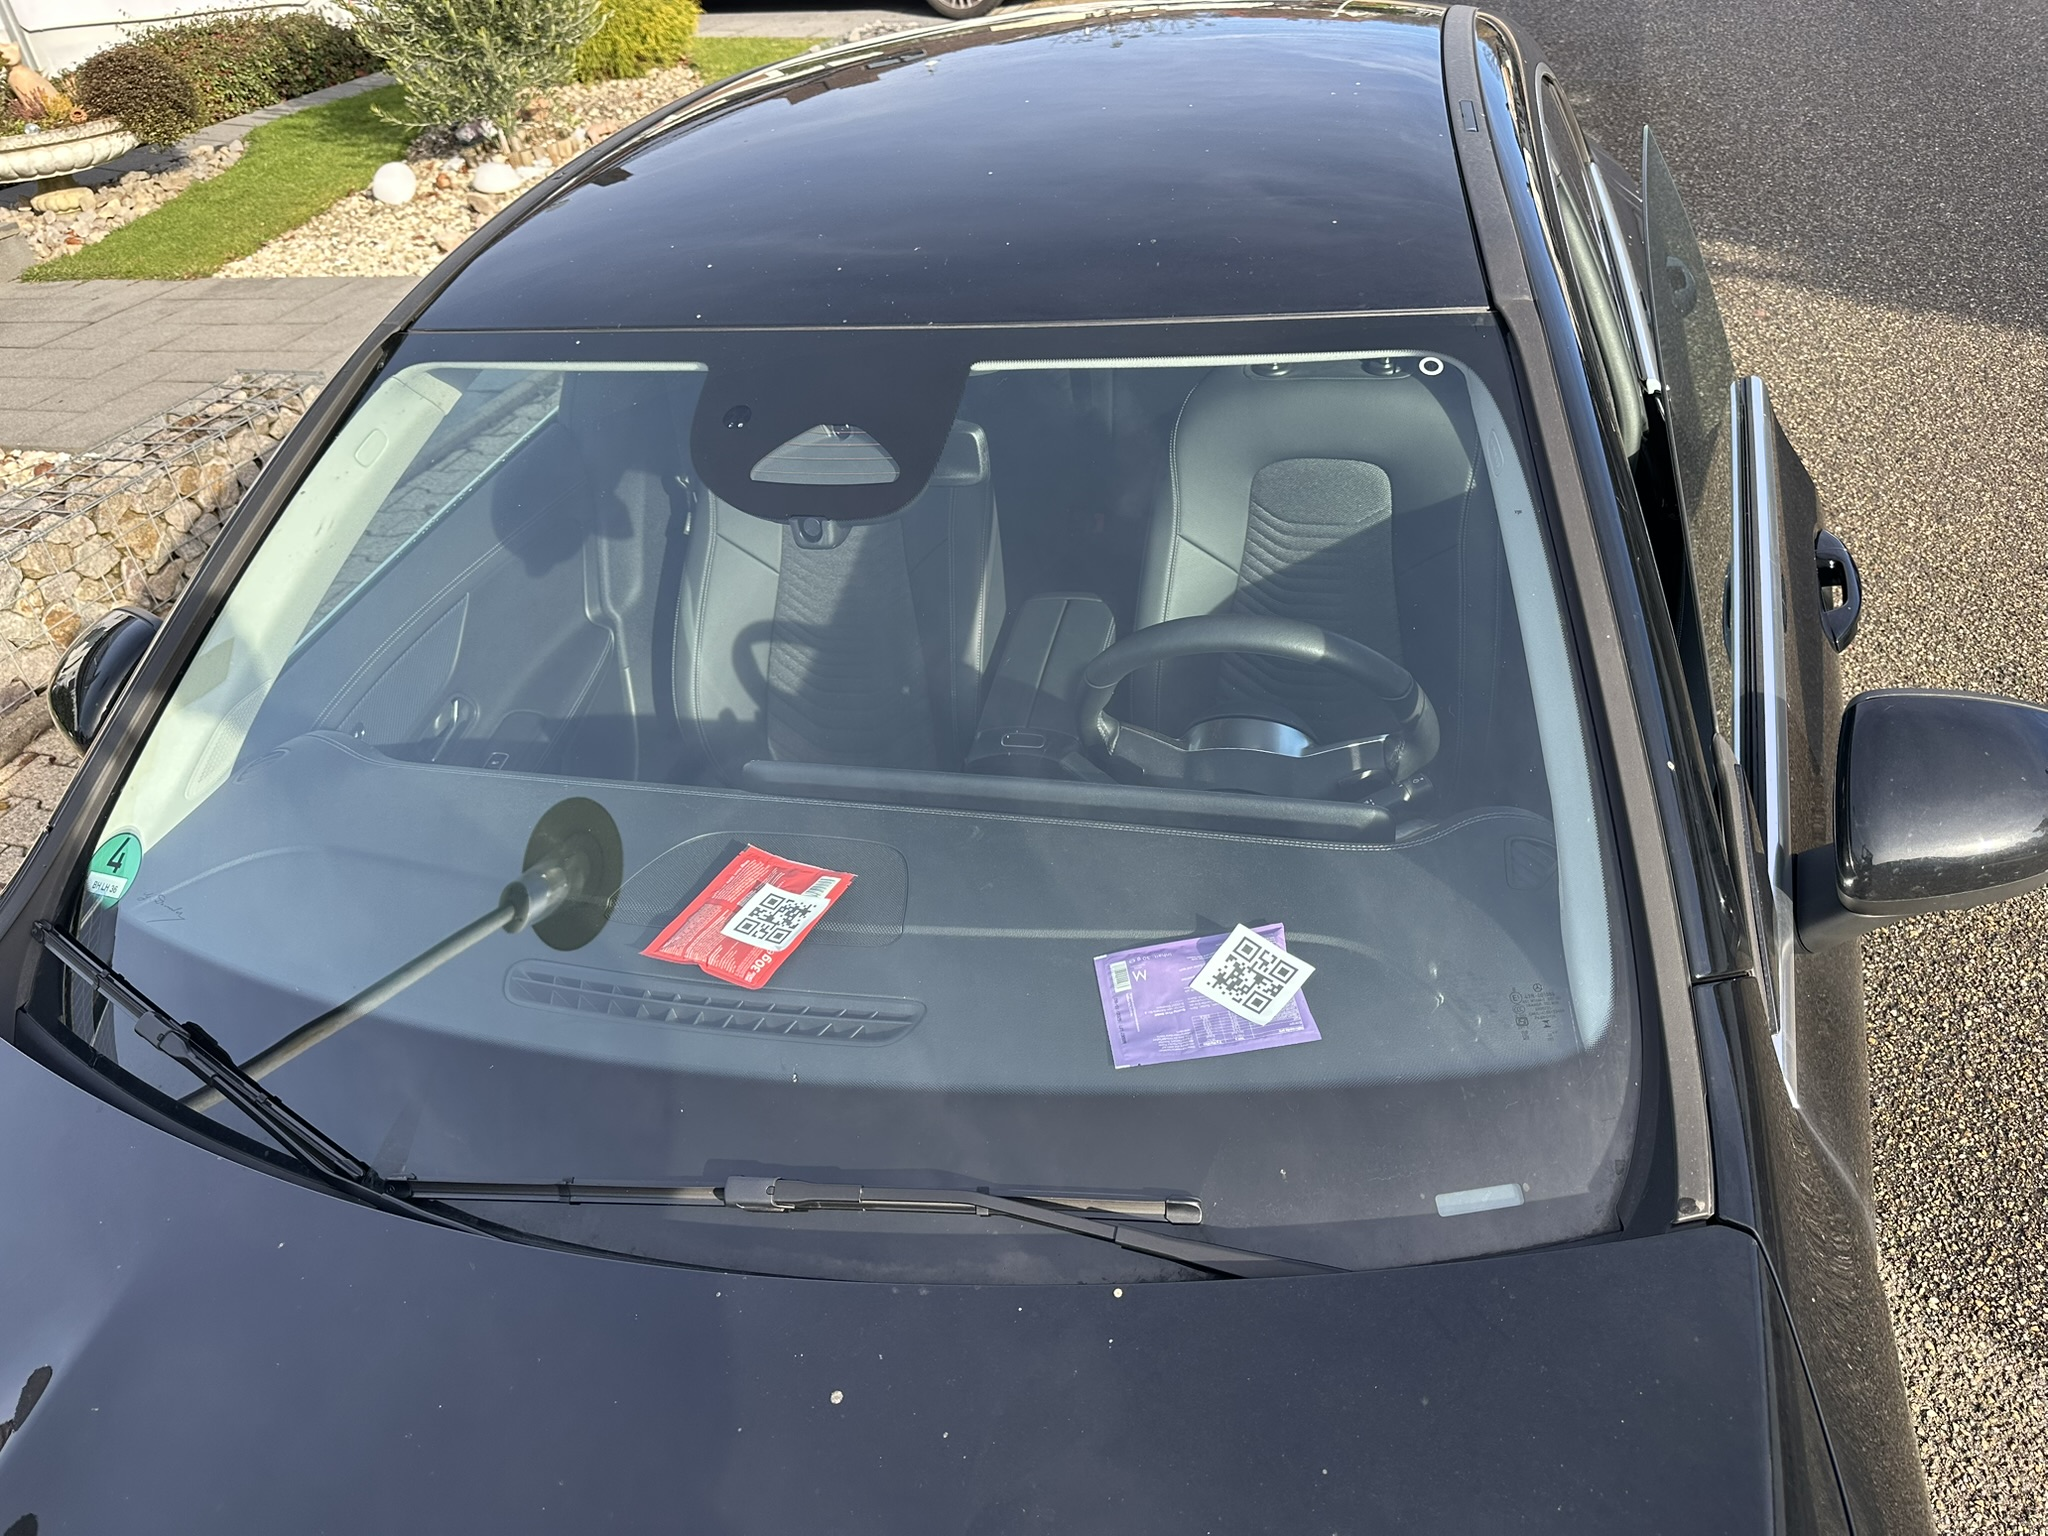
\includegraphics[width=0.8\textwidth]{Originalbild.png}
    \caption{Beispiel zur Analyse}
    \label{fig:patch_example}
\end{figure}


\subsection{Vorverarbeitung: Multi-Scale Sliding Window}

Um der Herausforderung variabler Distanzen von bis zu \SI{3}{\meter} zu begegnen, wird ein patch-basierter Ansatz gewählt. Anstatt das Bild pauschal zu skalieren und dabei kritische Details zu verlieren, gleitet ein virtuelles Fenster über die Aufnahme. Durch die Verwendung verschiedener Skalierungsfaktoren wird eine Skaleninvarianz erreicht, die es ermöglicht, QR-Codes unabhängig von ihrer physischen Entfernung zur Kamera in einer optimalen Auflösung zu erfassen.

\subsubsection{Implementierung und Konfiguration}

Die technische Umsetzung erfolgt über eine zentrale Konfigurationsstruktur, welche die Dynamik des Fensters steuert. Der folgende Code-Ausschnitt zeigt die im Projekt verwendete Konfiguration:

\begin{lstlisting}[language=Python, caption={Konfiguration der Sliding Window Parameter}]
@dataclass
class MultiScaleConfig:
    patch_size: int = 256
    scale_divisors: list = [1.5, 2.0, 3.0, 4.0, 6.0, 8.0]
    overlap: float = 0.5 
    use_relative_min_size: bool = True
    min_relative_factor: float = 0.15
    absolute_pixel_floor: int = 128
    interpolation: int = cv2.INTER_AREA
\end{lstlisting}

\subsubsection{Analyse der Einstellparameter}

Die Effizienz der Detektion hängt maßgeblich von der Justierung dieser Parameter ab:

\begin{table}[H]
    \centering
    \caption{Erläuterung der Sliding-Window-Parameter}
    \begin{tabular}{l p{9cm}}
        \toprule
        \textbf{Parameter} & \textbf{Funktion und Auswirkung} \\
        \midrule
        \texttt{patch\_size} & Definiert die quadratische Zielgröße (256 Pixel), auf die jeder Ausschnitt skaliert wird. \\
        \texttt{scale\_divisors} & Bestimmt die Skalierungsstufen. Kleine Divisoren finden nahe Objekte, große Faktoren isolieren weit entfernte QR-Codes. \\
        \texttt{overlap} & Regelt die Überlappung benachbarter Fenster (\SI{50}{\percent}). Dies stellt sicher, dass Objekte an den Schnittkanten zweier Fenster lückenlos erfasst werden. \\
        \texttt{min\_relative\_factor} & Definiert eine minimale Fenstergröße relativ zur Bildkante, um bei sehr hohen Auflösungen die Erzeugung informationsloser Patches zu verhindern. \\
        \texttt{interpolation} & Nutzt \texttt{cv2.INTER\_AREA}, was beim Verkleinern von Bildbereichen die beste Bildqualität liefert. \\
        \bottomrule
    \end{tabular}
\end{table}

\begin{figure}[H]
    \centering
    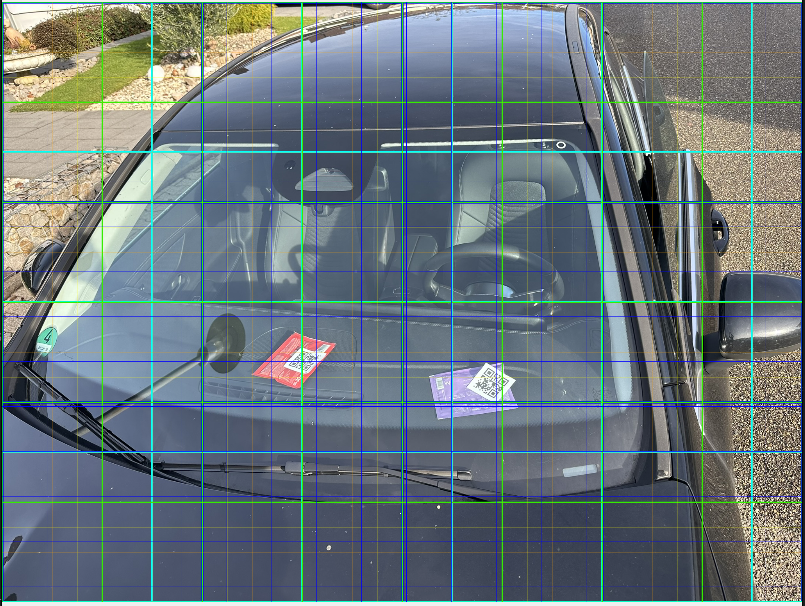
\includegraphics[width=0.8\textwidth]{SlidingWindows.png}
    \caption{Visualisierung des Sliding-Window-Rasters über verschiedene Skalierungsstufen hinweg.}
    \label{fig:sliding_window_grid}
\end{figure}

Die farbigen Gitterlinien in Abbildung \ref{fig:sliding_window_grid} markieren die Grenzen der extrahierten \textbf{Patches}. Jede Farbe entspricht dabei einer spezifischen Fenstergröße, resultierend aus den konfigurierten Skalierungs-Divisoren:

\begin{itemize}
    \item \textbf{Blau:} Divisoren \num{1,5} und \num{8,0} (größte und kleinste \textbf{Bildausschnitte}).
    \item \textbf{Cyan:} Divisor \num{2,0}.
    \item \textbf{Grün:} Divisor \num{3,0}.
    \item \textbf{Gelb:} Divisor \num{4,0}.
    \item \textbf{Orange:} Divisor \num{6,0}.
\end{itemize}

Durch die Überlappung (\textit{Overlap}) von \SI{50}{\percent} entsteht ein feinmaschiges Gittermuster. Dieses stellt sicher, dass relevante Objekte unabhängig von ihrer Position im \textbf{Gesamtbild} vollständig erfasst werden, da sie in mindestens einem der überlappenden \textbf{Patches} zentral abgebildet werden.

\subsubsection{Normalisierung und mathematische Zusammenhänge}

Nach der Extraktion wird jeder Patch normalisiert. In diesem Kontext bedeutet \textbf{Normalisierung}, dass die ganzzahligen Pixelwerte (0 bis 255) in eine Fließkommadarstellung (typischerweise im Bereich von 0.0 bis 1.0) transformiert werden. Dieser Schritt ist essenziell für die numerische Stabilität des neuronalen Netzes, da er sicherstellt, dass die Eingangsdaten eine einheitliche Skalierung aufweisen und das Training bzw. die Inferenz nicht durch hohe Absolutwerte verzerrt wird.

Die Schrittweite (\textit{Stride}), mit der das Fenster wandert, berechnet sich dynamisch aus der Fenstergröße ($win\_size$) und dem \texttt{overlap}:

$$ stride = max(1, int(win\_size \cdot (1 - overlap))) $$

Dieses Verfahren ermöglicht eine vollständige Auflösungsunabhängigkeit. Ob ein Full-HD oder ein 4K-Bild verarbeitet wird, beeinflusst lediglich die Anzahl der Patches, nicht aber deren relative Detailtiefe.

\begin{figure}[H]
    \centering
    % Drei Bilder bei 0.3\textwidth lassen Platz für Lücken dazwischen
    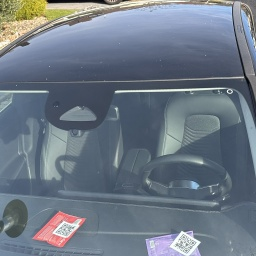
\includegraphics[width=0.3\textwidth]{Beispielpatch_0.jpg}
    \hfill
    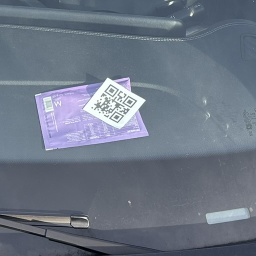
\includegraphics[width=0.3\textwidth]{Beispielpatch_2.jpg}
    \hfill
    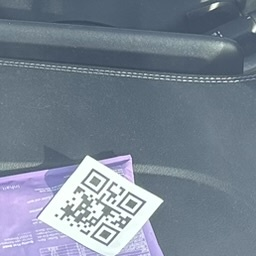
\includegraphics[width=0.3\textwidth]{Beispielpatch_4.jpg}
    
    \caption{Drei unterschiedliche SlidingWindow-Größen bei der gleichen Bildregion}
    \label{fig:patch_overlap}
\end{figure}

\subsection{Modelldurchlauf}

Nachdem das Bild durch das Sliding-Window-Verfahren in eine Menge normalisierter Patches zerlegt wurde, erfolgt der eigentliche Modelldurchlauf. In dieser Phase fungiert das neuronale Netz als Klassifikator, um für jeden einzelnen Bildausschnitt die Wahrscheinlichkeit zu bestimmen, mit der dieser einen QR-Code enthält.

\subsubsection{Datenvorbereitung und Farbraumanpassung}

Ein kritischer Schritt vor der eigentlichen Inferenz ist die Anpassung der Bilddaten an das gewählte Modell. Da die Inferenz-Pipeline flexibel verschiedene Architekturen unterstützt, findet eine einheitliche Vorverarbeitung für alle Modelltypen statt:
\begin{itemize}
    \item \textbf{Kanal-Formatierung:} Alle Patches werden direkt in Graustufen geladen und um eine Kanaldimension erweitert, um dem erwarteten Eingangsformat des jeweiligen Netzes zu entsprechen.
    \item \textbf{Modell-Kompatibilität:} Bei den Transfer-Learning-Modellen ermöglicht ein Grayscale-Adapter die Verarbeitung einkanaliger Daten, wodurch eine Farbraum-Konvertierung nicht notwendig ist. 
\end{itemize}
Zusätzlich werden alle Bilddaten in den Datentyp \texttt{float32} konvertiert, um eine präzise Verarbeitung durch die Gewichte des neuronalen Netzes zu gewährleisten.
\subsubsection{Batch-Verarbeitung und VRAM-Management}

Um die Inferenzzeit bei der hohen Anzahl an extrahierten Patches (oft mehrere hundert pro Bild) zu minimieren, werden diese gesammelt in Batches verarbeitet. Dies erlaubt es der Grafikhardware, die Berechnungen durch massive Parallelisierung zu beschleunigen. 

Da die Anzahl der Patches bei hochauflösenden 4K-Aufnahmen den verfügbaren Grafikspeicher (VRAM) überschreiten kann, wurde ein robustes Fehlermanagement implementiert. Das System nutzt eine iterative Batch-Größen-Anpassung: Sollte ein \texttt{ResourceExhaustedError} auftreten, wird die Batch-Größe halbiert und der Arbeitsspeicher bereinigt, bis die Inferenz stabil durchgeführt werden kann. Nach jedem Bilddurchlauf wird zudem die Keras-Session zurückgesetzt, um Speicherlecks langfristig zu vermeiden.

\begin{lstlisting}[language=Python, caption={Logik des Modelldurchlaufs mit dynamischem VRAM-Schutz}]
# Vorhersage mit dynamischer Batch-Groesse
preds = None
current_bs = cfg.start_batch_size
while current_bs >= 1:
    try:
        preds = model.predict(input_batch, batch_size=current_bs, verbose=0)
        break 
    except tf.errors.ResourceExhaustedError:
        print(f"VRAM Limit erreicht, reduziere Batch auf {current_bs // 2}")
        current_bs //= 2
        gc.collect()
\end{lstlisting}

\subsection{Heatmap Erstellung}

Das Ergebnis des Modelldurchlaufs ist eine Liste von Wahrscheinlichkeiten für alle extrahierten Patches. Da sich die Sliding Windows aufgrund des gewählten Overlaps und der verschiedenen Skalierungsstufen vielfach überschneiden, liegen für fast jede Bildregion mehrere Vorhersagen vor. Die Heatmap dient dazu, diese verstreuten Informationen zu fusionieren und eine räumliche Wahrscheinlichkeitsverteilung über das gesamte Originalbild zu legen.

\subsubsection{Das Voting-Prinzip der Wahrscheinlichkeits-Akkumulation}

Die Erstellung der Heatmap folgt einem akkumulativen \glqq Voting-Verfahren\grqq . Hierzu wird zunächst eine Matrix in der exakten Dimension des Originalbildes mit Nullwerten initialisiert. Das System iteriert anschließend durch alle Patches und deren zugehörige Modellvorhersagen.

Ein Patch gibt nur dann eine \glqq Stimme\grqq\ ab, wenn seine Konfidenz den Schwellenwert \texttt{min\_vote\_prob} überschreitet. Ist dies der Fall, wird die gesamte Wahrscheinlichkeit auf den entsprechenden Bereich der Heatmap-Matrix addiert. Pixel, die Teil eines QR-Codes sind, befinden sich durch den Multi-Scale-Ansatz in zahlreichen positiven Patches unterschiedlicher Größe. Durch die Addition dieser Werte entstehen in der Matrix lokale Maxima, sogenannte Hotspots. Zufällige Fehlklassifikationen (False Positives), die meist nur in einer einzigen Skalierung oder an einer spezifischen Position auftreten, erreichen dadurch niemals die notwendige kumulierte Summe, um als Detektion gewertet zu werden.

\begin{figure}[H]
    \centering
    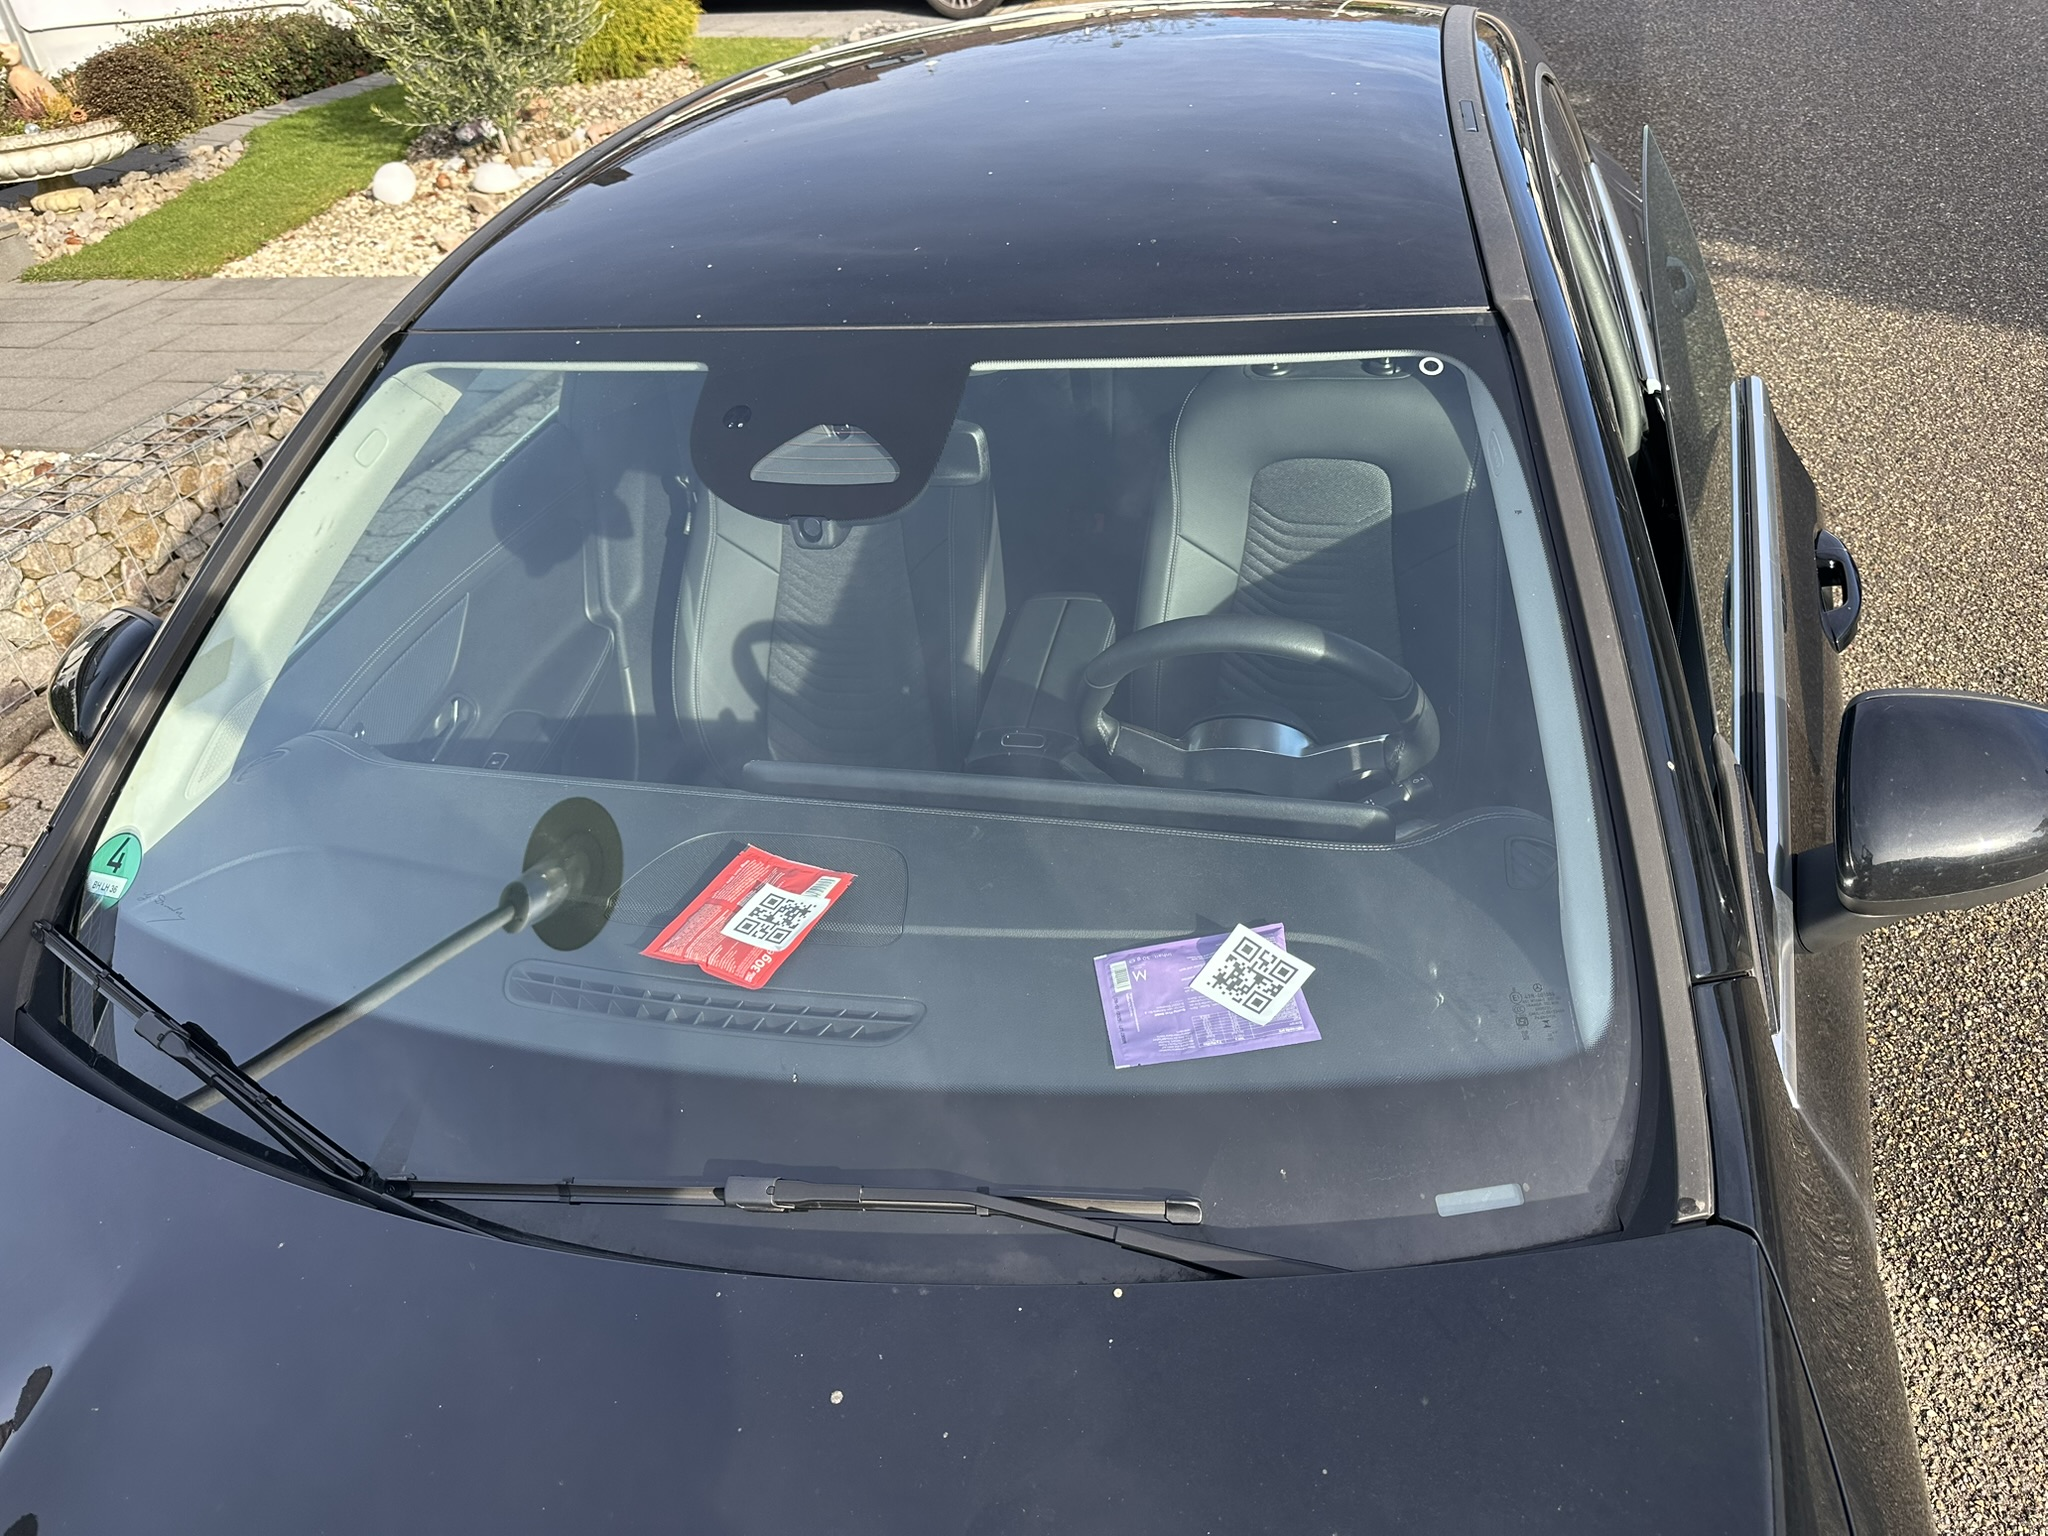
\includegraphics[width=0.47\textwidth]{Originalbild.png}
    \hfill
    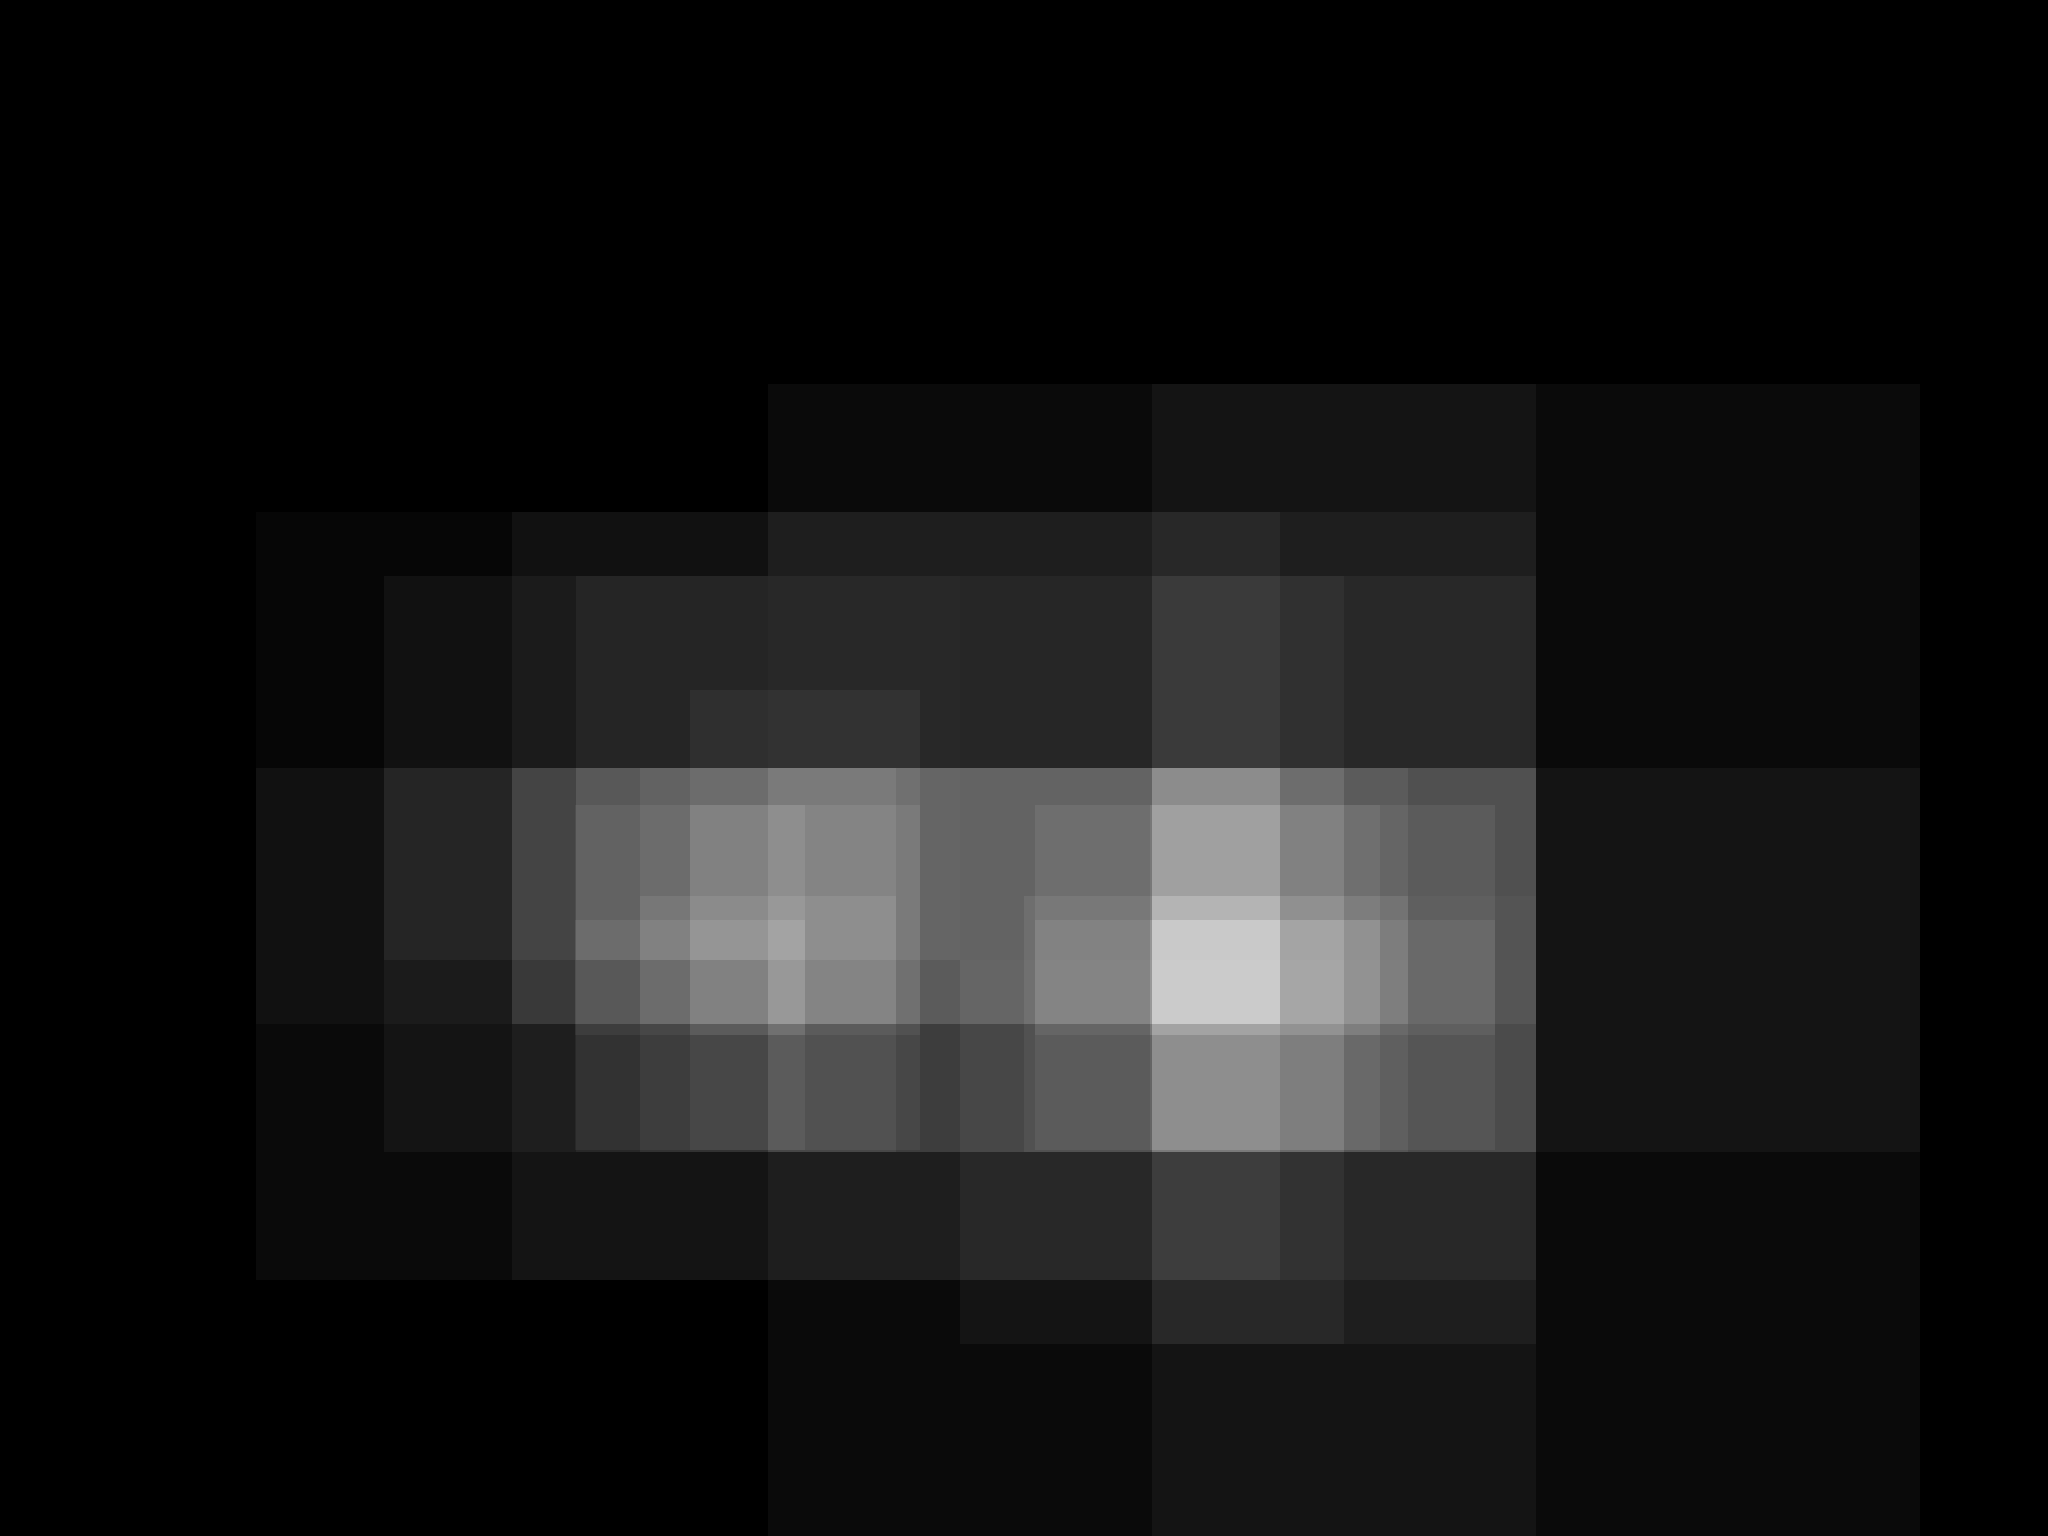
\includegraphics[width=0.47\textwidth]{Heatmap.png}
    \caption{Visualisierung des Prozesses: Vom Originalbild (links) zur akkumulierten Wahrscheinlichkeitsverteilung (rechts).}
    \label{fig:heatmap_process}
\end{figure}

\subsubsection{Konfigurationsparameter und Visualisierung}

Die Sensitivität und Präzision der Detektion lässt sich über drei zentrale Parameter steuern, die im Jupyter Notebook definiert sind:

\begin{table}[H]
    \centering
    \caption{Zentrale Parameter der Heatmap-Logik}
    \begin{tabular}{l p{9cm}}
        \toprule
        \textbf{Parameter} & \textbf{Bedeutung und Funktion} \\
        \midrule
        \texttt{min\_vote\_prob} & Ein Schwellenwert (z. B. 0.3), der als Filter fungiert. Nur Patches, die sich das Modell \glqq sicher genug\grqq\ ist, fließen in die Heatmap ein. \\
        \texttt{vote\_threshold} & Das finale Entscheidungskriterium (z. B. 5.0). Erst wenn die Summe der Wahrscheinlichkeiten an einer Stelle diesen Wert überschreitet, wird dort ein Objekt vermutet. \\
        \texttt{fixed\_vis\_max} & Dieser Parameter definiert den Endpunkt der Werteskala (z. B. 25.0) für die grafische Darstellung. Er legt fest, ab welcher Akkumulationsdichte ein Pixel in der Visualisierung als \glqq maximal heiß\grqq\ (weiß bzw. rot) dargestellt wird. \\
        \bottomrule
    \end{tabular}
\end{table}

\subsubsection{Visualisierung und Normierung (\texttt{fixed\_vis\_max})}

Da die aufsummierten Wahrscheinlichkeiten in der Heatmap-Matrix beliebige Werte annehmen können (z.\,B. eine Summe von 15,4), müssen diese für die Anzeige am Monitor in ein sichtbares Bild übersetzt werden. Ein digitaler Pixel kann Helligkeitswerte von 0 (Schwarz/Blau) bis 255 (Wei\ss/Rot) annehmen.

\begin{figure}[H]
    \centering
    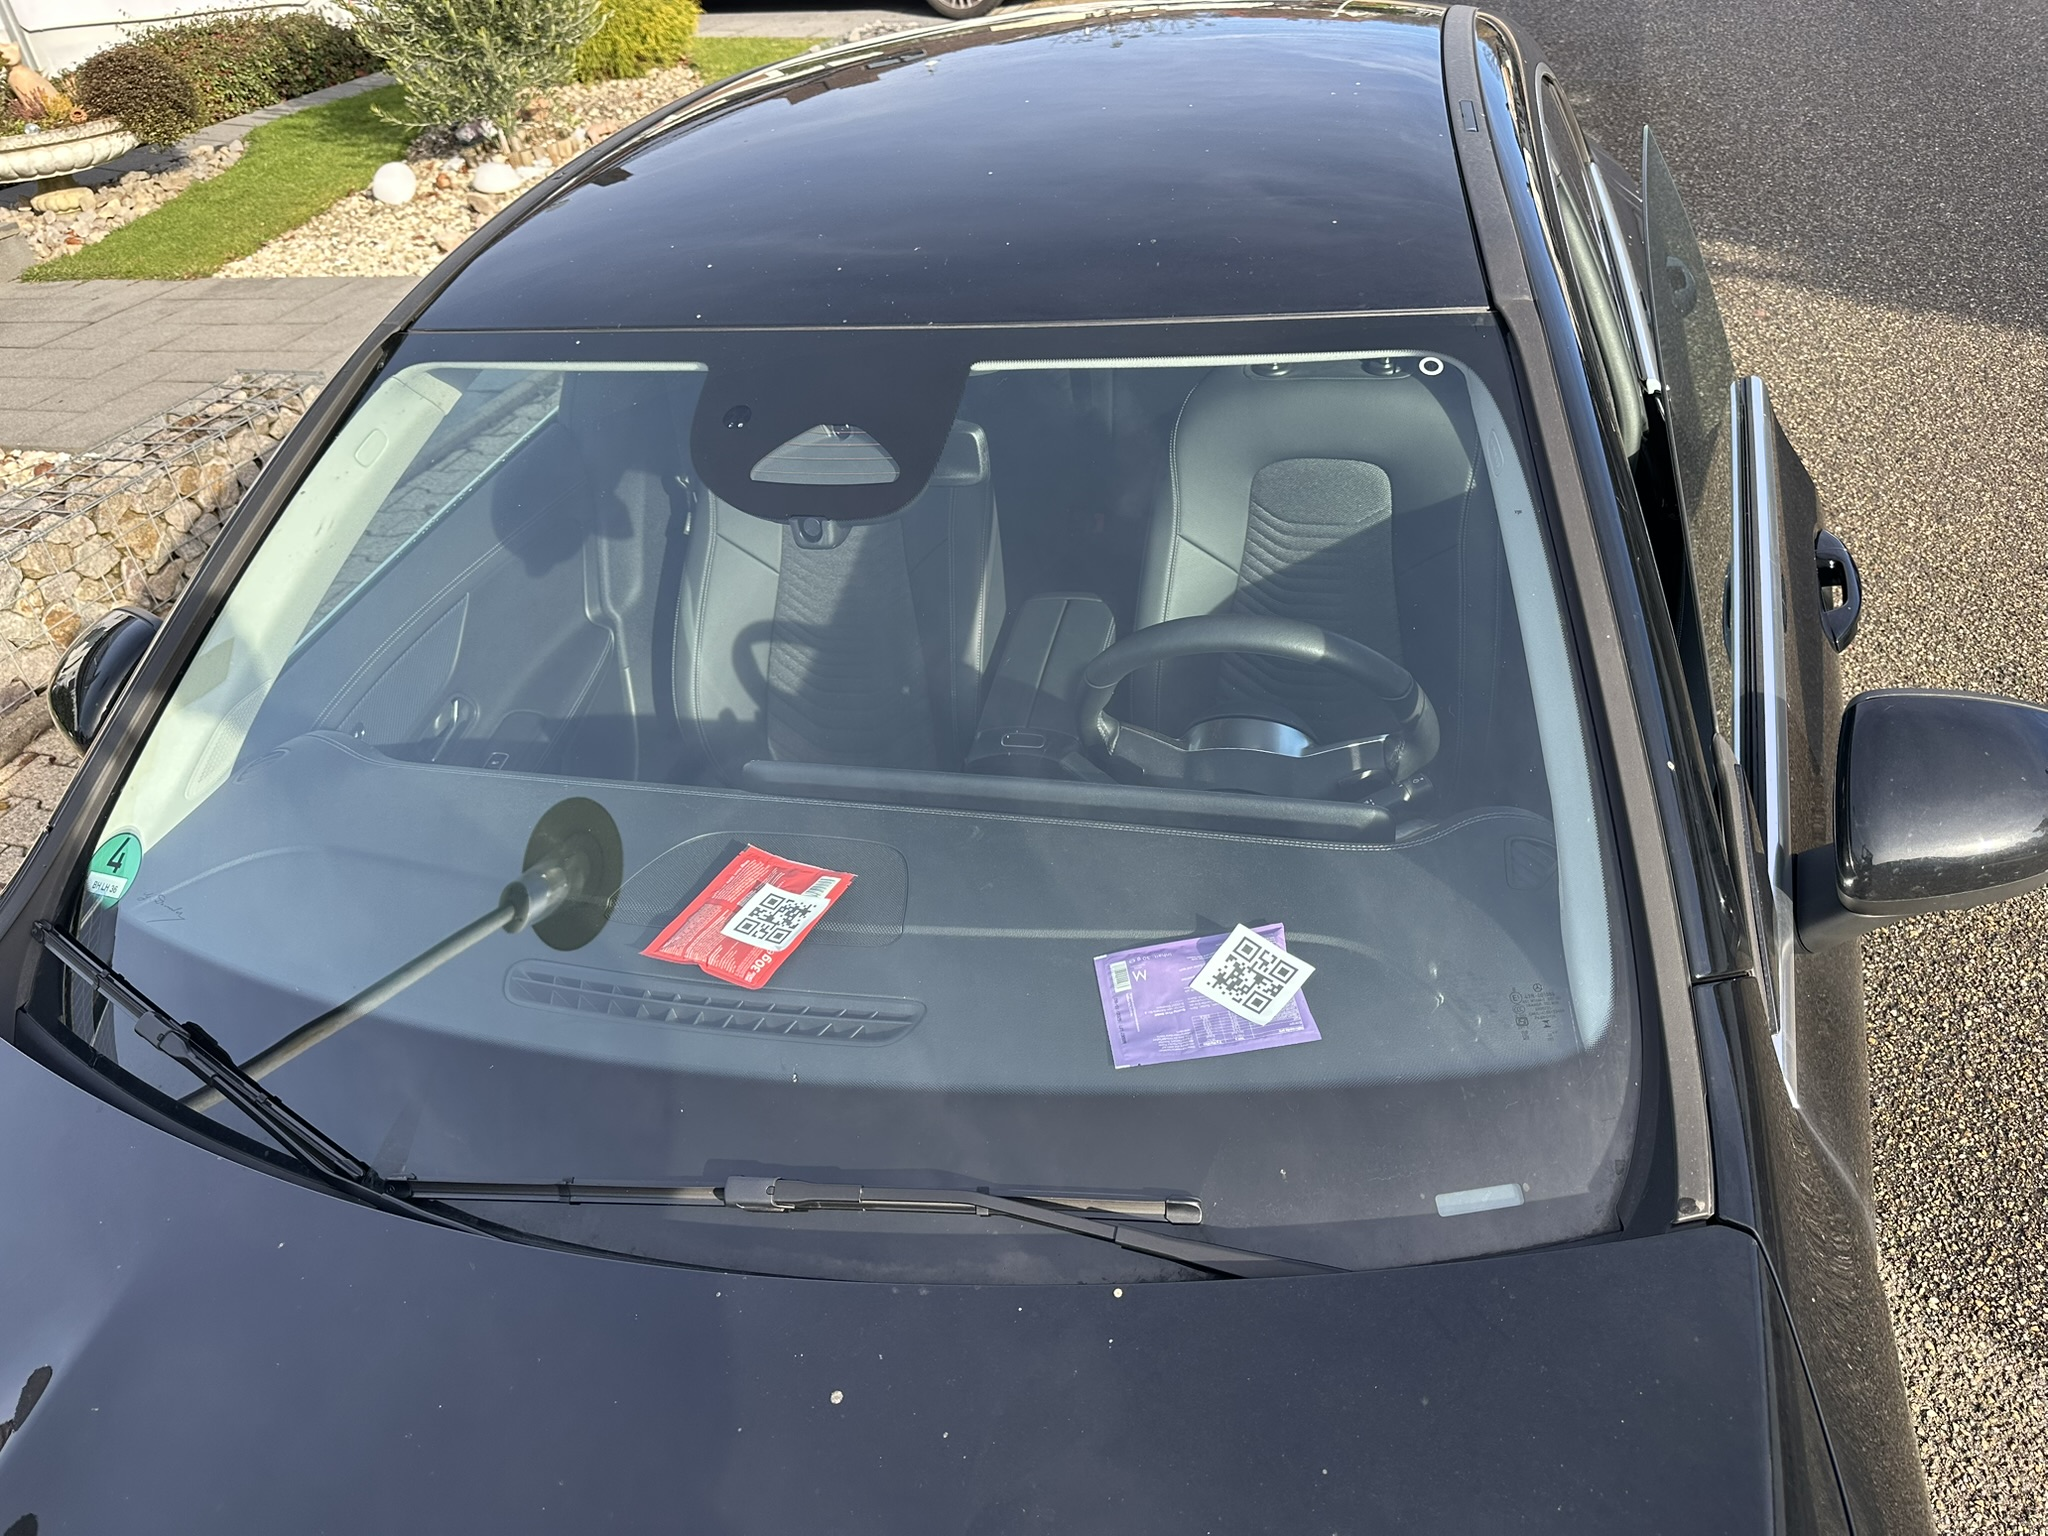
\includegraphics[width=0.47\textwidth]{Originalbild.png}
    \hfill
    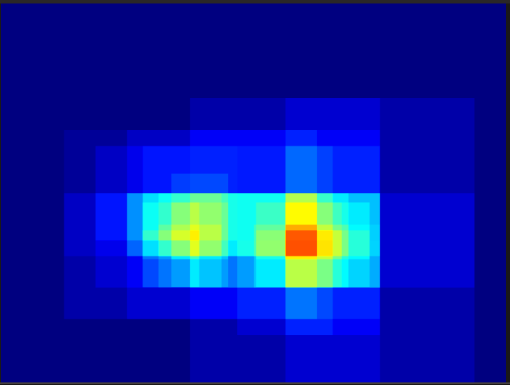
\includegraphics[width=0.47\textwidth]{Heatmap_bunt.png}
    \caption{Finale normierte Heatmap: Die roten Bereiche markieren die Zentren der detektierten QR-Codes mit höchster Konfidenz.}
    \label{fig:final_heatmap_example}
\end{figure}

Hierbei kommt der Parameter \texttt{fixed\_vis\_max} zum Einsatz. Er fungiert als \glqq Sättigungsgrenze\grqq\ bzw. als Messlatte für die maximale Helligkeit. Er definiert, ab welcher kumulierten Wahrscheinlichkeit ein Bereich im Bild als wei\ss\ / rot (maximal sicher) dargestellt werden soll. Die Umrechnung erfolgt nach der Formel:

$$\text{Pixelhelligkeit} = \min\left( \frac{\text{Akkumulierte Summe}}{\text{fixed\_vis\_max}} \cdot 255,\, 255 \right)$$

Durch diese Normierung werden die mathematischen Hotspots in eine für den Menschen interpretierbare Form übersetzt. Bereiche mit hoher Übereinstimmung erscheinen hell leuchtend, während unsichere Bereiche oder vereinzelte Fehlklassifikationen dunkel bleiben. Dies ermöglicht eine intuitive Beurteilung, wie sicher sich das System bei der Lokalisierung des QR-Codes ist.

\begin{figure}[H]
    \centering
    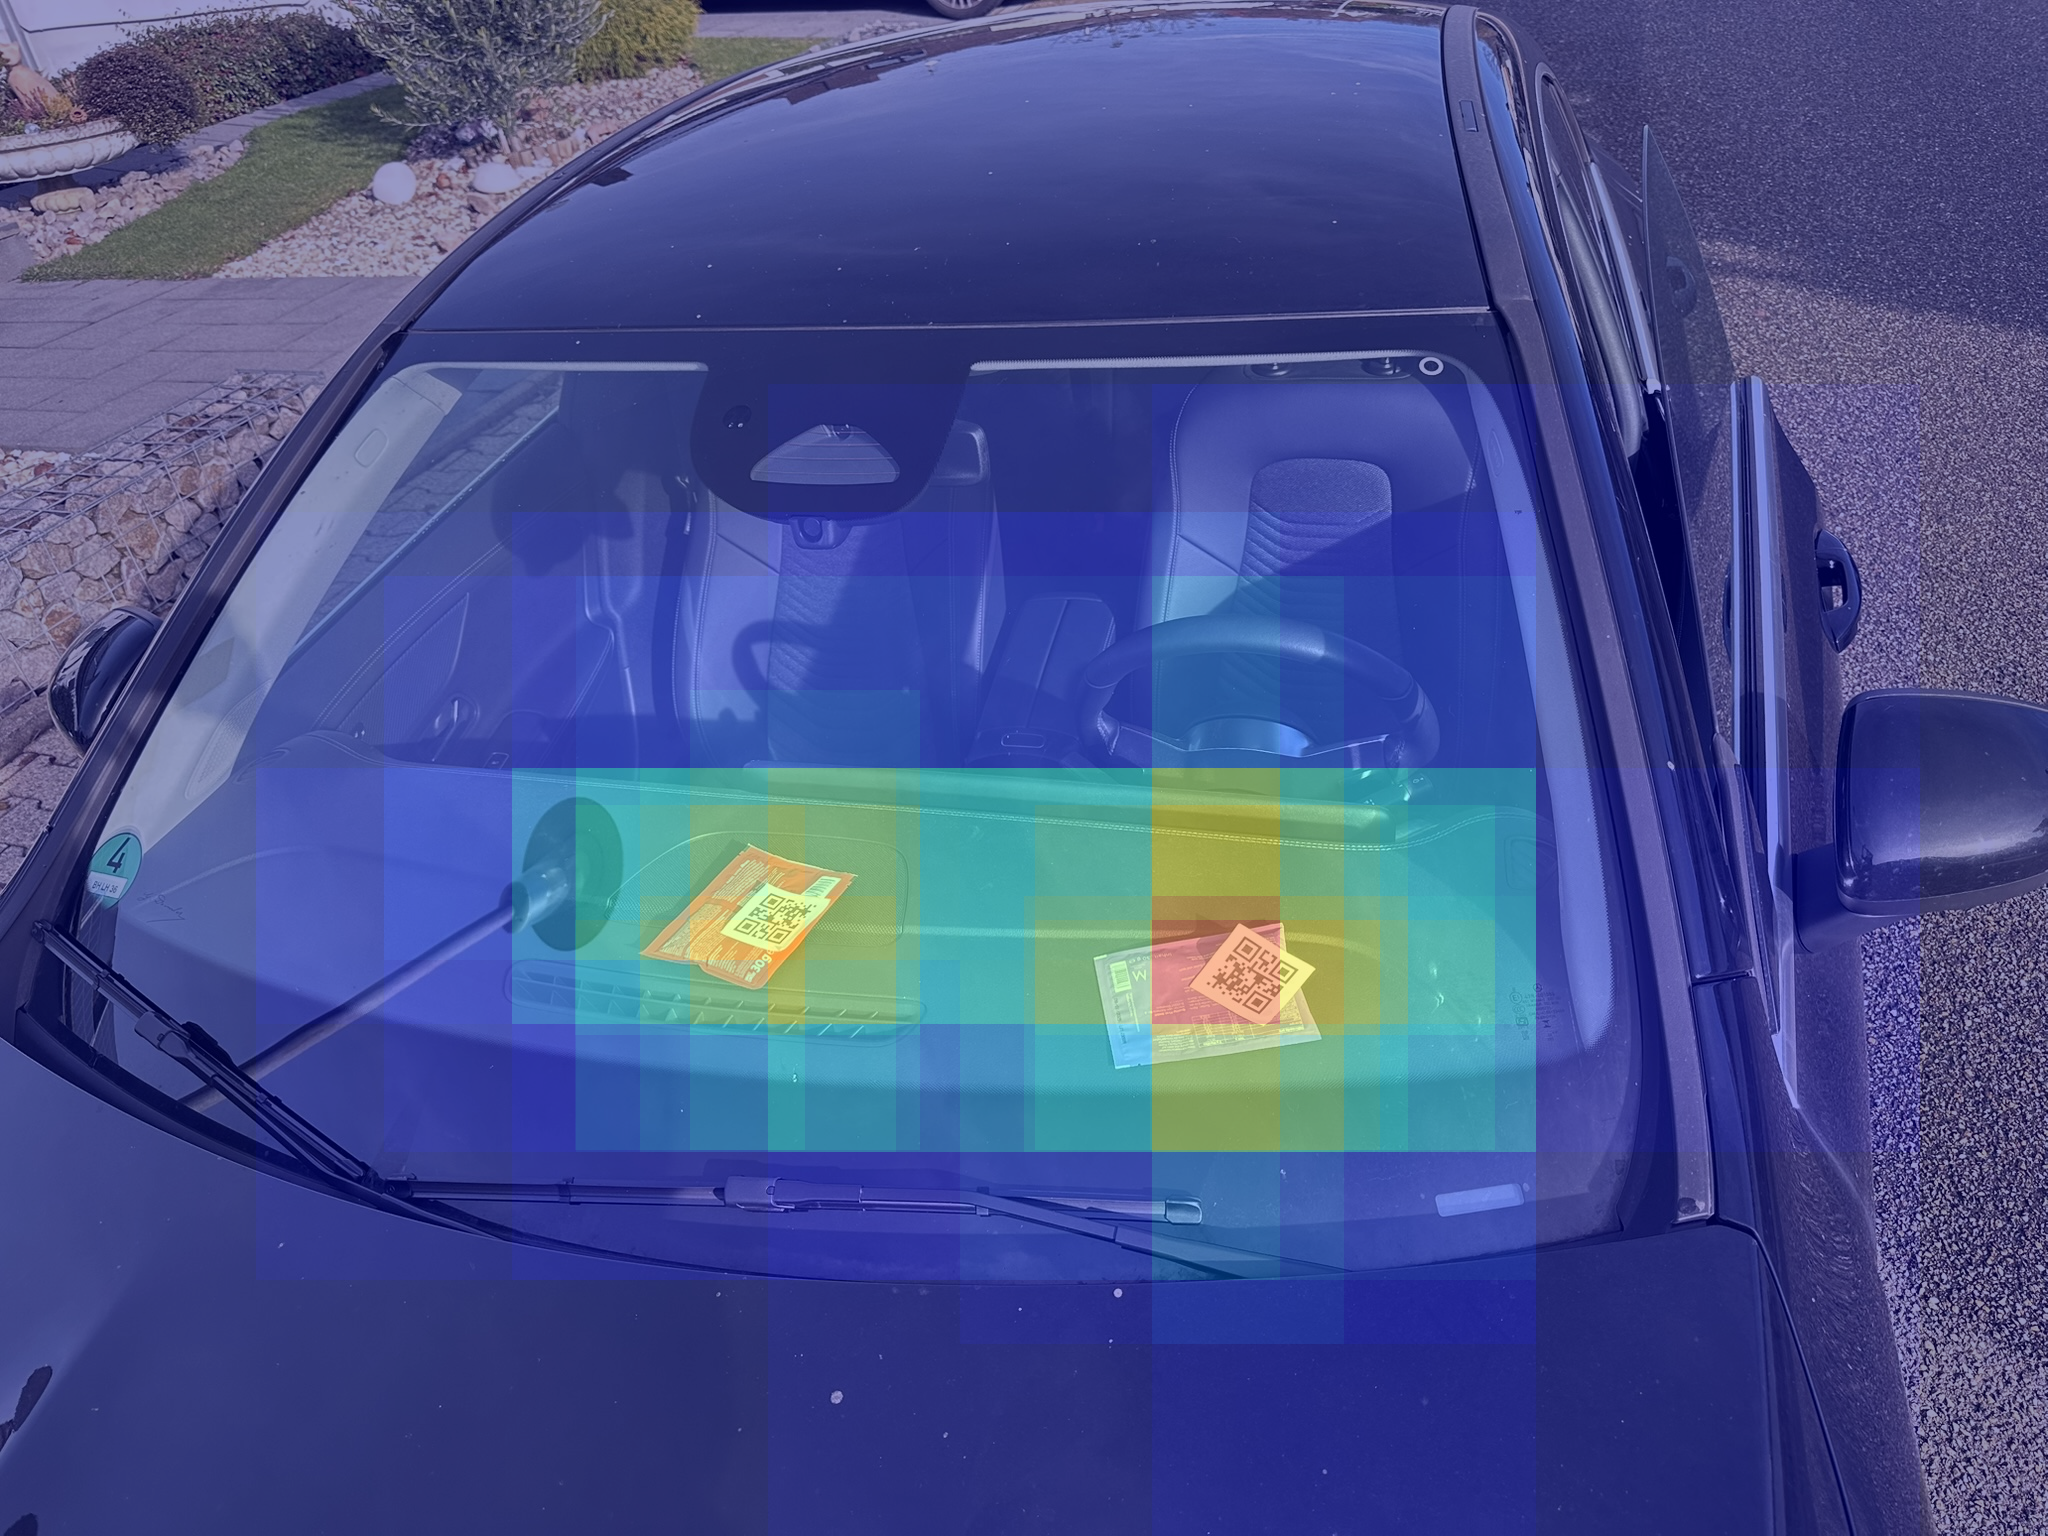
\includegraphics[width=0.5\textwidth]{Heatmap_auf_Orginalbild.png}
    \hfill
    \caption{Überlagerung der Heatmap auf das Originalbild}
    \label{fig:heatmap_x_originpicture_example}
\end{figure}

\subsection{Finale Entscheidung und Lokalisierung}

Nach der Erstellung der Heatmap muss das System eine binäre Entscheidung treffen, ob ein QR-Code im Bild vorhanden ist. % 
In diesem abschließenden Schritt der Inferenz-Pipeline werden die kontinuierlichen Wahrscheinlichkeitswerte der Heatmap in präzise Koordinaten umgewandelt. % 

\subsubsection{Binarisierung: Trennung von Signal und Rauschen}

Die Heatmap lässt sich grafisch als eine Landschaft mit unterschiedlich hohen Erhebungen beschreiben, wobei die Höhe der \glqq Berge\grqq\ die Wahrscheinlichkeit für einen QR-Code repräsentiert. % 
Um daraus eine eindeutige Entscheidung abzuleiten, wird diese Landkarte in ein klares Schwarz-Wei\ss-Bild (Binärmaske) transformiert. % 

Hierbei fungiert der \texttt{vote\_threshold} als eine Art \glqq Türsteher\grqq: Nur Bereiche, die in der Summe genug Stimmen (z.\,B. einen kumulierten Wert von 5,0) gesammelt haben, werden als wei\ss\ markiert. % 
Alle Bereiche unterhalb dieses Wertes werden auf Null gesetzt und somit als Hintergrund (schwarz) eingestuft. % 
Dieser Schritt ist entscheidend für die Stabilität des Systems, da vereinzelte Fehlklassifikationen, die nur in einem einzelnen Patch auftraten, niemals die notwendige Stimmenanzahl erreichen und somit rigoros herausgefiltert werden. % 

\subsubsection{Lokalisierung und geometrische Plausibilitätsprüfung}

Nach der Bereinigung der Heatmap liegen oft isolierte wei\ss e Flächen vor, die potenzielle Standorte von QR-Codes markieren. % 
Um diese Flächen als eigenständige Objekte greifbar zu machen, wird ein Algorithmus zur Konturfindung (\texttt{cv2.findContours}) eingesetzt, der zusammenhängende Pixel-Inseln identifiziert und deren Au\ss engrenzen definiert. % 



Jede gefundene Kontur wird anschließend einer geometrischen Plausibilitätsprüfung unterzogen, um Fehlalarme durch optisches Rauschen oder feine Hintergrundmuster auszuschlie\ss en. % 
Hierzu wird mit \texttt{cv2.boundingRect} das kleinste umschlie\ss ende Rechteck für jede Insel berechnet: % 
\begin{itemize}
    \item Da ein echter QR-Code im Kamerabild immer eine gewisse Mindestgröße aufweisen muss, werden extrem kleine Konturen (unter $30 \times 30$ Pixeln) ignoriert. % 
    \item Diese Filterung stellt sicher, dass nur signifikante Merkmale zur weiteren Analyse an den Decoder übergeben werden. % 
\end{itemize}

\subsubsection{Visualisierung der Detektion}

Wurde mindestens eine valide Kontur gefunden, gilt das Bild als \glqq QR DETECTED\grqq. Zur Dokumentation und visuellen Verifikation wird die Lokalisierung im Ausgabebild hervorgehoben:
\begin{itemize}
    \item \textbf{Bounding Box:} Um das detektierte Objekt wird ein grüner Rahmen mit einer definierten Linienstärke gezeichnet.
    \item \textbf{Status-Anzeige:} Im Evaluation-Dashboard wird zusätzlich der berechnete \glqq Real Score\grqq\ (die maximale Dichte der Heatmap) sowie die finale Entscheidung ausgegeben.
\end{itemize}

\begin{figure}[H]
    \centering
    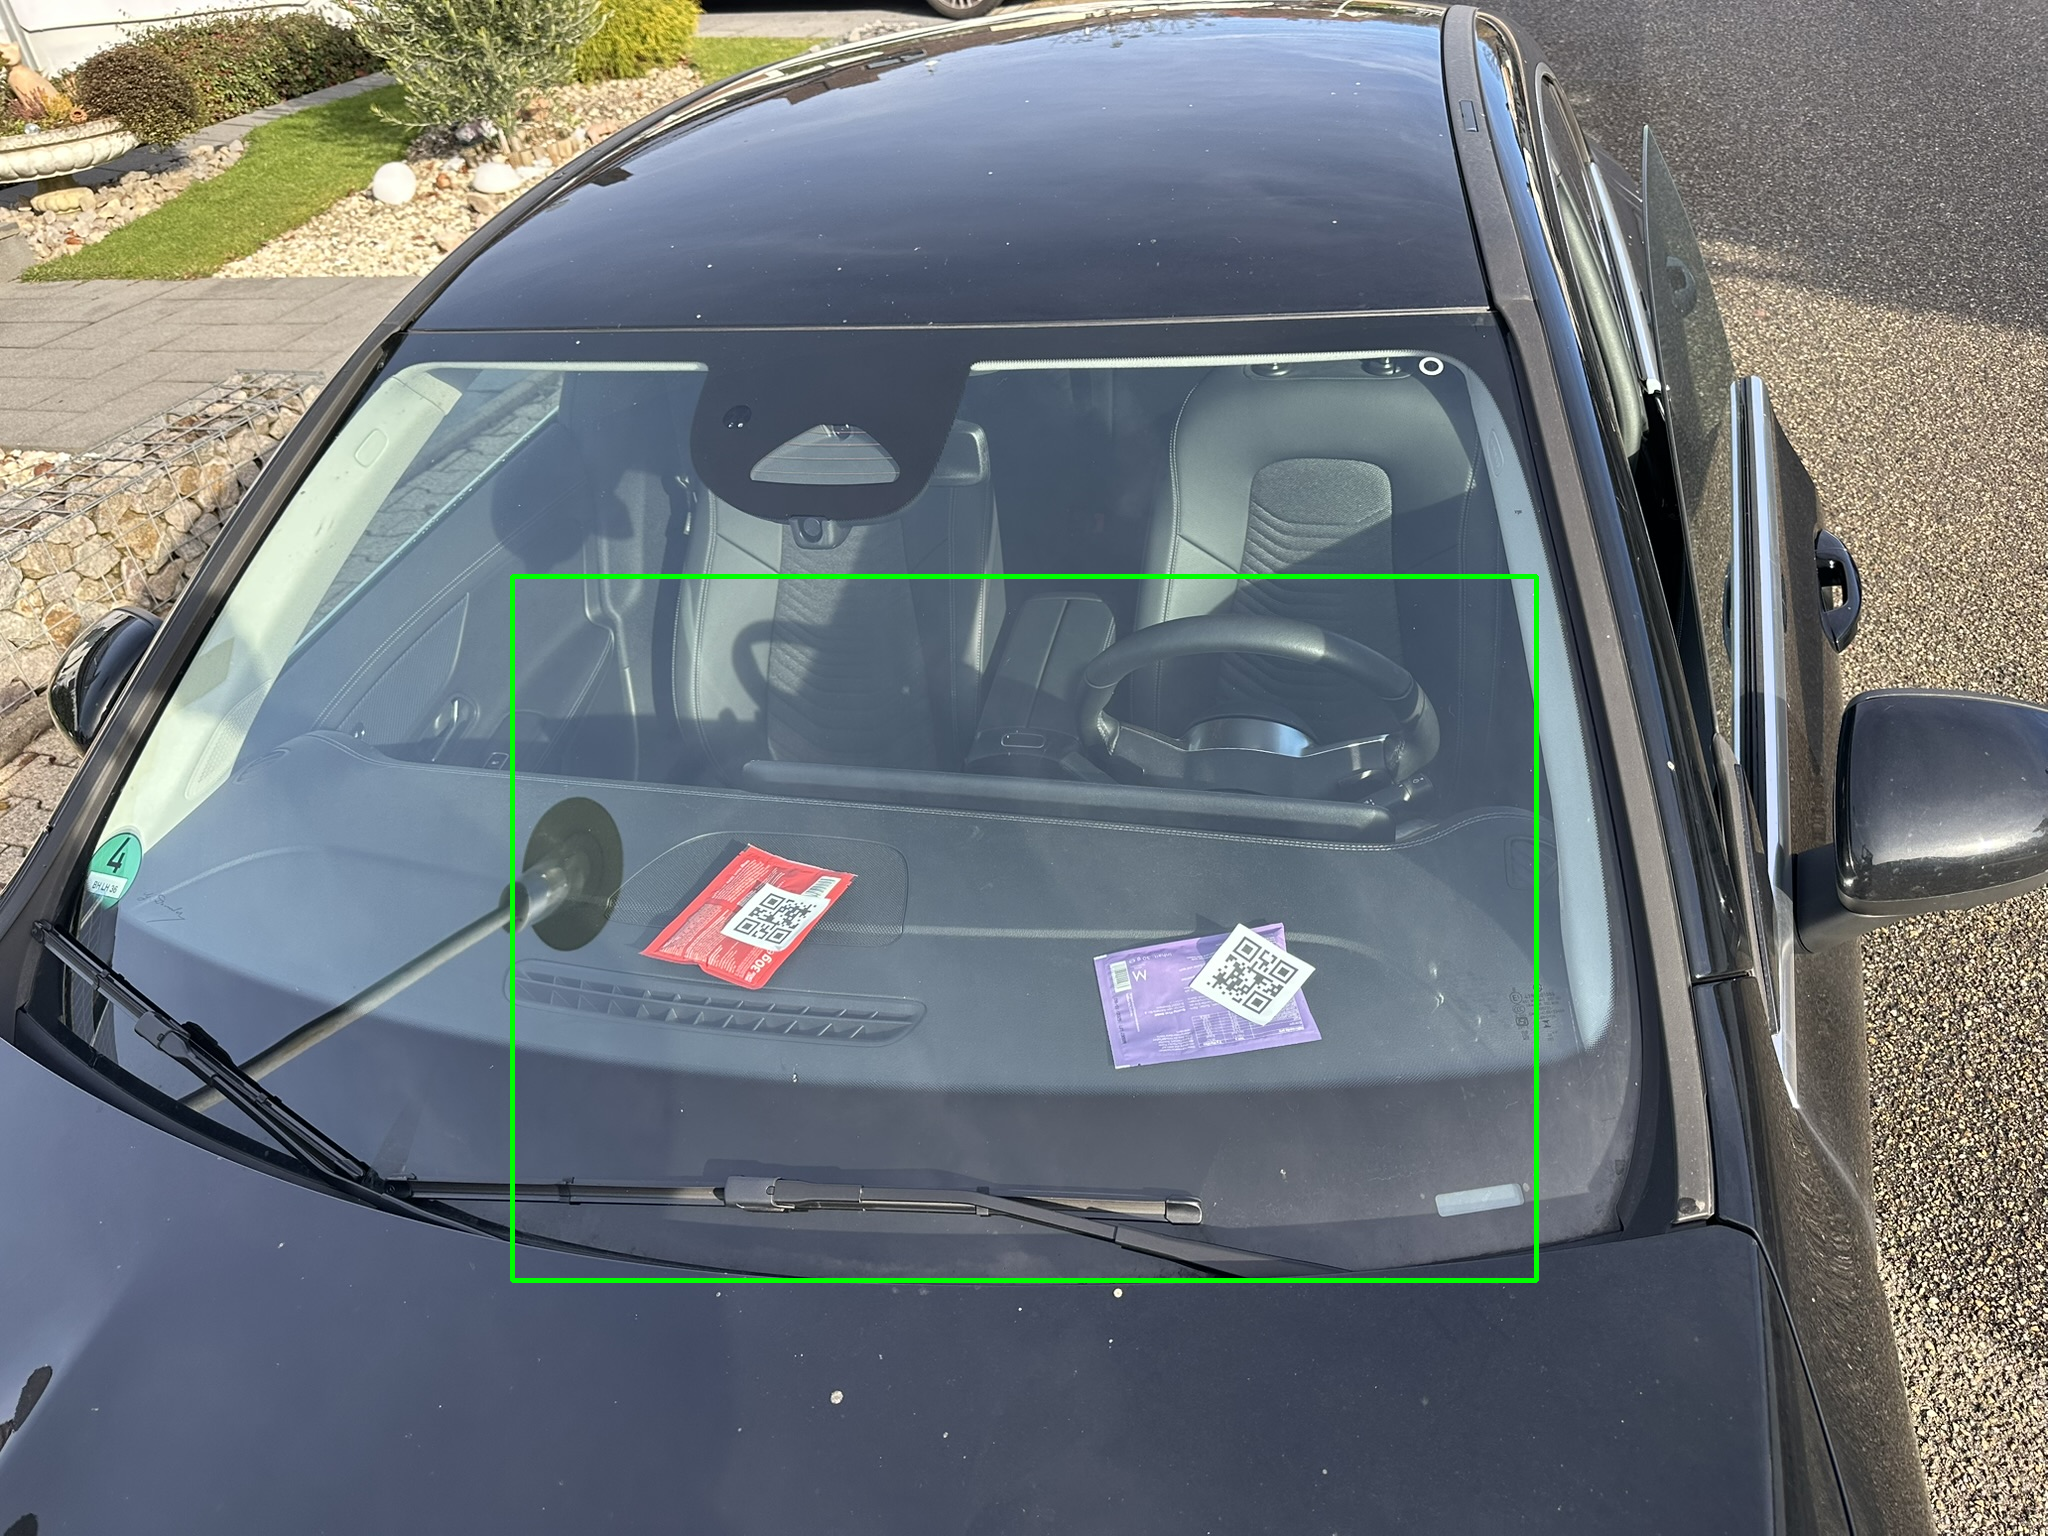
\includegraphics[width=0.8\textwidth]{ROI_Kennzeichnung.PNG}
    \caption{Finales Ergebnis der Inferenz: Der lokalisierte QR-Code wird durch eine grüne Bounding Box im Originalbild hervorgehoben.}
    \label{fig:bounding_box}
\end{figure}

Sollten keine Konturen den \texttt{vote\_threshold} und die Größenfilterung passieren, wird das Bild als \glqq NO DETECTION\grqq\ markiert. Dies stellt sicher, dass die nachgelagerte und rechenintensive Decodierung nur auf Bildbereichen ausgeführt wird, in denen mit hoher Sicherheit ein QR-Code vorliegt.

\subsubsection{Visuelle Ergebniskontrolle: Das Evaluations-Dashboard}

Das zur Ergebniskontrolle implementierte Dashboard führt die Ergebnisse der Inferenz-Pipeline in einer kompakten $2 \times 2$-Ansicht zusammen. Anstatt die Teilschritte isoliert zu betrachten, ermöglicht die simultane Gegenüberstellung von Originalbild, Heatmap, Overlay und finaler ROI-Kennzeichnung einen unmittelbaren Abgleich zwischen der internen Wahrscheinlichkeitsverteilung und dem physischen Bildinhalt.

Ergänzend zur grafischen Übersicht liefert die Statuszeile im Footer die Fakten für die weitere Prozesssteuerung: Hier werden der \texttt{max\_score} als numerischer Beleg für die Detektionssicherheit sowie die finale Systementscheidung (\glqq QR DETECTED\grqq\ oder \glqq NO DETECTION\grqq) ausgegeben. Diese Zusammenfassung markiert den Abschluss der Detektionsphase und die Freigabe der identifizierten Bildbereiche für die nachgelagerte Dekodierung.

\begin{figure}[H]
    \centering
    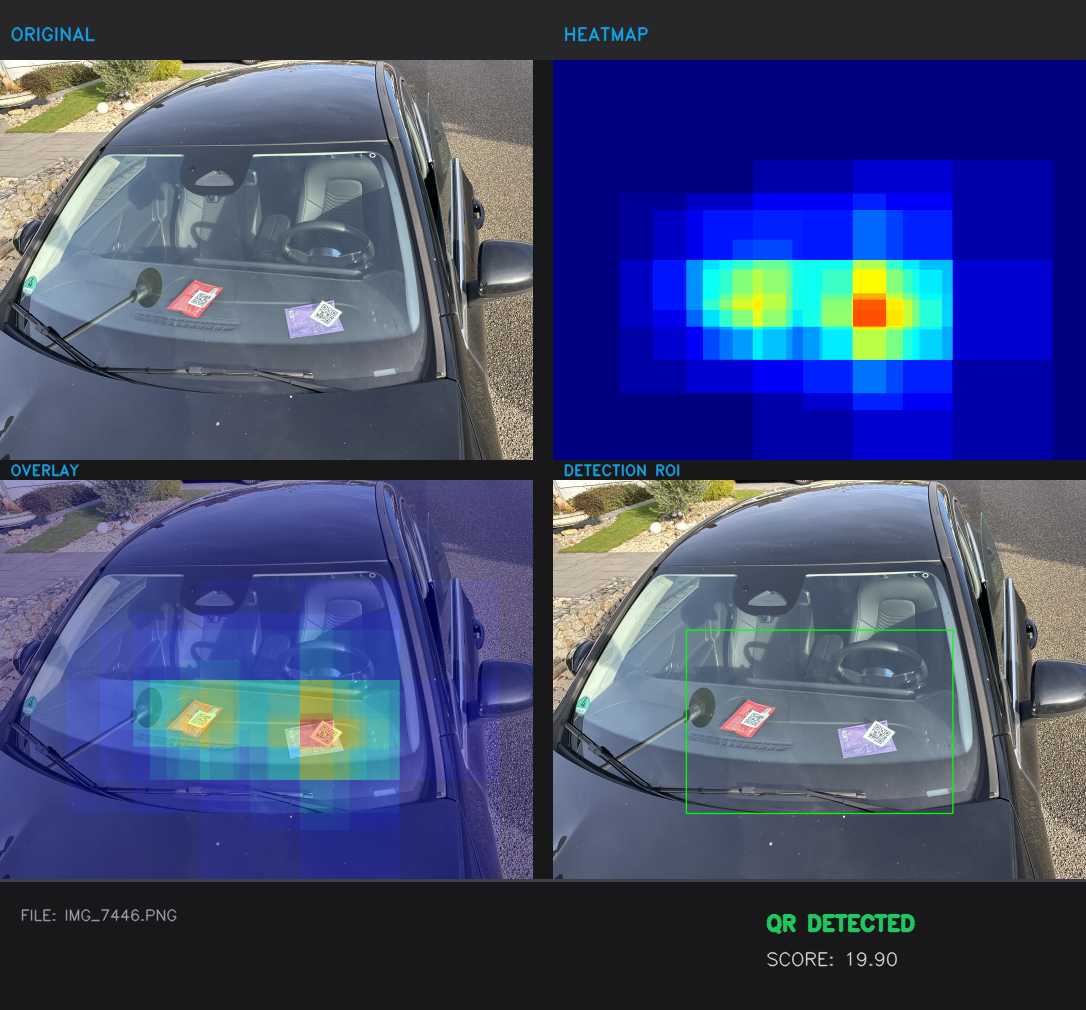
\includegraphics[width=0.8\textwidth]{GUI.png}
    \caption{Dashboardübersicht QR DETECTED.}
    \label{fig:final_decision_with_qr}
\end{figure}

\begin{figure}[H]
    \centering
    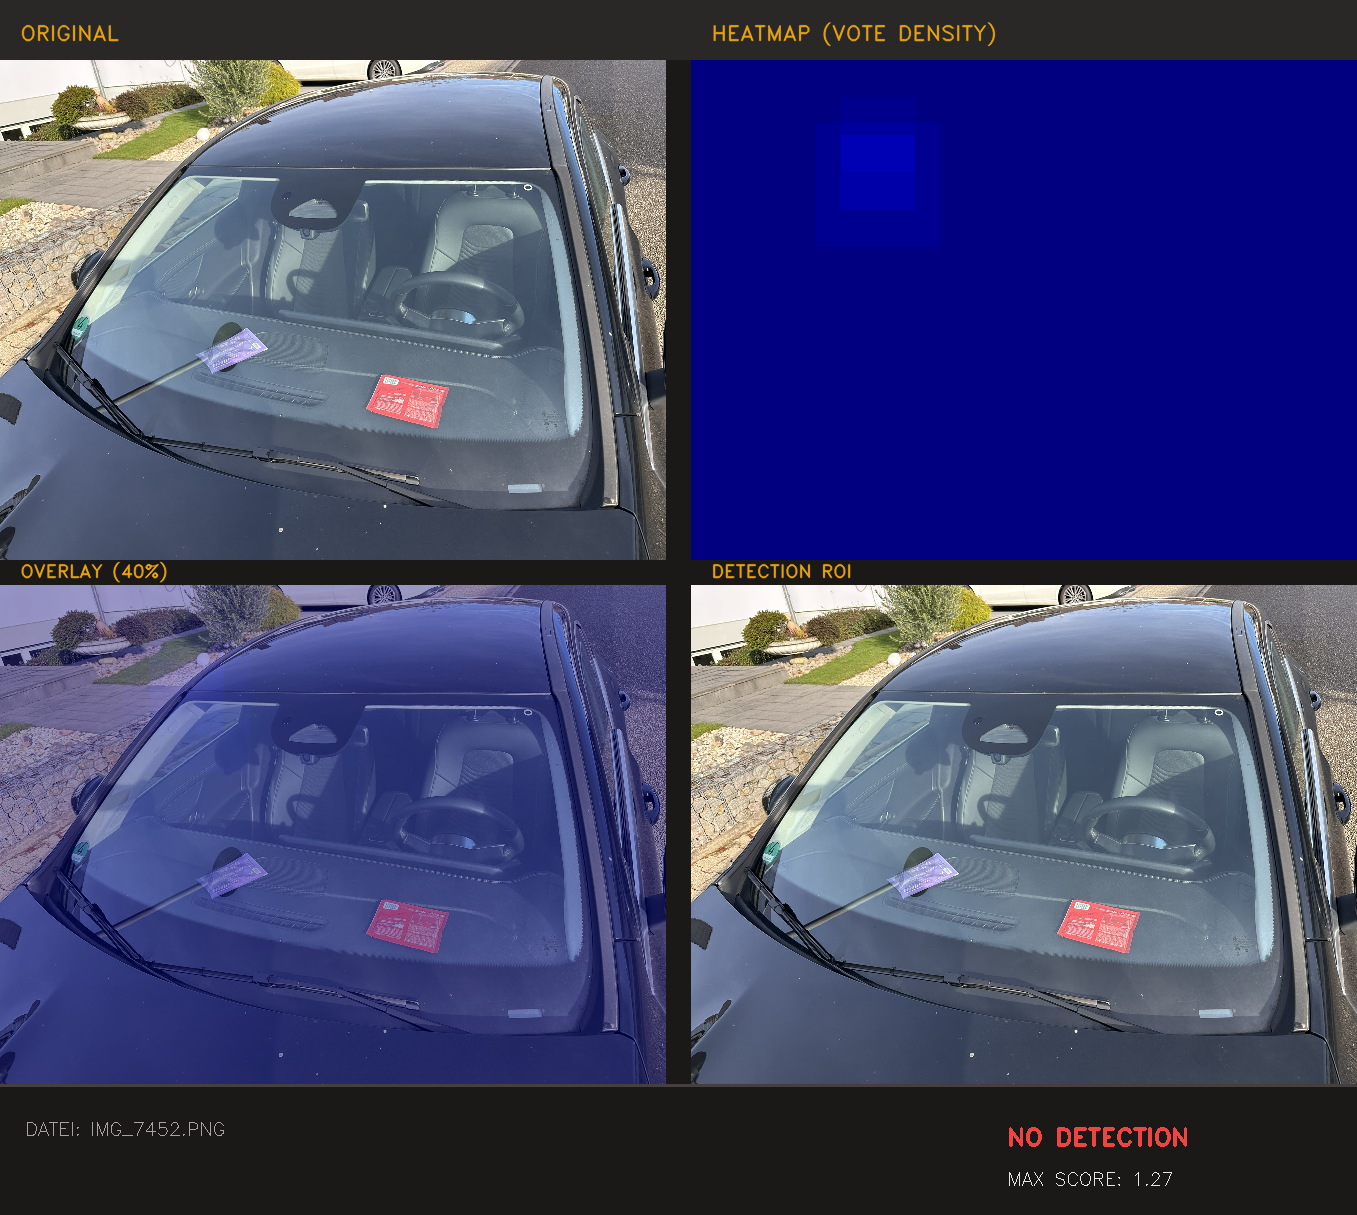
\includegraphics[width=0.8\textwidth]{GUI_negativ.png}
    \caption{Dashboardübersicht NO DETECTION.}
    \label{fig:final_decision_without_qr}
\end{figure}

% ==========================================
% KAPITEL 6: ENTSCHLÜSSELUNG DER QR-CODES
% ==========================================
\section{Entschlüsselung der QR-Codes}

Nachdem die Inferenzphase potenzielle Regionen (ROIs) identifiziert hat, folgt der entscheidende Schritt der Inhaltsanalyse. Ziel ist es, die grafischen Bit-Muster in einen digitalen Datenstring zu überführen. Da die Bildaufnahme unter realen Bedingungen einer Waschanlage erfolgt, muss das System eine hohe Resilienz gegenüber physikalischen Störeinflüssen aufweisen.

\subsection{Aufgabe und Herausforderungen}
Die Schwierigkeit der Extraktion liegt in der massiven Abweichung von einer idealen Scan-Geometrie. Während kommerzielle Handscanner eine frontale, planparallele Ausrichtung erwarten, agiert dieses System unter erschwerten Bedingungen:
\begin{itemize}
    \item \textbf{Perspektivische Distorsion:} Durch den steilen Aufnahmewinkel der Kamera zur Windschutzscheibe wird das Quadrat des Codes zu einem Trapez verzerrt. Dies verschiebt die Position der Datenbits relativ zu den Synchronisationsmustern.
    \item \textbf{Optische Diffraktion:} Wassertropfen auf der Scheibe wirken wie Mikrolinsen, die lokale Kontraste invertieren oder Kanten verschwimmen lassen.
    \item \textbf{Dynamische Reflexionen:} Lichtbrechungen auf der Glasoberfläche überlagern die Bit-Matrix mit Störsignalen, die für klassische Decoder wie Rauschen wirken.
\end{itemize}


\subsection{Methodik: Detaillierte Analyse der Dekodierungsansätze}
Um eine möglichst robuste Erkennung zu gewährleisten, wurden drei technologisch unterschiedliche Strategien entwickelt und an einem umfangreichen Test-Datensatz von insgesamt 4.128 Bildern evaluiert. Davon enthielten 3.111 Bilder einen relevanten QR-Code unter Realbedingungen (Nässe, Schaum, extreme Winkel). Die Ansätze verfolgen grundlegend verschiedene Philosophien: von der klassischen Bildverbesserung über statistische Aufteilung bis hin zu moderner künstlicher Intelligenz.

\subsubsection{Ansatz 1: Pixel-basierte Bildrestaurierung (Robust Restored)}
Dieser Ansatz folgt dem Prinzip der klassischen digitalen Bildbearbeitung. Die Kernannahme ist, dass ein QR-Code primär deshalb nicht gelesen werden kann, weil das Bild zu unscharf, zu kontrastarm oder durch Umwelteinflüsse wie beispielsweise einen leichten Wasserfilm \glqq verwaschen\grqq\ ist. Man kann sich diesen Ansatz wie eine automatische \glqq digitale Brille\grqq\ vorstellen, die versucht, das Bild für den Standard-Scanner zu optimieren.

Schlägt der erste Leseversuch auf dem Originalbild fehl, wird eine Kette von mathematischen Filtern aktiviert, um die Kanten des QR-Codes für den Computer deutlicher hervorzuheben:
\begin{itemize}
    \item \textbf{Detail-Verstärkung (Guided Filtering):} Hierbei wird das Bild in seine Grundstrukturen und seine feinen Details zerlegt. Die feinen Details – also die Kanten der QR-Code-Module – werden gezielt verstärkt, während großflächiges Rauschen unterdrückt wird.
    \item \textbf{Kanten-Schärfung (Laplace-Operator):} Ein mathematischer Filter sucht nach abrupten Helligkeitsübergängen (Schwarz-Weiß-Wechsel) und steilt diese extrem nach. Dies soll verhindern, dass der Scanner die einzelnen Punkte des Codes als grauen Brei wahrnimmt.
\end{itemize}

\begin{lstlisting}[language=Python, caption={Iterative Bildverbesserungskette in Ansatz 1}]
def run_decoding_restored(roi):
    # 1. Versuch: Dekodierung des Rohbildes
    result = decode(roi)
    if result: return result
    
    # 2. Versuch: Kantenanhebung (Detail Enhancement)
    # Ziel: Strukturen klarer vom Hintergrund abheben
    enhanced = cv2.detailEnhance(roi, sigma_s=10, sigma_r=0.15)
    result = decode(enhanced)
    if result: return result
    
    # 3. Versuch: Schaerfungs-Kernel zur Kontrastmaximierung
    kernel = np.array([[-1,-1,-1], [-1,9,-1], [-1,-1,-1]])
    sharpened = cv2.filter2D(roi, -1, kernel)
    return decode(sharpened)
\end{lstlisting}

\textbf{Evaluation:} Trotz der optischen Aufwertung erzielte dieser Ansatz lediglich eine Erfolgsquote von 22,3\,\%. Das Hauptproblem bleibt die Geometrie: Da die Filter zwar die Pixel deutlicher machen, aber die perspektivische Verzerrung (das Trapez) nicht korrigieren, erwartet der Standard-Scanner die Datenpunkte immer noch an der falschen Stelle.

\subsubsection{Ansatz 2: Räumliche Redundanz (Smart Tiling)}
Dieser Ansatz nutzt eine Eigenschaft von QR-Codes aus: ihre eingebaute Fehlertoleranz. Ein QR-Code muss nicht zu 100\,\% perfekt sichtbar sein, um gelesen zu werden; oft reichen schon 70\,\% der Fläche aus, um den Rest mathematisch zu ergänzen.

Die Idee von Divide-and-Conquer\grqq-Verfahren (Teile und Herrsche). Anstatt das gesamte, eventuell teilweise durch Schaum oder Reflexionen gestörte Bild zu scannen, wird die Region in fünf kleinere, überlappende Sektoren zerlegt: das Zentrum sowie die vier Ecken.
Die Logik dahinter: Wenn beispielsweise in der oberen linken Ecke ein dicker Wassertropfen das Bild verzerrt, ist das Zentrum oder die untere rechte Ecke vielleicht noch klar genug. Durch das separate Scannen dieser Teilbereiche erhöht man die statistische Chance, dass der Scanner in einem der Ausschnitte genügend saubere Daten findet, um den gesamten Inhalt zu rekonstruieren.

\begin{lstlisting}[language=Python, caption={Sektorale Aufteilung der ROI (Smart Tiling)}]
def combined_force_decode(roi):
    h, w = roi.shape[:2]
    # Aufteilung in 5 strategische Bereiche
    sectors = {
        "Center": roi[int(h*0.2):int(h*0.8), int(w*0.2):int(w*0.8)],
        "Top-Left": roi[0:int(h*0.7), 0:int(w*0.7)],
        "Top-Right": roi[0:int(h*0.7), int(w*0.3):w],
        "Bottom-Left": roi[int(h*0.3):h, 0:int(w*0.7)],
        "Bottom-Right": roi[int(h*0.3):h, int(w*0.3):w]
    }
    for name, patch in sectors.items():
        if res := robust_decode_func(patch):
            return res, name 
    return None, None
\end{lstlisting}

\textbf{Evaluation:} In der Praxis erwies sich dieser Ansatz als enttäuschend. Die Laufzeit vervielfachte sich, da pro Bild bis zu sechs Dekodierversuche unternommen wurden. Da die grundlegende perspektivische Verzerrung auch in den kleinen Ausschnitten bestehen bleibt, lag die Erfolgsquote kaum über der von Ansatz 1. 

\subsubsection{Ansatz 3: KI-basierte Detektion und Rektifizierung (QReader)}
Der dritte Ansatz unterscheidet sich fundamental von den vorherigen, da er das Problem nicht durch Bildfilter, sondern durch geometrisches Verständnis löst. Hierbei kommt die spezialisierte KI-Bibliothek \texttt{QReader} zum Einsatz.

Dieser Prozess läuft in zwei hochintelligenten Phasen ab:
\begin{enumerate}
    \item \textbf{KI-Suche (YOLOv8):} Ein neuronales Netz, das speziell darauf trainiert wurde, QR-Codes auch unter extremen Winkeln und bei schlechter Sicht zu finden, scannt den Bildbereich. Dabei ist die Empfindlichkeit sehr hoch eingestellt, sodass auch stark verzerrte Codes erkannt werden.
    \item \textbf{Digitale Rektifizierung (\glqq Bügeln\grqq):} Das ist der entscheidende Schritt. Die KI erkennt die vier exakten Eckpunkte des QR-Codes, egal wie schief er im Bild liegt. Mithilfe einer mathematischen Transformation wird der verzerrte Code \glqq geradegezogen\grqq. Er wird virtuell so umgerechnet, als ob die Kamera frontal und perfekt plan davor stünde. Erst dieser perfekt quadratische Ausschnitt wird an den Scanner übergeben.
\end{enumerate}

\begin{lstlisting}[language=Python, caption={KI-gestuetzte Polygon-Extraktion mittels QReader}]
from qreader import QReader
reader = QReader(model_size='s') # Nutzt ein kompaktes YOLOv8-Modell

# Schritt 1: Finden der 4 Eckpunkte (Polygon)
detections = reader.detect(image=roi_rgb) 

for det in detections:
    # Schritt 2: Mathematische Entzerrung und Auslesen
    content = reader.decode(image=roi_rgb, detection_result=det)
    if content:
        # Die Eckpunkte werden fuer die Winkelberechnung gespeichert
        poly_points = det['polygon_xy'] 
\end{lstlisting}

\textbf{Evaluation:} Mit einer Erfolgsquote von 33,9\,\% ist dies der mit Abstand leistungsfähigste Ansatz. Er ist der einzige, der die physikalischen Realitäten einer schrägen Windschutzscheibe wirklich kompensieren kann.

\subsection{Finale Entscheidung}
Die abschließende Evaluation führt zu einer eindeutigen Entscheidung für den \textbf{KI-basierten Ansatz mittels QReader}. Mehrere Faktoren gaben hierfür den Ausschlag:

Erstens ist die \textbf{Robustheit} unerreicht. Während klassische Methoden bei 22,3\,\% stagnieren, ermöglicht die KI-gestützte Rektifizierung eine signifikante Steigerung der Erkennungsrate. Dies ist besonders kritisch, da in einer Waschanlage die zuverlässige Identifikation auch unter schwierigsten Sichtbedingungen gewährleistet sein muss.

Zweitens bietet der Ansatz eine überraschende \textbf{Effizienz}. Obwohl der Einsatz eines neuronalen Netzes komplex klingt, ist die Gesamtlaufzeit geringer als bei Ansatz 2. Anstatt blind verschiedene Filter oder Bildbereiche \glqq durchzuprobieren\grqq, erkennt die KI die Struktur sofort und führt eine gezielte mathematische Korrektur durch.

Zudem bildet die Methode eine sehr gute Datengrundlage für die Folgeaufgabe. Nur QReader liefert zuverlässig die exakten Bildkoordinaten der vier Eckpunkte des QR-Codes. Wie im folgenden Kapitel erläutert wird, ist diese Information zwingend erforderlich, um die Neigung des QR-Codes zu berechnen und die Kamera hardwareseitig nachzujustieren. Ohne diese präzise geometrische Vorarbeit wäre die gesamte nachgelagerte Winkelberechnung technisch nicht umsetzbar.


\subsection{Verarbeitung multipler QR-Codes und Ergebnissicherung}

In der realen Anwendungssituation einer Waschanlage kann es vorkommen, dass sich mehrere QR-Codes oder code-ähnliche Strukturen im Sichtfeld befinden, etwa durch Parkvignetten oder zusätzliche Hinweisschilder hinter der Windschutzscheibe. Das System nutzt hierbei die in Kapitel 6.2.3 beschriebene KI-Architektur, um eine simultane Erfassung aller relevanten Objekte zu ermöglichen.

\subsubsection{Iterative Abarbeitung und logische Zusammenführung}

Anstatt nach dem ersten Fund abzubrechen, arbeitet der Algorithmus alle in der Heatmap identifizierten Regionen (ROIs) nacheinander ab. Innerhalb jeder ROI ist die QReader-Instanz zudem in der Lage, durch die interne Geometrieerkennung auch mehrere, dicht beieinanderliegende Codes individuell zu separieren. Durch diese iterative Schleife wird sichergestellt, dass keine Information im Bild verloren geht, selbst wenn die Heatmap mehrere „Hotspots“ fusioniert hat.

\subsubsection{Visualisierung und Nutzerfeedback}

Zur unmittelbaren Erfolgskontrolle wird das Originalbild mit grafischen Overlays versehen, die eine differenzierte Fehlerdiagnose ermöglichen:
\begin{itemize}
    \item \textbf{Erfolgreiche Dekodierung (Grün):} Validierte Codes werden mit einem grünen Rahmen markiert. Der extrahierte Textstring wird zur direkten Verifikation unmittelbar über der Bounding Box eingeblendet.
    \item \textbf{Nicht lesbare Detektion (Rot):} Erkennt die KI eine eindeutige QR-Geometrie, kann diese aber (z.\,B. durch Schaumbedeckung) nicht dekodieren, wird der Bereich rot umrahmt.
\end{itemize}


\begin{figure}[H]
    \centering
    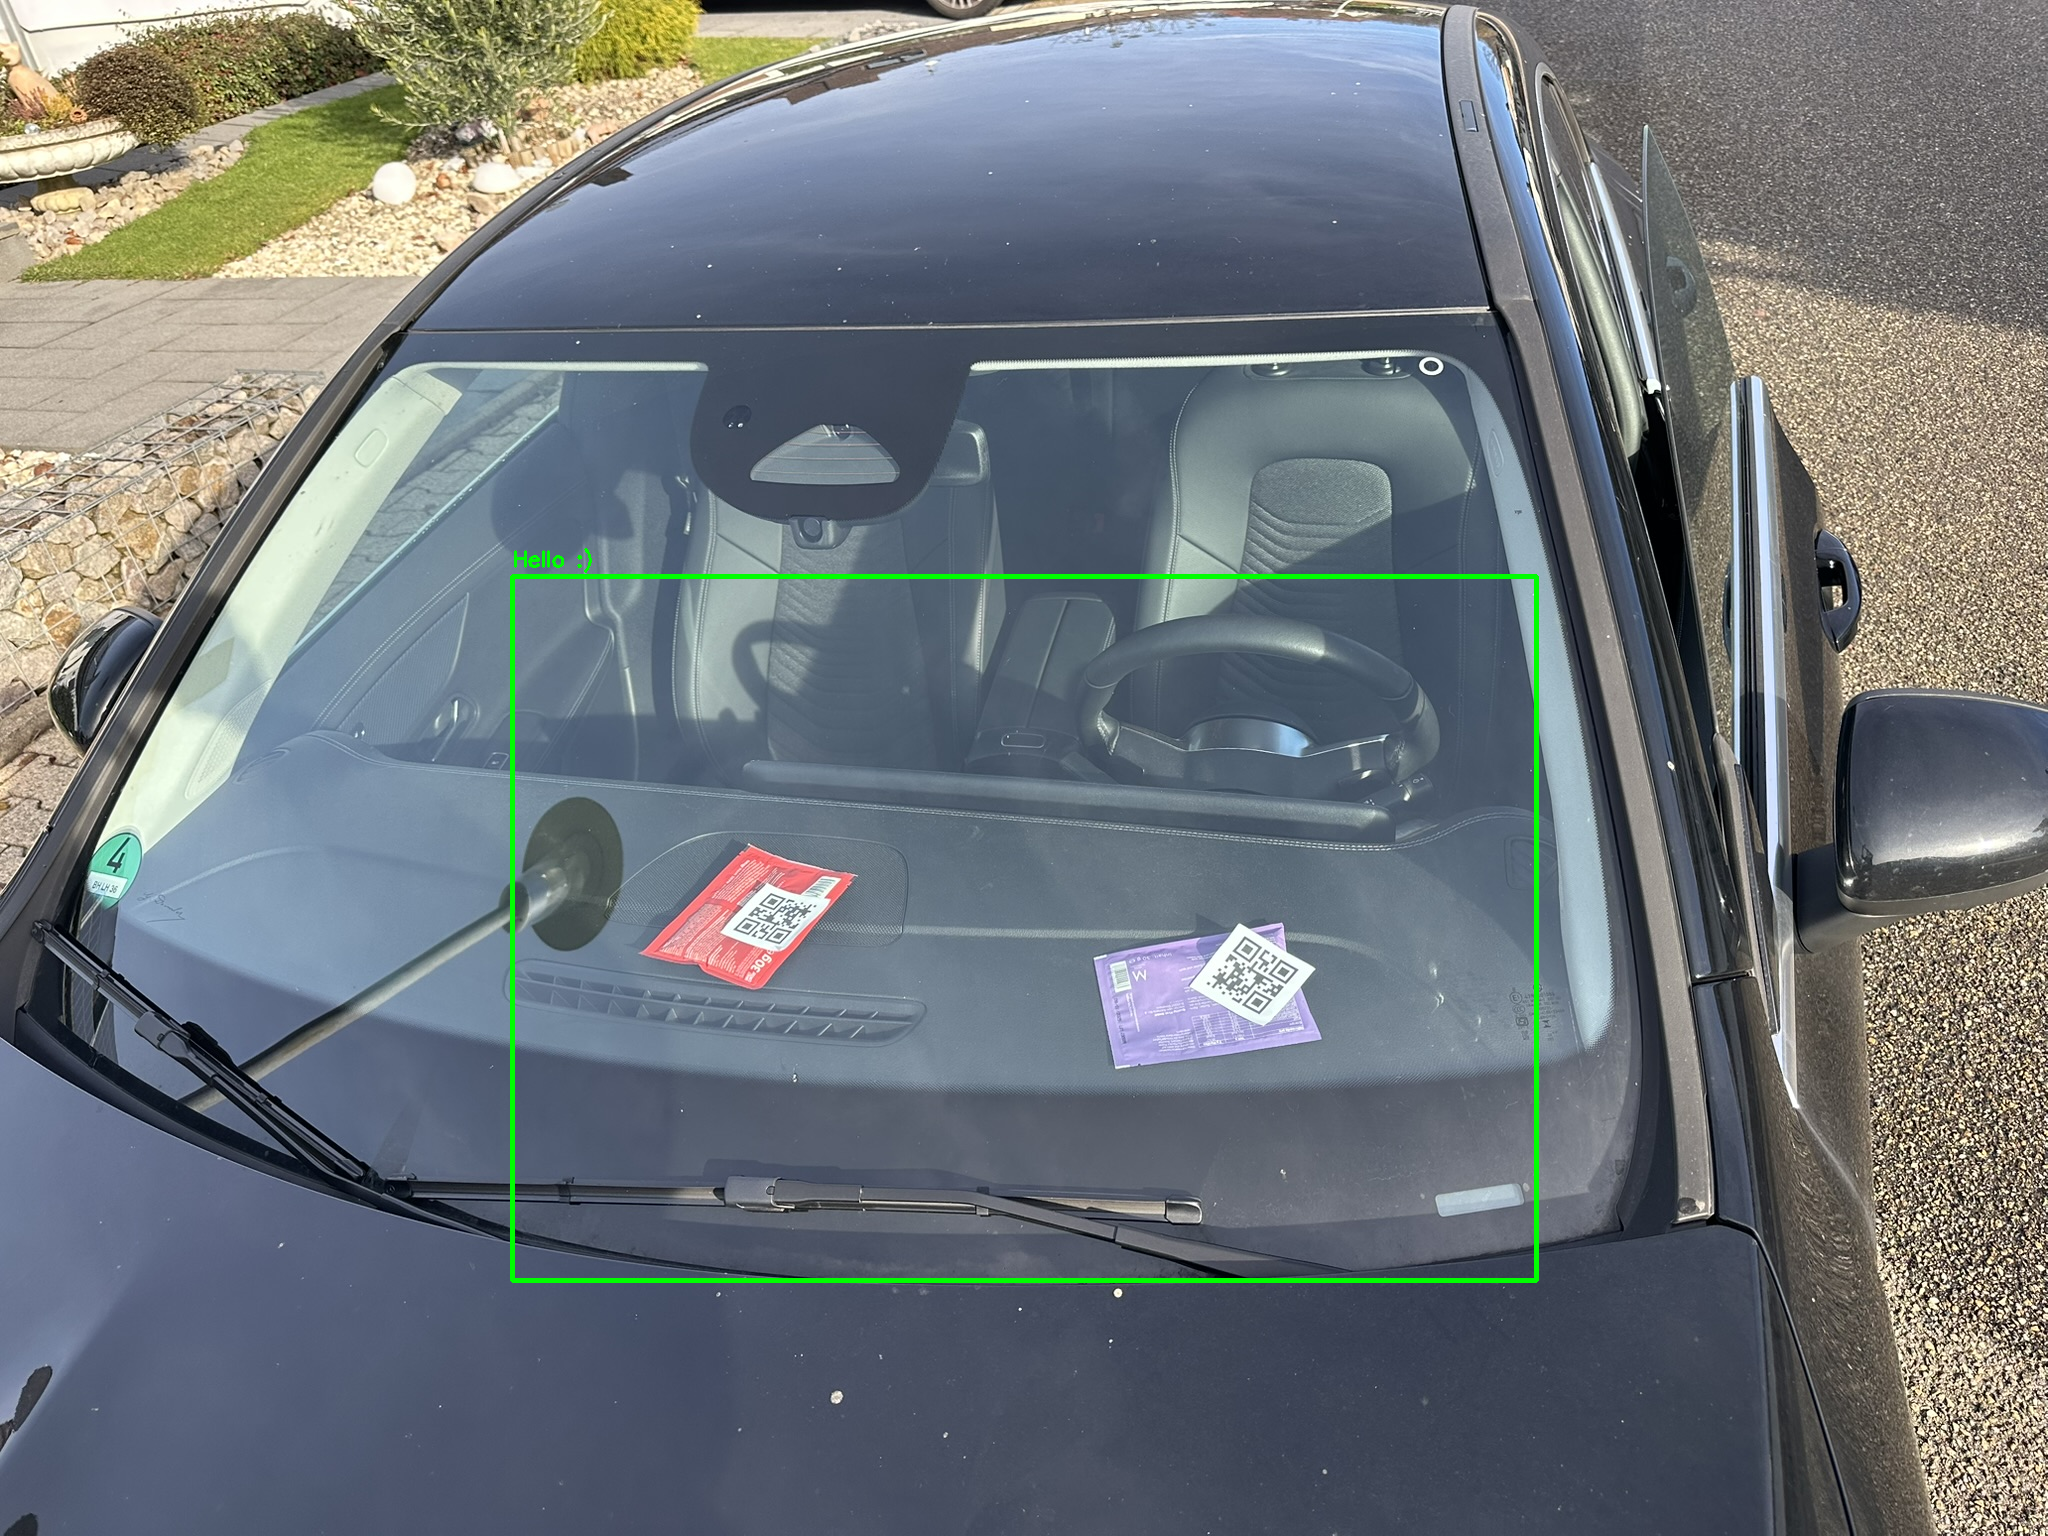
\includegraphics[width=0.8\textwidth]{Entcoded.PNG}
    \caption{Darstellung des entschlüsselten QR-Codes}
    \label{fig:final_decision}
\end{figure}

\subsubsection{Datensicherung und Log-File-Struktur}

Die Ergebnisse werden für die statistische Auswertung in einer semikolon-separierten Textdatei (\texttt{scan\_results.txt}) protokolliert. Dieses Format erlaubt sowohl eine einfache maschinelle Weiterverarbeitung (z.\,B. in Excel oder Python Pandas) als auch eine schnelle manuelle Kontrolle. Die Struktur folgt dem Schema:

\begin{center}
    \texttt{Dateiname;Status;Inhalt}
\end{center}

Ein konkreter Protokolleintrag für eine erfolgreiche Detektion stellt sich wie folgt dar:

\begin{lstlisting}[caption={Beispielhafter Eintrag in der Log-Datei}, frame=single]
IMG_7446.PNG;OK;Hello :)
\end{lstlisting}

Ein Bild wird logisch als \textbf{Erfolg (success)} eingestuft, sofern mindestens ein Code gelesen werden konnte. In diesem Fall wird für jeden gefundenen Inhalt eine eigene Zeile im Log generiert. Nur bei vollständiger Unlesbarkeit aller detektierten Bereiche erfolgt eine Einordnung als \textbf{failed}. Diese Struktur erlaubt eine präzise spätere Analyse der Erkennungsraten unter variierenden Umweltbedingungen, da der Status \texttt{OK} direkt mit dem extrahierten Datenstring korreliert.


% ==============================================================================
% KAPITEL 7: GEOMETRISCHE ANALYSE UND WINKELBERECHNUNG
% ==============================================================================
\section{Geometrische Analyse und Winkelberechnung}

Nach der erfolgreichen Detektion und Dekodierung der QR-Codes besteht die finale Zielsetzung darin, eine präzise Stellgröße für die Schwenkhardware der Kamera zu ermitteln. Dieser Prozess erfordert den Übergang von der zweidimensionalen Bildbetrachtung in eine dreidimensionale räumliche Analyse, um eine optimale Erfassungsgeometrie für den Einsatz in der Waschanlage zu gewährleisten.

\subsection{Methodik: Pose Estimation via SolvePnP}

Zur Bestimmung der räumlichen Orientierung des QR-Codes relativ zur Kamera wird das \textit{Perspective-n-Point} (PnP) Verfahren eingesetzt. Da ein QR-Code eine bekannte, quadratische Geometrie aufweist, lässt sich die perspektivische Verzerrung innerhalb des zweidimensionalen Abbilds mathematisch nutzen, um auf die Neigung der Oberfläche im Raum zurückzuschließen.

Das Verfahren basiert auf dem Abgleich zweier Koordinatensysteme:
\begin{itemize}
    \item \textbf{3D-Modellraum (Weltkoordinaten):} Definition des QR-Codes als ideales, flaches Quadrat im virtuellen Raum (z.\,B. Koordinaten von -5,0 bis +5,0 Einheiten).
    \item \textbf{2D-Bildraum (Pixelkoordinaten):} Die durch die KI detektierten vier Eckpunkte des verzerrten Polygons innerhalb des Kamerabildes.
\end{itemize}

Mittels der mathematischen Funktion \texttt{cv2.solvePnP} wird die Rotation und Translation berechnet, aus welcher der \textbf{Pitch-Winkel} (Neigung um die X-Achse) extrahiert wird. Dieser Winkel repräsentiert die Abweichung zwischen der aktuellen optischen Achse der Kamera und der Normalen (der Senkrechten) der QR-Code-Ebene.

\subsection{Differenzierung der Winkel-Kategorien}

Für die korrekte Interpretation der Ergebnisse ist eine strikte Unterscheidung zwischen zwei Winkeldefinitionen essenziell:

\subsubsection{Der relative Tilt-Winkel (Bildspezifische Messung)}
Dieser Wert wird für jedes analysierte Bild individuell berechnet. Er beschreibt die verbleibende Abweichung zur idealen Draufsicht in einer spezifischen Aufnahme. Ein Messwert von \SI{0}{\degree} würde bedeuten, dass die Kamera bereits perfekt orthogonal (im $90^\circ$-Winkel) zum Code steht. Geringe Werte in den Testreihen, wie beispielsweise \SI{2,2}{\degree}, belegen, dass die Kamera zum Zeitpunkt der Aufnahme bereits nahezu ideal zum Zielobjekt ausgerichtet war.

\begin{figure}[H]
    \centering
    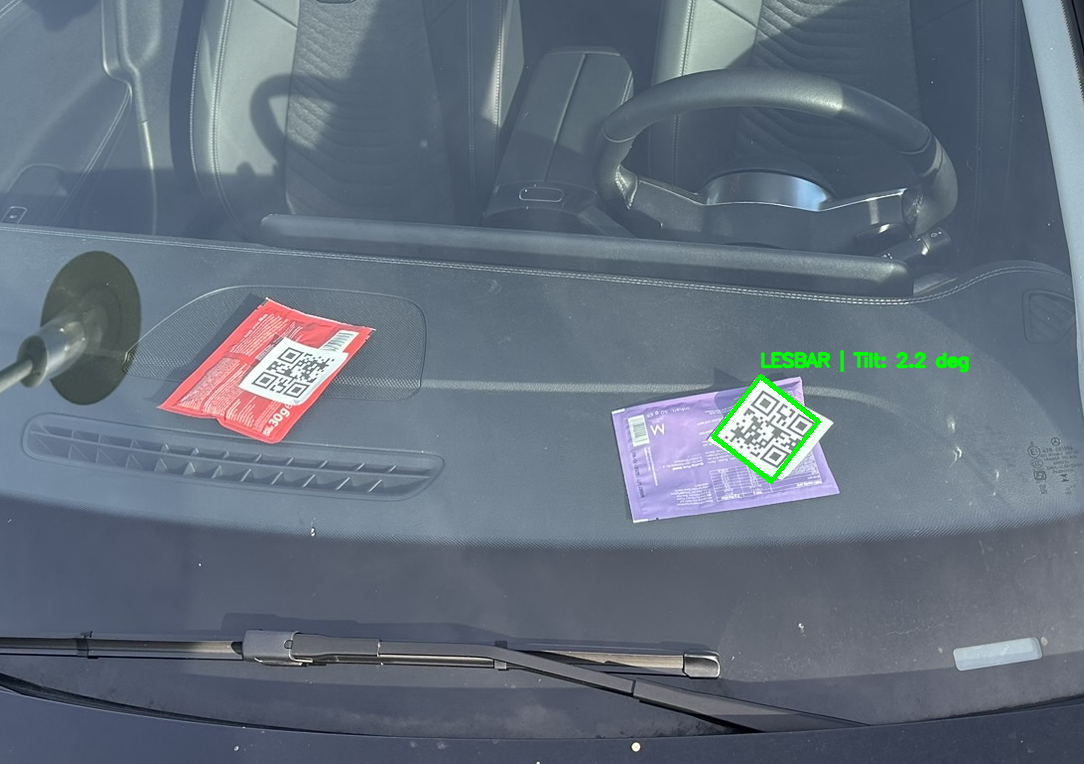
\includegraphics[width=0.8\textwidth]{tilt_winkel.PNG}
    \caption{Einzelbild-Analyse mit Angabe der relativen Winkelabweichung bei lesbarem QR-Code.}
    \label{fig:einzel_tilt}
\end{figure}

\begin{figure}[H]
    \centering
    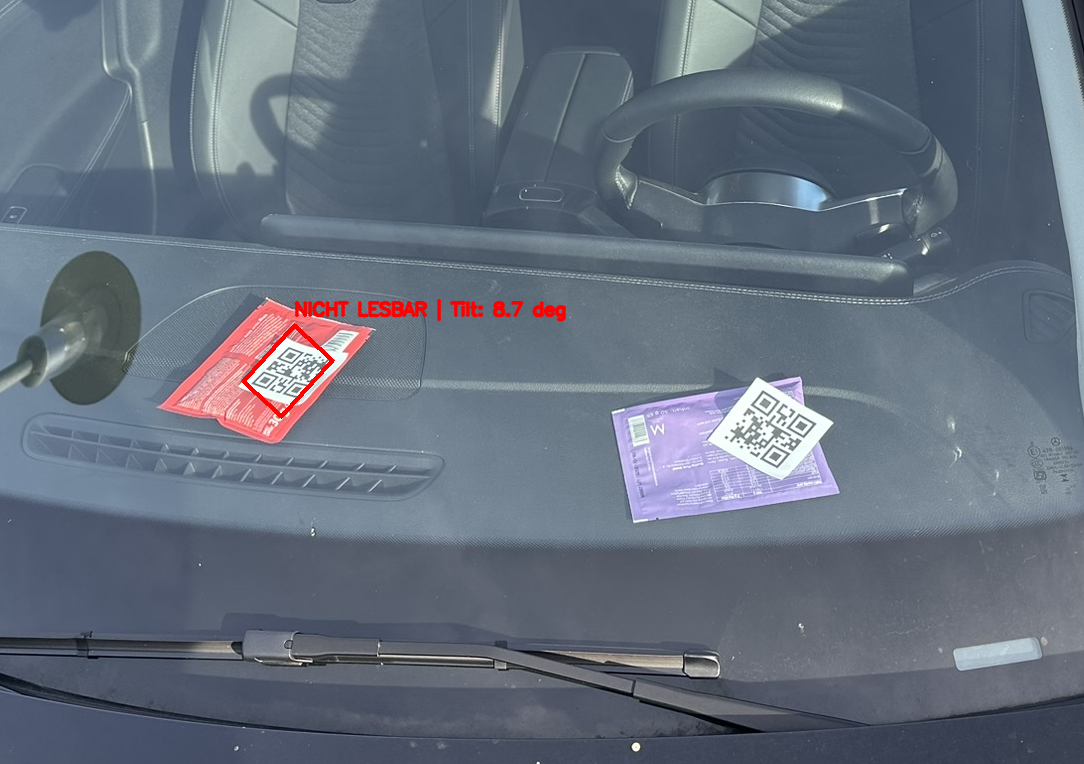
\includegraphics[width=0.8\textwidth]{tilt_winkel_negativ.PNG}
    \caption{Einzelbild-Analyse mit Angabe der relativen Winkelabweichung bei nicht lesbarem QR-Code.}
    \label{fig:einzel_tilt_negativ}
\end{figure}

\newpage

\subsubsection{Der absolute Montage-Winkel (Systemweite Empfehlung)}
Dieser Winkel bezieht sich auf die hardwareseitige Installation der Anlage. Ausgehend von einer horizontalen Grundstellung (Kamera blickt parallel zur Decke) definiert dieser Wert den notwendigen Schwenk nach unten, um den statistischen Durchschnitt der Fahrzeuggeometrien optimal abzudecken.

\subsection{Statistische Auswertung und Ergebnisse}

Um eine belastbare Montageempfehlung auszusprechen, wurde eine Großzahlanalyse über insgesamt 1075 erfolgreich dekodierte Datensätze durchgeführt. Die statistischen Kennzahlen dieser Untersuchung sind in der folgenden Tabelle zusammengefasst:

\begin{table}[H]
    \centering
    \caption{Statistische Kennzahlen der Winkelanalyse (Datengrundlage $n=1075$)}
    \label{tab:winkel_stats}
    \begin{tabular}{l l}
        \toprule
        \textbf{Parameter} & \textbf{Wert} \\
        \midrule
        Minimaler gemessener Winkel & \SI{0,0}{\degree} \\
        Maximaler gemessener Winkel & \SI{68,2}{\degree} \\
        Arithmetisches Mittel (Mean) & \SI{39,5}{\degree} \\
        \textbf{Median (Empfohlener Montage-Winkel)} & \textbf{\SI{44,3}{\degree}} \\
        \bottomrule
    \end{tabular}
\end{table}
Die Entscheidung für den Median als primäre Kenngröße für die Montageempfehlung gegenüber dem arithmetischen Mittel (Mean) begründet sich durch dessen statistische Robustheit. Während das arithmetische Mittel empfindlich auf Extremwerte reagiert – etwa bei vereinzelten Messungen von außergewöhnlich flachen Sportwagen oder sehr hohen Nutzfahrzeugen, bleibt der Median von solchen Ausreißern unbeeinflusst. 

Da die Datengrundlage eine hohe Varianz an Fahrzeugtypen abdeckt, deutet die Differenz zwischen dem Mittelwert (\SI{39,5}{\degree}) und dem Median (\SI{44,3}{\degree}) auf eine asymmetrische Verteilung der Messdaten hin. Der Median repräsentiert in diesem Kontext den Wert, der die Verteilung exakt halbiert, und liefert somit eine stabilere Stellgröße für die mechanische Ausrichtung. Durch die Wahl des Medians wird sichergestellt, dass die Kamera für die Mehrheit der in der Waschanlage vorkommenden Standard-Fahrzeuge eine nahezu ideale orthogonale Sichtachse einnimmt, ohne durch seltene Randfälle verzerrt zu werden.

\subsection{Wissenschaftliche Begründung der Montageempfehlung}

Die ermittelte Empfehlung von ca. \SI{44}{\degree} erscheint zunächst kontraintuitiv, wenn man eine rein horizontale Lage des QR-Codes auf dem Armaturenbrett unterstellt. Dennoch ist dieser Winkel aus physikalischer und praktischer Sicht einer $90^\circ$-Montage (senkrecht nach unten blickend) vorzuziehen:

\begin{enumerate}
    \item \textbf{Prävention von Totalreflexionen:} Eine senkrechte Sichtachse zur Windschutzscheibe würde bei Glasoberflächen zu starken Spiegelungen. beispielsweise der Deckenbeleuchtung, direkt zurück in das Objektiv führen. Durch den gewählten Schwenkwinkel von \SI{44,3}{\degree} werden Reflexionen nach dem physikalischen Prinzip „Einfallswinkel gleich Ausfallswinkel“ am Sensor vorbeigeleitet, was die Lesbarkeit massiv erhöht.
    \item \textbf{Geometrie der Erfassungsdistanz:} Das System muss Codes aus Entfernungen von bis zu \SI{3}{\meter} vor dem Fahrzeug erfassen. Eine schräge Blickrichtung ist hierfür notwendig, da bei einer $90^\circ$-Montage das Fahrzeugdach die Sicht auf das Armaturenbrett verdecken würde, bevor der QR-Code den Sichtbereich der Kamera erreicht.
    \item \textbf{Fahrzeugergonomie:} QR-Codes folgen meist der Neigung der Windschutzscheibe (typischerweise \SI{30}{\degree} bis \SI{55}{\degree}) oder liegen auf gewölbten Armaturenbrettern. Der Median von \SI{44,3}{\degree} bildet den empirischen „Sweet Spot“, um über eine maximale Varianz an Fahrzeugtypen hinweg eine nahezu orthogonale Projektion zu erzielen.
\end{enumerate}

\begin{figure}[H]
    \centering
    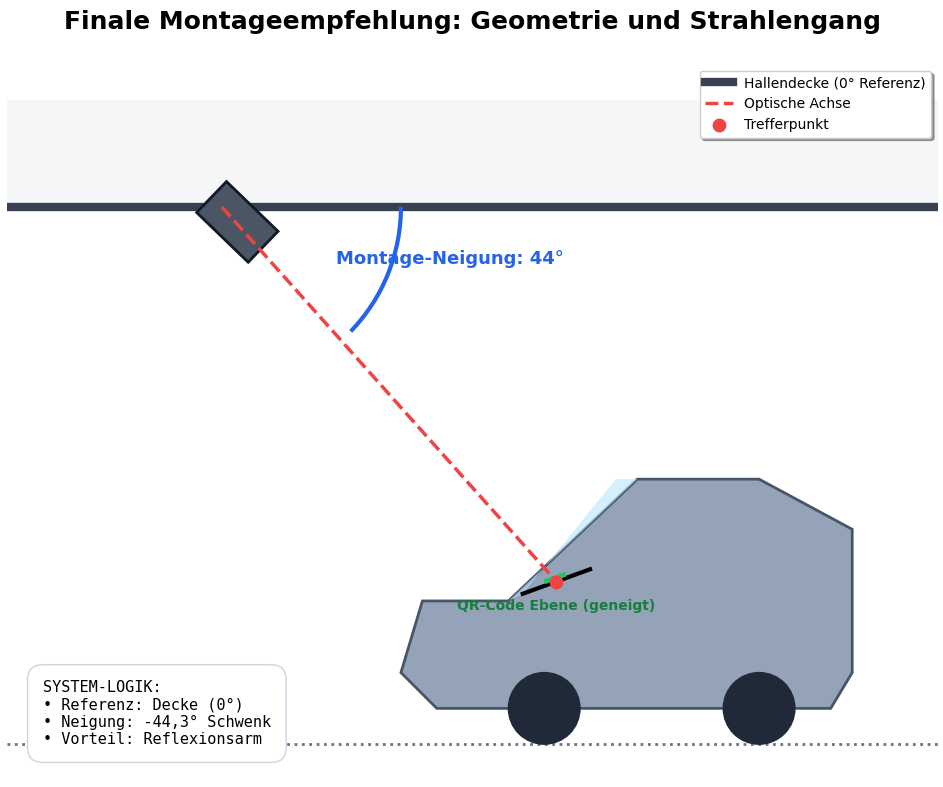
\includegraphics[width=0.8\textwidth]{globale_Winkelempfehlung.png}
    \caption{Schematische Darstellung der Montageempfehlung}
    \label{fig:montage_schema}
\end{figure}
% ==========================================
% ANHANG (Optional)
% ==========================================
%\newpage
%\appendix
%\section{Quellcode}
%\section{Datenblätter}

\end{document}